\documentclass[11pt]{My_preprint}
\usepackage{listing}
%%%%%%%%%%%%%%%%%%%%%%%%%%%%%%%%%%%%%%%%%%%%%%%%%%%%%%%%%%%%%%%%%%%%%%%%%%%%%%%



%%%%%%%%%%%%%%%%%%%%%%%%%%%%%%% Title & Author %%%%%%%%%%%%%%%%%%%%%%%%%%%%%%%%


\title{
    Particle resolved simulation of buoyancy driven motion of monodisperse drops: microstructure modeling with Nearest particle statistics.
    }

\author[1,2]{Nicolas Fintzi}
\author[1]{Jean-Lou Pierson}
\author[2]{Stephane Popinet}
\affil[1]{IFP Energies Nouvelles, Rond-point de l’echangeur de Solaize, 69360 Solaize}
\affil[2]{Sorbonne Universit\'e, Institut Jean le Rond d'Alembert, 4 place Jussieu, 75252 PARIS CEDEX 05, France}
\normalmarginpar


\begin{document}

\maketitle

\begin{abstract}
    In this study, we provide a comprehensive analysis of the various  arrangements that droplets can adopt within dispersed buoyant emulsions. 
    This is termed the study of the microstructure.
    % The study treat both the numerical and theoretical aspects.
    % in a kinetic-theory-like framework.
    To this end, we have developed a novel algorithm capable of effectively prevents numerical coalesce between drops at reasonable computational cost.
    This algorithm is implemented within the Volume of Fluid (VoF) method, utilizing the \href{http://basilisk.fr}{http://basilisk.fr} open source code. 
    Subsequently, we conducted Direct Numerical Simulations (DNS) of statistically steady state mono-disperse buoyant emulsion, over a broad range of \textit{Galileo} number ($Ga$), particle volume fraction ($\phi$), and viscosity ratio ($\lambda$). 
    The density ratio and the \textit{Bond} number are kept constant, $\zeta = 1.11$ and  $Bo = 0.2$, respectively. 
    % In \citet{zhang2023evolution}, it is demonstrated that the microstructure can be characterized effectively using the nearest particle statistic.
    % This approach relies solely on the tensor quantity, \textbf{R}, which represents the second moment of the nearest particle pair distribution.
    % Then, we revisit the \textit{nearest particle statistics} framework of \citet{zhang2023evolution}.
    Then it is shown that, as predicted by \citet{zhang2023evolution}, the second moment of the nearest particle pair distribution, noted \textbf{R}, has the capability to quantify microstructure's features such as clusters and layers of particles.
    In particular, it is found that : 
    (1) At low $Ga$ isotropic clusters appear with increasing $\phi$. 
    (2) Non-isotropic clusters such as layers of particles, are more likely to form for high \textit{Galileo} number.
    (3) The viscosity ratio $\lambda$ has an important impact on the microstructure, clearly more layers are formed for $\lambda = 1$ than $\lambda = 10$. 
    Following this, it is  demonstrated that \textbf{R} follow a kinetic theory-like conservation equation and is governed by a relaxation time $\tau_p$, which is also the average time of interaction between nearest particles pairs. 
    It is shown that $\tau_p$ is higher for $\lambda = 1$ than 
    $\lambda = 10$, and even lower for solid particles at same $Ga$ and $\phi$.
    After, a meticulous analysis of the averaged relative velocity fields between nearest neighbors, we could infer that mechanism such as \textit{Drafting Kissing Tumbling} \citep{fortes1987nonlinear} were present in buoyant emulsions, and that it contribute partly to the formation of the microstructure.
    % Additionally, other behavior are identified in these systems. 
    Overall, our study provides a measure of the microstructure geometry and relaxation time, in terms of $Ga$, $\phi$ and $\lambda$. 
\end{abstract}

\section{Introduction}



\begin{enumerate}
    \item[Intro : ]
    Buoyancy-driven droplet flows are encountered in many chemical engineering processes such as gravity separators, liquid-liquid extractors, etc. The usual engineering practice to model such facilities is to make use of the averaged Navier-Stokes equations and population balance equations. 
    \item[Why is it interesting :]
    However, these methods necessitate closure laws and a deep understanding of particle pair statistics.
    Especially, closures laws are in fact microstructure dependent. 
    Therefore, in an objective to understand to physics these terms it is primordial to understand the microstructure and why it is like so. 
    \item[bibliography : ]
    Previous authors investigated the microstructure of bubbly flows. 
    \citet{bunner2002dynamics} reported the creation of horizontal raft for rising  spherical bubbles. 
    \citet{bunner2003effect} demonstrated taht due to wake trapping effect deformable bubbles have a tendency to align horizontally. 
    In a more recent study \citet{zhang2021direct} also found the creation of horizontal layers of particles. 
    Regarding the solid particles other studies have been conducted for the sedimentation of spheres \citet{shajahan2023inertial}, and they found a high probability of particle pair on  the side of the particle of reference.     
    \item[What is still needed :]
    None, of these studies focus on droplets' suspension. 
    So no closure are available. 
    Additionally, none of them proposed an algorithm to avoid coalesce. 
    \item[What good if i new :]
    An algorithm to prevent coalesce would allow us to perform DNS for arbitrary long time with a fixed population of droplets. 
    In addition to providing data for the closure terms appearing in averaged models, the simulations are of great interest to understand and describe the microstructure of suspensions. 
    \item[introduce the plan :]
    Therefore, within a multiscale strategy, we perform tri-periodic Direct Numerical Simulations (DNS) of monodisperse buoyancy driven suspension of drops.
    In this work we present a concise analysis of the microstructure by analyzing the \textit{Nearest Particle Statistics} recently revisited by \citet{zhang2021ensemble}. 
    We start in \ref{sec:methodo} to present the DNS methodology. 
    Then, we introduce quickly the \textit{nearest particle statistics}.
    In \ref{sec:microstructure} we present an analysis of the microstructure geometry and identify structure such as layers and cluster with respect to the dimensionless parameters. 
    Then, in \ref{sec:time} we describe the relevant timescale of the flow. 

\end{enumerate}

\section{Methodology}
\label{sec:methodo}
In this section we expose the strategy employed to conduct statistically steady state simulations of rising mono-disperse suspension of droplets in a fully periodic domain. 
We start by introducing the physical parameter, followed by a description of the numerical methods.
Lastly, we detail the methodology adopted to collect statistics about microstructure, which are presented in the next sections.

The source code used to perform the DNS is entirely open source.
The simulations are running within the \texttt{Basilisk C} framework, (see \href{http://basilisk.fr}{basilisk.fr}), which is an extension of the C programming language, adapted for the solution of partial differential equations on Cartesian meshes. 
Note that this section is complemented by the wiki page, \href{http://basilisk.fr/sandbox/fintzin/Rising-Suspenion/RS.c}{RS.c}, where the reader can access the source code used to conduct the DNS, as well as comments and notes to help comprehension. 
\tb{la page wiki n'est pas à jour}

This section outlines the approach employed for performing simulations to achieve statistically steady states in the context of a rising mono-disperse suspension of droplets within a fully periodic domain.
We start by presenting the relevant physical parameters, followed by an overview of the numerical methods employed.
Finally, we detail the methodology implemented for collecting statistical data on microstructure, which will be presented in the following sections.

%In this section we expose the strategy employed to conduct statistically steady state simulations of rising mono-disperse suspension of droplets in a fully periodic domain. 
%We start by introducing the physical parameter, followed by a description of the numerical methods.
%Lastly, we detail the methodology adopted to collect statistics about microstructure, which are presented in the next sections.

%The source code used to perform the DNS is entirely open source.
%The simulations are running within the \texttt{Basilisk C} framework, (see \href{http://basilisk.fr}{basilisk.fr}), which is an extension of the C programming language, adapted for the solution of partial differential equations on Cartesian meshes. 
%Note that this section is complemented by the wiki page, \href{http://basilisk.fr/sandbox/fintzin/Rising-Suspension/RS.c}{RS.c}, where the reader can access the source code used to conduct the DNS, as well as comments and notes to help comprehension. 

\subsection{Problem statement}

We investigate numerically the dynamics of homogeneous mono-disperse emulsions subject to buoyancy forces in a fully periodic domain. 
The dispersed and continuous phases are considered Newtonian fluids defined by viscosity $\mu_d$ (resp. $\mu_f$) and density $\rho_d$ (resp. $\mu_f$).
Throughout this work, the subscript $_d$ and $_f$ indicate properties belonging to the dispersed and continuous phases, respectively. 
The interface between both fluids is considered infinitely thin, free of impurities, and characterized by a constant surface tension $\gamma$. %with a coefficient  is assumed. 
The density and viscosity will be considered constant in each phase.
In dimensionless form, this problem is completely characterized by six dimensionless parameters:  the viscosity and density ratio, $\lambda = \mu_d / \mu_f$ and $\zeta = \rho_d / \rho_f$,  
the \textit{Galileo} number, 
\begin{equation*}
    Ga =\frac{\sqrt{\rho_f(\rho_f - \rho_d) g d^3}}{\mu_f},
\end{equation*}
the \textit{Bond} number, 
\begin{equation*}
    Bo =\frac{(\rho_f - \rho_d) g d^2}{\gamma},
\end{equation*}
the number of droplets per domain $N_b$, and the dispersed phase volume fraction $\phi$. 
Here, $d$ represents the diameter of a sphere with the same volume as the droplets and $g$ denotes the acceleration of gravity.
The \textit{Galileo} number measures the strength of the buoyancy forces relative to the viscous forces, whereas the \textit{Bond} number evaluates the ratio between buoyancy and capillary forces. 

%To provide a brief overview of the range of interest for these numbers in an industrial context, let us consider the example of a vegetable oil/water system.
%In most liquid-liquid system encountered in industrial processes the diameter of the droplets lies in the range $d = [50 \mu \text{m}, 3 \text{mm}]$. To provide order of magnitude of the quantities of interest let us consider the example of a vegetable oil dispersed in water. The density and viscosity of the continuous phase are approximately $\rho_f = 1000 \text{kg/m}^3$ and $\mu_f = 10^{-3} \text{Pa.s}$, respectively. The density and viscosity of the dispersed phase are close to $\rho_d = 900 \text{kg/m}^3$ and $\mu_d = 10^{-2} \text{Pa.s}$, respectively.
%We consider the gravitational acceleration on earth, thus $g= 9.81 \text{m.s}^{-2}$.
In most liquid-liquid systems encountered in industrial processes, the droplet diameters typically range from 10 micrometers to a few millimeters. To illustrate the order of magnitude of the relevant quantities, consider a scenario where vegetable oil is dispersed in water. The continuous phase (water) has a density of approximately $\rho_f = 1000 \text{kg/m}^3$ and a viscosity of about $\mu_f = 10^{-3} \text{Pa.s}$. In contrast, the dispersed phase (vegetable oil) has a density close to $\rho_d = 900 \text{kg/m}^3$ and a viscosity around $\mu_d = 10^{-2} \text{Pa.s}$.
The surface tension of the oil/water system is approximately $\gamma = 0.05 \text{N.m}^{-1}$. The maximum allowable volume fraction is set at $\phi = 0.2$. Beyond this value, particles tend to coalesce easily, leading to a loss of the dispersed flow topology.%The maximum volume fraction is set to $\phi = 0.2$, indeed above such $\phi$ particles coalesce easily and the topology of the flow cannot be considered as dispersed anymore. %\citep{de2015gouttes}. 
\begin{table}[h!]
    \centering
    \caption{Dimensionless parameters of a water/oil system.}
    \begin{tabular}{|c||c|c|c|c|c|}
        \hline&$Ga$&$Bo$&$\phi$&$\lambda$&$\zeta$\\ \hline
        \hline Oil/Water&$[0.35,160]$&$[10^{-5};10^{-1}]$&$<0.2$&$10$&$0.9$\\ \hline
    \end{tabular}
    \label{tab:parameters_exp}
\end{table}
\ref{tab:parameters_exp} gives the corresponding dimensionless parameters.  
Notice that the \textit{Bond number} is relatively low, indicating that the droplets are nearly spherical in these processes.
Following \ref{tab:parameters_exp}, to approach real-life applications, we conducted DNS for four volume fractions, specifically $\phi = 0.01,0.05,0.1,0.2$.
In contrast to most previous studies, we keep the number of droplets constant while changing the volume fraction $\phi$. 
We then modify the domain size $\mathcal{L}$ accordingly. 
This introduces another dimensionless parameter of interest: $\mathcal{L}/d$, which measures the confinement of the particles within the finite numerical domain. 
This parameter is purely determined by $\phi$ and $N_b$, and will thus be refereed as a \textit{secondary parameter}.

As mentioned, the \textit{Bond} numbers of our targeted application is very low.
Therefore, the \textit{Bond} number is set to $Bo = 0.2$, and it will stay constant throughout this study.
DNS with lower \textit{Bond} numbers become excessively expensive due to the restrictive capillary time step constraint. 
However, we assert that for $Bo \leq 0.2$, the droplet shape essentially remains spherical, at least for small \textit{Galileo} numbers. 
Additionally, the ratio between inertia and surface tension forces is given by the \textit{Weber} number, 
\begin{equation*}
    We = \frac{\rho U^2d}{\gamma}%\frac{Bo \cdot Re^2}{Ga},
\end{equation*}
%where $Re = \frac{\rho_f d U}{\mu_f}$ is the Reynolds number based on 
where $U$ is the relative velocity which is the difference between the dispersed phase velocity and the continuous velocity.%drift velocity $U$ which is the difference between the dispersed phase velocity and the bulk velocity.
%Values of \textit{Reynolds} numbers for each DNS are provided in \ref{ap:slip_vel} (\ref{fig:Reall}). 
Extreme values of $We$ reached in these simulations are displayed in \ref{tab:simulations}. 
It is clear that for $We=0.6$, we might expect some deformations; nevertheless, in most cases, $We$ stays below these values. 
Consequently, whether in the viscous or inertial regimes, the droplets are expected to remain spherical according to the values of $Bo$ and $We$.
This statement is verified in appendix \ref{ap:deformation}.%will be verified in \ref{sec:microstructure}. 

%Density and viscosity ratio of droplets in real life applications are reported in \citet[Figure 1.]{balla2020effect}.
%As depicted in \citet[Figure 1.]{balla2020effect}, the viscosity and density ratio of fluid-fluid systems range between, $\lambda \in [10^{-4} : 10^4]$ and $\zeta \in [10^{-1} : 10^1]$, respectively. 

The study's primary objective is to investigate the microstructure through the nearest particle pair distribution function.
Thus, obtaining a sufficient number of DNS samples is crucial to ensure statistical convergence. 
Also, the physical quantities measured in the simulations must remain independent of the domain size. 
Therefore, we use a number of particles per domain of $N_b = 125$, roughly what \citet{hidman2023assessing} used for their DNS of fully-periodic buoyant rising bubbles.
Moreover, each DNS lasts for a time: $t^*_\text{end} = 1500 \sqrt{d/g}$.
% It is shown in \ref{ap:validation} that these parameters  are sufficient to obtain well converged statistics.  
\begin{table}[h!]
    \centering
    \caption{Dimensionless parameter range investigated in this work.}
    \begin{tabular}{|ccccccc|ccc|}\hline
        \multicolumn{7}{|c|}{Primary parameters}&\multicolumn{3}{|c|}{Secondary parameters}\\\hline\hline
        $Ga$&$Bo$&$\phi$&$\lambda$&$\zeta$&$N_b$&$t^*_\text{end}$&$\mathcal{L}/d$&$Re$&$We$\\ \hline
        $5\rightarrow 100$&$0.2$&$1\% \rightarrow 20\%$&$10$ \& $1$&$0.9$&$125$&$1500$&$6.7\to 18.7$&$10^{-1}\to 170$&$10^{-4}\to 0.6$\\ \hline
    \end{tabular}
    \label{tab:simulations}
\end{table}
This study presents DNS results with dimensionless parameters in ranges outlined in \ref{tab:simulations}.
In summary, we investigated $5$ \textit{Galileo} number $Ga = 5,10,25,50,100$, $4$ different volume fractions $\phi = 0.01,0.05,0.1,0.2$, and two viscosity ratios $\lambda =1,10$ with $Bo = 0.2$ and $\zeta = 0.9$. %In this study we restrict our attention to a single density ratio, $\zeta = 0.9$.
%Regarding the viscosity ratio, we accomplished DNS for 2 different values, namely $\lambda = 1,10$.
%Lastly, to explore the effect of inertia on the microstructure, the \textit{Galileo} number will vary within the range $Ga \in [5,100]$.
This makes a total of $40$ representative simulations of $N_b = 125$ droplets which last for $t= 1500 \sqrt{d/g}$. 
\subsection{Numerical method}

In this problem, the governing equations consist of the one-fluid formulation of the mass and momentum equation, with an additional transport equation for the dispersed phase indicator function. 
We recall their form here, 
\begin{align}
    \pddt \rho+ \div(\rho\textbf{u})
    &= 0,\\
    \label{eq:dt_urho}
    \pddt (\rho \textbf{u})
    + \div (\rho  \textbf{u} \textbf{u} - \bm\sigma)
    &= (\avg{\rho} - \rho)\textbf{g}
    + \textbf{f}_\gamma,\\
    \label{eq:dt_C}
    \pddt C + \textbf{u}\cdot\grad C  
    &= 0,
\end{align}
% \tb{mettre le link navier stokes solver et faire ca pour le reste }
which are the mass, momentum and colors function transport equation, respectively. 
The scalar fields $C$, represents the color function, which range between $0$ and $1$ to indicate the proportion of fluid and dispersed phase, respectively. 
We introduced the fluid velocity vector $\textbf{u}$ and the Newtonian stress tensor $\bm{\sigma} = -p \textbf{I} + \mu (\grad \textbf{u}+ \grad \textbf{u}^\dagger)$ where $p$ is the pressure fields and $^\dagger$ represents the transpose operator.
Note that the material properties, $\rho$ and $\mu$, take the value of the phases in presence, following the arithmetic average : $\rho = (1-C)\rho_f + C \rho_d$ and $\mu = (1-C)\mu_f + C \mu_d$. 
In our case the arithmetic mean turns out to perform better compared to the harmonic mean, which is often used to interpolate the viscosity for bubbly flows \citet{hidman2023assessing,innocenti2020direct}.
More details about this choice is provided in \ref{ap:validation} (\textit{Case 1.}). 
The capillary force is defined as, $\textbf{f}_\gamma =\textbf{n} \gamma \div \textbf{n} $, where \textbf{n} is the normal at the interface.
Following  \citep{bunner2002dynamics}, we incorporated the artificial body force term, $\avg{\rho}\textbf{g}$, on the right-hand side of \ref{eq:dt_urho}, to maintain a zero-averaged velocity throughout the entire numerical domain.  

To solve these equations we first initialized $125$ spherical droplets within a cubic domain with fully periodic boundary condition. 
We used the open source code \url{http///basilisk.fr} to discretize the governing equations in a multigrid solver. 
The Navier-Stokes equations are discretized with a centered scheme.
The two-phase flow solver uses the Volume of Fluid (VoF) method. 
The interfaces between the droplets and the carrier fluid is reconstructed using the Piecewise Linear Inter-face Calculation or PLIC method \citet[Chapter 5.]{tryggvason2011direct}.
Regarding the treatment of the surface tension force term we refer the reader to \citet{popinet2018numerical} for more details. 
The Basilisk solver has been validated extensively, in the framework of bubbly flow. 
Most of the previous studies \citep{hidman2023assessing,innocenti2020direct} recommend a grid definition of $\Delta/d \ge  30$, where $\Delta$ is the grid spacing. 
In \ref{ap:validation} we carried a mesh independence study and demonstrate that a grid spacing of $\Delta = d/30$ is also suitable in our context.
For readers seeking more detailed information about the solvers, we recommend the wiki pages : \href{http://basilisk.fr/src/navier-stokes/centered.h}{centered.h}, \href{http://basilisk.fr/src/tension.h}{tension.h} and \href{http://basilisk.fr/src/poissson.h}{poissson.h} where he can find the source code of the Navier-Stokes, surface tension and multigrid solver used in this work, respectively. 

With the VoF method droplets and bubbles may experience premature coalesce.
For a detailed discussion on this issue, see  \citet[Appendix B]{innocenti2020direct}.
However, in this work, it is imperative to conserve a specific (mono-disperse) population of droplets over time to accumulate sufficient statistics about the microstructure.
To tackle this issue we present in the next section a novel algorithm which prevent coalescence between droplets, while maintaining a reasonable cost. 






\subsection{The \texttt{no-coalescence.h} algorithm}

In previous studies various methods have been used to avoid coalescence. 
One method is to increase artificially the surface tension coefficient at the interface contact points, as demonstrated in the recent study of \citet{hidman2023assessing}.
% This method seems highly efficient, in terms of simplicity and computational expenses. 
However, it remains unclear if the physical behavior of the droplets interactions is well captured due to the introduction of artificial forces. 
Additionally, its applicability for denser emulsions, up to $\phi = 0.2$, remains uncertain. 
\citet{balcazar2015multiple} developed a multiple-marker level-set method to prevent coalescence, while \citet{zhang2021direct} used a multi-VoF method. 
The latter method consists in assigning to each droplet a different color function so  that the interfaces are reconstructed independently when droplets are in close contact.
Since the representations of the interfaces are independent, droplets in contact never coalesce.  
The latter method may be suitable for our objectives, however, it can be quite expensive as it requires solving a transport equation for each tracer, with one tracer assigned per droplet, meaning $125$ tracers in our case. 
\citet{karnakov2022computing} developed a multi-VoF method which requires a fixed number of tracers for an arbitrary number of droplets.
This approach allows multiple non-touching droplets to belong to the same field, which makes it more efficient than the previous study.
Although this approach shares the same basic principle with the one used here, i.e. coloring adjacent droplets with different colors to avoid coalescence, it differs in term of computational methods. 
In the following we present our methodology that as implemented in the \texttt{Basilisk} framework. 

The challenge here is to assign a tracer to every adjacent droplets to prevent numerical coalesce, while minimizing the number of tracers to reduce computational cost. 
This recalls the famous \textit{Four color map theorem} \citep{appel1977solution} which essentially states that : 
\enquote{every map can be color using only four colors, so that two neighboring region are different colors}. 
In our case, this theorem implies that for any 2D configuration only four VoF tracer are necessary to avoid coalescence\footnote{It is worth noting that for a bi-periodic domain, seven colors are required due to the torus-like topology.  }. 
Therefore, leveraging the \textit{Four color map theorem}, one might be able to significantly reduce the number of VoF tracers required.
Note however that the optimal coloring problem is originally a static problem that need to be solved only once. 
In our case, droplets move around over time thus transforming the static problem into a time-dependent problem. 
Furthermore finding the optimal coloring is known to be difficult (the problem is {\em NP-complete}) and solving it at each timestep would be too expensive.

Note also that in three-dimensions the \textit{Four color map theorem} has no equivalent.
For example, an arbitrary large number of rectangular blocks in 3D-space can all touch each other, requiring an arbitrary large number of colors to differentiate the adjacent blocks\citep{magnant2011coloring}. 
We are not aware of an extension of the coloring problem to arrangements of spheres in 3D. 
Nevertheless, it is reasonable to assume that the number of tracers required to avoid coalescence is significantly smaller than the number of droplets.
Consequently, since we cannot determine the optimal coloring configuration based on theoretical grounds, we opt to assign the tracers to each droplet following the empirical strategy detailed below.

The development of the \texttt{no-coalesce.h} algorithm was initiated in the PhD. thesis of \citet{mani2021numerical}.
The latest version of this algorithm can be found on the basilisk wiki page : \href{http://basilisk.fr/sandbox/fintzin/Rising-Suspenion/no-coalescence.h}{no-coalescence.h}.
Before  diving into a step-by-step description of this algorithm we need to introduce another key feature used in these simulations, which is the \href{http://basilisk.fr/src/tag.h}{tag.h} algorithm. 
It is an adaptation of the \textit{painter}'s algorithm, but optimized using the multigrid solver of \texttt{Basilisk}. 
Its purpose is to assign different scalars values to each cell belonging to different regions, with the regions being delimited by the different droplets' interfaces. 
For instance, on \ref{fig:images} (left) we can see two blue regions corresponding to two different drops.
We can notice that both are assigned with two different values, $1$ and $2$, which are identified using the \texttt{tag.h} algorithm. 
It is then straightforward to obtain the droplet properties, such as its center of mass, by carrying numerical integration on the VoF field considering only the cells having a specific tag value, which corresponds to a given droplet.  
% In general, we are able to differentiate droplets' domain, belonging to the same tracer thanks to the \texttt{tag.h} algorithm.


We define the $i^\text{th}$ color function as $C_i$ for $i =1,2,\ldots,N(t)$, where $N(t)$ is the total number of tracers used in a simulation at time $t$.
The color function introduced previously is now defined as, $C = \sum_{i=1}^{N(t)} C_i$. 
Note that $N(t)$ is time-dependent since the number of tracers may increase during the simulation as droplets get closer to one another.
The simplified workflow of the algorithm follows these four steps : 
\begin{enumerate}
    \item[\textit{Step 1}.] Check if within a tracer field $C_i$, the droplets are possibly too close to each other. 
    The \textit{near contact} criterion that determines if the droplets are too close is defined using a $5$ by $5$ cells stencil which verifies the following conditions : 
    (1) If the color function $C_i = 0$ at the center of the stencil. 
    (2) And if $C_i > 1$ for two opposite cells in the stencil. 
    In this case two different regions might be in close contact.
    A sketch of this situation is given in \ref{fig:criterion}.  
    \item[\textit{Step 2}.] 
    If (\textit{Step 1}.) is true for the tracer $C_i$, we must verify if we indeed identified two different regions in near contact, and not just a single region close to itself, such as in \ref{fig:diagram} (right). 
    Therefore at this step  we apply the \texttt{tag.h} algorithm.
    \item[\textit{Step 3}.] Re-use the \textit{near contact} criterion of (\textit{Step 1}.) by requiring in addition that the cells must belong to two different tag groups. 
    At this stage the situation in \ref{fig:criterion} (left) would be true, while the situation on \ref{fig:criterion} (right) would be false. 
    We therefore identified all the droplets / region that are indeed too close to each other. 
    \item[\textit{Step 4}.] 
    Find a new tracer field $C_n$, with which we could set the region/droplets that are in near contact. 
    At this stage, it is essential to identify the list of tracer $C_j$ already in contact with the region to be replaced. 
    For example, in \ref{fig:criterion} (left), the droplet on the right is clearly adjacent to a region with tracer $C_j$, in which case $C_n$ must satisfy $n \neq i,j$. 
    Therefore, any $n$ in $1, 2, \ldots, N(t)$ are suitable candidates as long as this situation is avoided. 
    If the droplet is already adjacent to every tracer $C_j$ in the simulation, for $j = 1, 2, \ldots, N(t)$, we create a new tracer $C_n$ with $n = N(t)+1$ and assign the drop to this tracer field.
\end{enumerate}
\begin{figure}
    \centering
    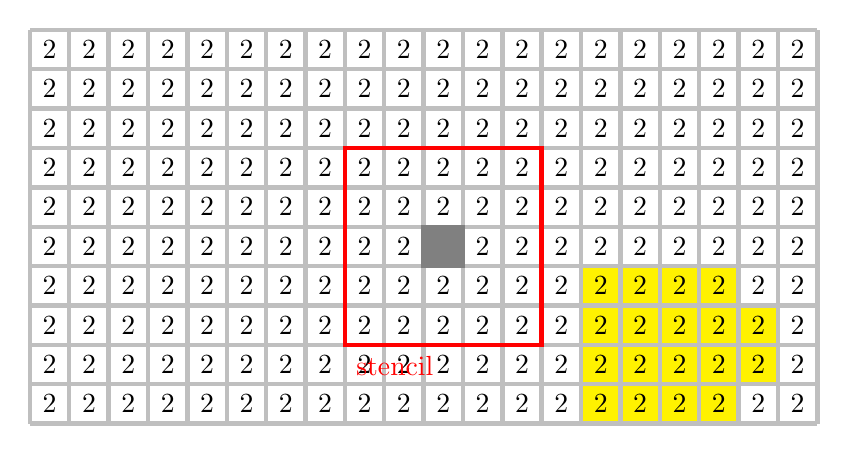
\begin{tikzpicture}[scale=0.5,ultra thick]
        % Define grid dimensions
        \def\nRows{10}
        \def\nCols{20}
        \pgfmathsetmacro\nRowsm{\nRows-1}
        \pgfmathsetmacro\nColsm{\nCols-1}

        \foreach \row in {0,...,\nRowsm} {
            \foreach \col in {0,...,\nColsm} {
                \pgfmathsetmacro\distance{veclen(\col-4.356, \row-2.65)};
                \pgfmathparse{\distance < 4 ? "blue" : "white"}
                \edef\colour{\pgfmathresult};
                \ifthenelse{\equal{\colour}{blue}}{                    
                    \fill[\colour!60!white] (\col, \row) rectangle ++(1,1);
                    \node (num) at (\col +0.5,\row+0.5){1};
                }
            }
        }

        \foreach \row in {0,...,\nRowsm} {
            \foreach \col in {0,...,\nColsm} {
                \pgfmathsetmacro\distance{veclen(\col-15, \row-6.2)};
                \pgfmathparse{\distance < 3.5 ? "blue" :"white"}
                \edef\colour{\pgfmathresult};
                \ifthenelse{\equal{\colour}{blue}}{
                    \fill[\colour!60!white] (\col, \row) rectangle ++(1,1);
                \node (num) at (\col +0.5,\row+0.5){2};
                }
            }
        }

        \foreach \row in {0,...,\nRowsm} {
            \foreach \col in {0,...,\nColsm} {
                \pgfmathsetmacro\distance{veclen(\col-15.62, \row-1.5)};
                \pgfmathparse{\distance < 2.5 ? "yellow" :"white"}
                \edef\colour{\pgfmathresult};
                \ifthenelse{\equal{\colour}{yellow}}{
                    \fill[\colour] (\col, \row) rectangle ++(1,1);
                    \node (num) at (\col +0.5,\row+0.5){2};
                }
            }
        }
        % Define grid size
        \pgfmathsetmacro\gridSize{1}
        
        \foreach \row in {0,...,\nRows} {
            \draw [gray!50] (0,\row*\gridSize) -- (\nCols*\gridSize,\row*\gridSize);
        }
        % Draw vertical grid lines
        \foreach \col in {0,...,\nCols} {
            \draw [gray!50] (\col*\gridSize,0) -- (\col*\gridSize,\nRows*\gridSize);
        }
        % Draw drop shape
        \draw[red] (8,2)node[below right]{stencil} rectangle +(5,5); % Draw the rectangular base
        \filldraw[gray] (10,4) rectangle +(1,1);
    \end{tikzpicture}    
    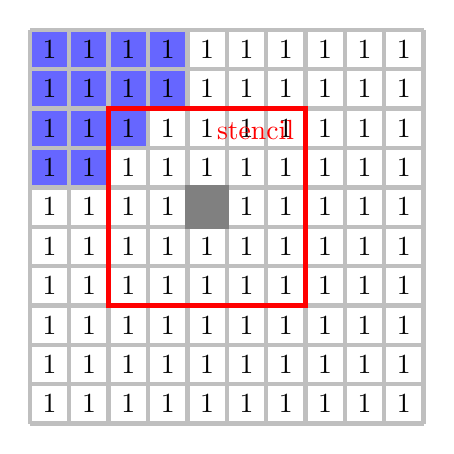
\begin{tikzpicture}[scale=0.5,ultra thick]
        % Define grid dimensions
        \def\nRows{10}
        \def\nCols{10}
        \pgfmathsetmacro\nRowsm{\nRows-1}
        \pgfmathsetmacro\nColsm{\nCols-1}

        \foreach \row in {0,...,\nRowsm} {
            \foreach \col in {0,...,\nColsm} {
                \pgfmathsetmacro\distance{veclen(\col, \row-2)};
                \pgfmathparse{\distance < 3.5 ? "blue" :"white"}
                \edef\colour{\pgfmathresult};
                \ifthenelse{\equal{\colour}{blue}}{
                    \fill[\colour!60!white] (\col, \row) rectangle ++(1,1);
                \node (num) at (\col +0.5,\row+0.5){1};
                }
            }
        }

        \foreach \row in {0,...,\nRowsm} {
            \foreach \col in {0,...,\nColsm} {
                \pgfmathsetmacro\distance{veclen(\col-7, \row-2)};
                \pgfmathparse{\distance < 3.5 ? "blue" :"white"}
                \edef\colour{\pgfmathresult};
                \ifthenelse{\equal{\colour}{blue}}{
                    \fill[\colour!60!white] (\col, \row) rectangle ++(1,1);
                    \node (num) at (\col +0.5,\row+0.5){1};
                }
            }
        }
        \foreach \row in {0,...,\nRowsm} {
            \foreach \col in {0,...,\nColsm} {
                \pgfmathsetmacro\distance{veclen(\col-5, \row)};
                \pgfmathparse{\distance < 3.5 ? "blue" :"white"}
                \edef\colour{\pgfmathresult};
                \ifthenelse{\equal{\colour}{blue}}{
                    \fill[\colour!60!white] (\col, \row) rectangle ++(1,1);
                    \node (num) at (\col +0.5,\row+0.5){1};
                }
            }
        }
        \foreach \row in {0,...,\nRowsm} {
            \foreach \col in {0,...,\nColsm} {
                \pgfmathsetmacro\distance{veclen(\col, \row-9)};
                \pgfmathparse{\distance < 3.5 ? "blue" :"white"}
                \edef\colour{\pgfmathresult};
                \ifthenelse{\equal{\colour}{blue}}{
                    \fill[\colour!60!white] (\col, \row) rectangle ++(1,1);
                    \node (num) at (\col +0.5,\row+0.5){1};
                }
            }
        }
        % Define grid size
        \pgfmathsetmacro\gridSize{1}
        
        \foreach \row in {0,...,\nRows} {
            \draw [gray!50] (0,\row*\gridSize) -- (\nCols*\gridSize,\row*\gridSize);
        }
        % Draw vertical grid lines
        \foreach \col in {0,...,\nCols} {
            \draw [gray!50] (\col*\gridSize,0) -- (\col*\gridSize,\nRows*\gridSize);
        }
        % Draw drop shape
        \draw[red] (2,3) rectangle +(5,5)node[below left]{stencil}; % Draw the rectangular base
        \filldraw[gray] (4,5) rectangle +(1,1);
    \end{tikzpicture}    
    \caption{Sketch of two situations were the \textit{near contact} criterion is true. 
    The background grid represents the cells within the numerical domain. 
    The dark blue area represents the cells where $C_i > 0$.
    The yellow area represents the cells where the tracer $C_j > 0$ for $j\neq i$. 
    The numbers represent the values of the $Tag$ scalar field within each tracer.
    The $5$ by $5$ cells red rectangle represents the stencil zone which iterates over all cells of the domain.  
    %  where the center of the stencil (gray square) must respect $C_i = 0$. 
    (left) Two droplets in contact since we have two opposite cells in the stencil with $C_i > 0$ and $C_i=0$ at the center.
    And the mentioned cells belong to two different regions so that (\textit{Step 3}) is also validated.  
    (right) A near contact is observed since we have two opposite cells in the stencil with $C_i > 0$ and $C_i=0$ at the center, however in this case we do not verify the second criterion of \textit{Step 3} which requires two different tags values. 
    }
    \label{fig:criterion}
\end{figure}
These four steps are executed at each simulation time step and for each tracer $C_i$ with $i = 1, 2, \ldots, N(t)$.
Following this procedure, we ensure that all adjacent droplets are using different tracers, which ultimately prevents coalescence. 

Having $N(t)$ tracers requires some modifications to the aforementioned governing equations. 
Specifically, instead of solving \ref{eq:dt_C}, we solve $N(t)$ transport equations, one for each $C_i$.
Likewise, the surface tension force is computed as the sum of the contributions from each $C_i$ and reads
\begin{align*}
    \pddt C_i + \textbf{u}\cdot\grad C_i = 0,
    \ \  \ \ \forall i = 1,2,\ldots N(t),\\
    \textbf{f}_\gamma 
    = \sum_{i=0}^{N(t)} \gamma \kappa_i \grad C_i
\end{align*}
where $\kappa_i$ is the numerical approximation of the curvature of the interface of field $C_i$, which is computed following the same method employed for a single tracer. 

\ref{fig:diagram} (left) shows a snapshot of a simulation at an arbitrary time $t^* = 100 \sqrt{g/d}$. 
The droplet interfaces are colored by the indices of their respective tracer. 
In this simulation at that time, no more than 3 colors are needed to avoid coalescence.
On \ref{fig:diagram} (right) we display the value of $N(t)$ in term of the dimensionless simulation time for various volume fractions $\phi$ at $Ga = 50$ and  $\lambda = 1$. 
We observe that for the entire simulation, no more than 3 tracers were needed for the dilute emulsion ($\phi = 0.01$) and up to 7 for the denser regime ($\phi = 0.2$). 
Although our algorithm might not be optimized, it brings sufficient efficiency for our needs. 
Indeed, \ref{tab:performance} reports the time spent by each function during a simulation. 
It is observed that the \texttt{no-coalesce.h} algorithm accounts for approximately $4\%$ of the total computational time of a simulation. 
As for the \texttt{tag.h} algorithm, its cost is around $2\%$, which is also reasonable.
In comparison, the \texttt{poisson.h} solver is about $13\%$ of the simulation time. 
The advection of VoF tracers is about $7\%$ which is relatively high but still reasonable.
To reduce the cost related to the \texttt{no-coalesce.h} algorithm we believe that further developments, which are referenced at \href{http://basilisk.fr/sandbox/fintzin/Rising-Suspenion/no-coalescence.h}{no-coalescence.h}, are still doable and could be useful for future studies.
\begin{figure}[h!]
    \centering
    \begin{tikzpicture}
    \node (img) at (0,0) {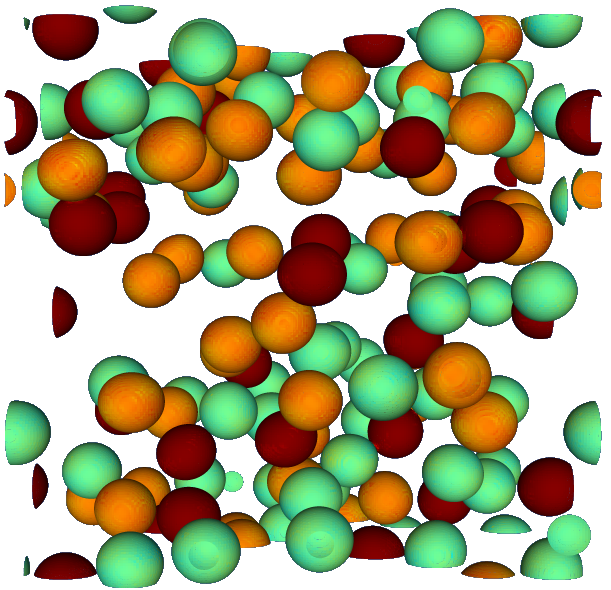
\includegraphics[width = 0.4\textwidth]{image/VoF2.png}};
    \node (img) at (0.4\textwidth,-0.01\textwidth) {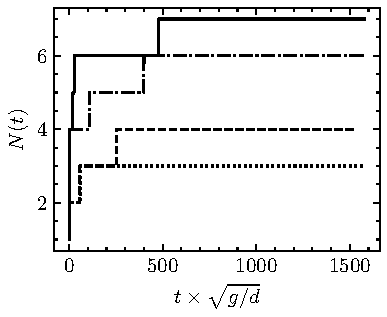
\includegraphics[width = 0.4\textwidth]{image/HOMOGENEOUS_NEW/CA/NVoF_vs_t_Ga_50_l_1.pdf}};
    \end{tikzpicture}
    \caption{
    (left) Snapshot of a DNS with $\phi = 0.05$, $\lambda = 1$, $Ga = 50$ with the interface of the droplets colored by the index of the tracers.
    (right) Number of tracers $N(t)$ as a function the dimensionless time.
    Four different volume fractions are displayed : (dotted line) $\phi = 0.01$, (dashed line) $\phi = 0.05$ (dash dotted line) $\phi = 0.1$ (solid line) $\phi = 0.2$ at $Ga = 50$ and $\lambda = 1$. 
    }
    \label{fig:diagram}
\end{figure}


In order to validate our numerical methodology, we have compared our numerical results to the experiments of \citet{mohamed2003drop} where they experimentally study the impact of a single drop on a flat interface of the same fluid. %, while recording the positions of the interfaces.
It is found that the multi-VoF method captures remarkably well the position of interfaces, even with a poor description of the liquid film between these interfaces.
Additionally, we argue that the mesh independence study conducted in \ref{ap:validation} (Case 3) substantiates the accuracy of the DNS, as the dynamics of interaction do converge with  reasonable errors for a grid resolution of $\Delta/d = 30$. 
Overall, we used an optimized multi-VoF method, enabling us to perform DNS with a maximum of 7 tracers in the densest scenario.
 










\subsection{The nearest particle statistics}


To study the emulsions' microstructure, we chose to adopt the \textit{nearest particle statistics} framework recently revisited by \citet{zhang2021ensemble}.
We now recall some definitions of the \textit{nearest particle statistics} averaging procedure. 
For further details, readers are encouraged to refer to \citet{zhang2023evolution} on which this work mostly relies.

\subsubsection*{Theoretical framework}
Let $P(\FF)$ be the probability density function that describes the probability of finding the flow in the configuration $\FF$, where $\FF = (\lambda_1,\lambda_2,\lambda_3,\ldots)$ is a finite set of all the parameters describing the initial flow configuration.
% \footnote{We assume that the flow can be described by a finite number of parameters related to both phase.}. 
Then, we define $d\mathscr{P} = P(\FF)d\FF$ as the probable number of realizations in the incremental region of the flow' phase space, $d\FF$ around $\FF$.
Additionally,  $\textbf{x}_i(t,\FF)$ and $\textbf{x}_j(\FF,t)$ refers to the Lagrangian position vectors of the particles $i$ and $j$, respectively. 
We also introduce the age of the interaction, denoted as $a$, which represents the time elapsed since two particles became nearest neighbors.
Then, the nearest pair probability density function is given by,
\begin{equation}
    P_{nst}(\textbf{x},\textbf{r},a,t)= 
    \int \sum_{i}^{N_b}\delta(\textbf{x}-\textbf{x}_i)
    \sum_{j\neq i}^{N_b}\delta(\textbf{x}+\textbf{r}-\textbf{x}_j) 
    \delta(t+a-t_c^{ij}) 
    h_{ij} d\mathscr{P},
    \label{eq:P_nstij}
\end{equation}
where we introduced the function $h_{ij}$, which equals $1$ if and only if particle $j$ is one of the nearest neighbors of particle $i$, and $h_{ij} = 0$ otherwise. 
$t_c^{ij}(\FF,t)$ represents the time at which particles $i$ and $j$ became nearest neighbors. 
Formally, we have $a = t - t^{ij}_c(\FF,t)$.
Consequently, $P_{nst}(\textbf{x},\textbf{r},t,a)$ is the probability of having a particle center of mass located at $\textbf{x}$ at time $t$ with it nearest neighbor at $\textbf{x}+\textbf{r}$ given that the pair of particles have been nearest neighbors since $a$ time.
Note that $P_\text{nst}(\textbf{x},\textbf{r},t,a)$ is related to the number density $n_p(\textbf{x},t)$ through the relationship, 
\begin{equation*}
    \int_0^\infty 
    \int_{\mathbb{R}^3}
     P_\text{nst}(\textbf{x},\textbf{r},t,a) d\textbf{r} da = n_p(\textbf{x},t). 
    \label{eq:Pnst}
\end{equation*}
This establishes consistency between the nearest particle statistic and kinetic theory. 


Furthermore, $\textbf{w}_{ij}(t,\FF) = \textbf{u}_j(t,\FF) - \textbf{u}_i(t,\FF)$ represents the relative velocity between the particles $i$ and $j$, at time $t$ in the configuration $\FF$. 
With, $\textbf{u}_i(t,\FF)$ and $\textbf{u}_j(t,\FF)$, the Lagrangian center of mass velocities of the particles $i$ and $j$, respectively. 
The formal expression of the ensemble average of such a quantity is given by,
\begin{equation*}
    \textbf{w}^\text{nst}_p P_{nst}(\textbf{x},\textbf{r},t,a)
    = 
    \int \sum_{i}^{N_b}\delta(\textbf{x}-\textbf{x}_i)
    \sum_{j\neq i}^{N_b}\delta(\textbf{x}+\textbf{r}-\textbf{x}_j) 
    \delta(t+a-t_c^{ij}) 
    \textbf{w}_{ij}
    h_{ij} 
    d\mathscr{P}.
    \label{eq:q_nstij}
\end{equation*}
Following this definition, $\textbf{w}^\text{nst}_p(\textbf{x},\textbf{r},t,a)$ is the averaged relative velocity between the nearest pairs, conditioned on the presence of a particle at $\textbf{x}$ and time $t$, with its nearest neighbor at $\textbf{x}+\textbf{r}$ with age $a$. 
The physical meaning of such a field will be further investigated in \ref{sec:velocity}. 
The superscript $^\text{nst}$ indicates that $\textbf{w}_{ij}(\FF,t)$ is ensemble-averaged conditionally on the presence of the nearest neighbor, and the subscript $_p$ indicates that it is at the origin a Lagrangian property. 
More generally, $\textbf{w}_{ij}(t,\FF)$ can be replaced by any particle properties, an example used in this work is $\textbf{u}_i(\FF,t)$.
In this case, $\textbf{u}^\text{nst}_p(\textbf{x},\textbf{r},t,a)$ represents the conditionally-averaged particle phase velocity, given the presence of a particle at \textbf{x} and time $t$, with its nearest neighbor position at $\textbf{x}+\textbf{r}$ with age $a$. 

Since, we model a statistically steady and homogeneous configuration, the variables $\mathbf{x}$ and $t$ seem to have no interest. 
Nevertheless, we argue that $\mathbf{x}$ and $t$ indicate the dependence of the averaged quantities on the global flow parameters, $Ga$, $\phi$, $Bo$, $\zeta$, and $\lambda$.
Therefore, it is essential to retain $\mathbf{x}$ and $t$ in our notation. 



\subsubsection*{Numerical sampling}

To reconstruct all these statistics from the DNS, we treat each simulation time step  as an independent flow configuration, denoted as, $\FF$. 
Under this assumption, the ensemble average operators can be rewritten as :
\begin{equation}
    \int  d\PP\ldots
    = \frac{1}{E}\sum_\FF^\text{E} \ldots 
    \label{eq:discrete_ensemble_average}
\end{equation}
where $E$ is the total number of events, which, in our case, corresponds to the total number of time steps simulated.  
When performing conditional average based on the position of the nearest neighboring particle, the methodology is slightly different. 
To reconstruct a quantity such as $\textbf{w}^\text{nst}_p(\textbf{x},\textbf{r},t,a)$ we gather all the relative velocity $\textbf{w}_{ij}(t;\FF)$ from the simulation and store them in $n$ intervals of ages $\Delta a_k$, and relative positions $\Delta \textbf{r}_k$ for $k = 1,\ldots, n$.
Then, we apply the discrete ensemble average on $\textbf{w}_{ij}(t;\FF)$ for each group independently.
Formally, we write, 
\begin{equation}
    \textbf{w}^\text{nst}_p(\textbf{x},t,\Delta\textbf{r}_k,\Delta a_k)
    = \frac{1}{E_k} 
    \sum^{E_k}_{\FF_k} 
    % \sum_i^{N_b}
    % \sum_{j\neq i}^{N_b}
    \textbf{w}_{ij}(t;\FF_k)
    % h_{ij}
    % \text{\;\;  with  \;\;}
    % \FF_k = \{\FF; \textbf{r}(\FF)\in\Delta \textbf{r}_k, a(\FF)\in  \Delta a_k\}
    \label{eq:vec_cond}
\end{equation}
where $\FF_k$ correspond to the events were the nearest particle pair $i$ and $j$ respects $\textbf{r},a \in \Delta \textbf{r}_k ,\Delta a_k$.
$E_k$ is the total number of events fulfilling these constraints. 
Finally, we obtained an approximation of $\textbf{w}^\text{nst}_p(\textbf{x},\textbf{r},t,a)$ which takes the intervals, $(\Delta\textbf{r}_i,\Delta a_i)$ as input.
At some point, it will be useful to study the averaged relative velocity, conditioned on the age or on the radial distance, independently. 
Therefore, in a more general way if $p$ is a scalar property with $\Delta p_k$ its $n$ intervals, we can define the $p$-conditionally averaged relative velocity as, 
\begin{equation}
    \textbf{w}^\text{nst}_p(\textbf{x},t,\Delta p_k)
    = \frac{1}{E_{k}} 
    \sum^{E_{k}}_{\FF_{k}}  
    % \sum_i^{N_b} 
    % \sum_{j\neq i}^{N_b}
    \textbf{w}_{ij}(t;\FF_k)
    % h_{ij}
    % \text{\;\;  with  \;\;}
    % \FF_k = \{\FF; p(\FF)\in\Delta p_k\}
    \label{eq:scalar_cond}
\end{equation}
In this definition, $\FF_{k}$ corresponds to all the events where the nearest pair $i$ and $j$ respect the condition, $p \in \Delta p_k$, and $E_{k}$ represents the total number of events where $p\in\Delta p_k$. 

It is clear that to obtain representative averaged quantities, the number of events $E_k$ per intervals must be consequent. 
For 2D-conditioned quantity such as \ref{eq:vec_cond}, we estimated that $100$ samples per bins were sufficient to obtain qualitative results. 
Consequently, the plots exposed in \ref{sec:velocity} have been generated by averaging the quantity of interest (velocity fields, age of interaction) with a minimum threshold of $E_k = 100$ samples for each bin.
Regarding the scalar-conditioned fields such as in \ref{eq:scalar_cond}, we gathered $E_k = 1000$ sample per bins to obtain an accurate and quantitative results. 
Lastly, regarding the sampling, we collected data for each Lagrangian quantity every $10$ simulation time steps. 
The simulation time step is determined either by a Courant Friedrichs Lewy (CFL) condition or by the capillary time step, depending on the dimensionless numbers involved.
On average, $200,000$ time steps are performed during a simulation with $N_b = 125$ droplets. This results in a total number of $E = 2,500,000$ samples. In \ref{ap:validation} (\textit{Case 3}), we demonstrate that our statistics are well-converged.




\section{The microstructure}
\label{sec:microstructure}
This section presents an analysis of the microstructure based on the nearest neighbor probability density function. 
%age included nearest pair probability density function  $P_\text{nst}(\textbf{x},\textbf{r},t,a)$ and on .


%After identifying the different forms of the microstructure with respect to the dimensionless parameters, we introduce a general and concise way to quantify it.
By definition, $P_\text{nst}(\textbf{r}|\textbf{x},t)$ does not require symmetry with respect to the variable $\textbf{x}+\textbf{r}$ and \textbf{x}, as is the case for classical particle-pair distribution functions. 
Nevertheless, it turns out that $P_\text{nst}$ possesses a nearly-symmetric distribution, such that  $P_\text{nst}(r,\theta)\approx P_\text{nst}(r,- \theta)$ as demontrated below.
\begin{figure}[h!]
    \centering
    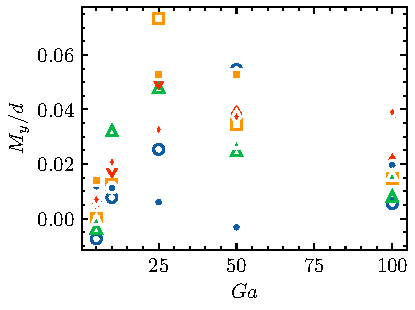
\includegraphics[height = 0.3\textwidth]{image/HOMOGENEOUS_NEW/PA/Ry.pdf}
    \caption{ Dimensionless first moment of the nearest particle pair distribution in the direction of gravity $M_y/d$. 
    ($\pmb\bigcirc$) $\phi = 0.01$; ($\pmb\triangle$) $ \phi = 0.05$; ($\pmb\square$) $\phi = 0.1$ ($\pmb\lozenge$) $\phi = 0.2$.
    The hollow symbols correspond to $\lambda = 1$, the filled symbols to $\lambda = 10$.
    % For $r<d$ we arbitrarily set $P_\text{r}^\text{th} = 1$ so that the distribution can be visualized.
    % Black symbols represent the results of \citet{zhang2023evolution} for hard sphere suspension with $\phi = 0.016,0.056,0.134,0.262$  %$\phi = 0.0168,0.0565,0.1341,0.2622$ 
    % corresponding to $\pmb\times,\pmb +, \pmb\star , \pmb\triangledown$, respectively.
    }
    \label{fig:ap:RY}
\end{figure}
%This is demonstrated by \ref{fig:ap:RY} 
%where we can see that the first moment of $P_\text{nst}$, namely
We define the first moment of $P_\text{nst}$ as
\begin{equation}
 \textbf{M} = \int_{\mathbb{R}^3} \textbf{r} P_\text{nst}(\textbf{r}) d\textbf{r}.
\end{equation}
\ref{fig:ap:RY} illustrates the projection of $\textbf{M}$ along the direction of gravity. 
The relatively small but finite values of $M_y$ indicate that $P_\text{nst}$ exhibits a nearly symmetric distribution with respect to $\theta$.
Nevertheless, this indicates that the nearest neighbor is more likely to be located in the upstream direction. 
Note that this is consistent with the findings of \citet{zhang2023evolution}.
Even though this slight asymmetry might have its importance \cite{zhang2023evolution}, we discard it in this study. 
Therefore, we choose to show only the upper part of the distribution in the following plots, (displayed in \ref{fig:Pnst_low_Ga} and \ref{fig:Pnst_high_Ga}) since qualitatively it remains the same as the lower part.  
Additionally, in the discussion below, we refer to the sphere at the origin of the graphs, located at $\textbf{x}=0$, as the \textit{test particle}.%\textit{test particle} or the \textit{test particle}. 

\subsection{Low inertia regimes}
We begin with a detailed analysis of $P_\text{nst}$ at $Ga =10$, to investigate the influence of $\lambda$ and $\phi$ on the microstructure when inertial effects are small.
\begin{figure}[h!]
    \centering
    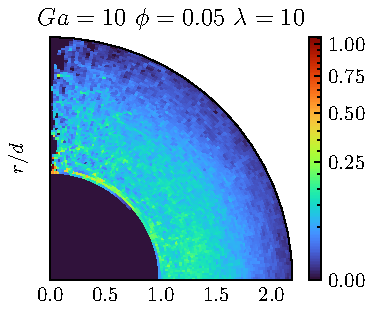
\includegraphics[height=0.21\textwidth]{image/HOMOGENEOUS_NEW/Dist/Pnst_l_10_Ga_10_PHI_0_05.pdf}
    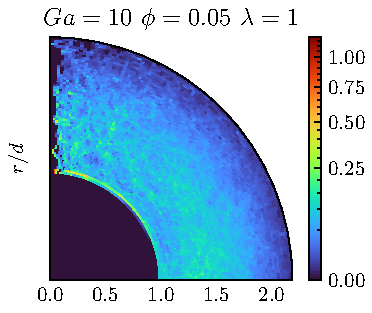
\includegraphics[height=0.21\textwidth]{image/HOMOGENEOUS_NEW/Dist/Pnst_l_1_Ga_10_PHI_0_05.pdf}
    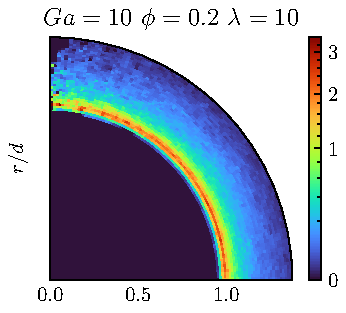
\includegraphics[height=0.21\textwidth]{image/HOMOGENEOUS_NEW/Dist/Pnst_l_10_Ga_10_PHI_0_2.pdf}
    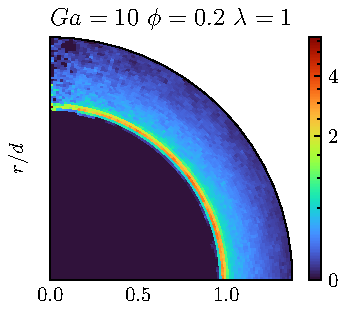
\includegraphics[height=0.21\textwidth]{image/HOMOGENEOUS_NEW/Dist/Pnst_l_1_Ga_10_PHI_0_2.pdf}
    \caption{Histogram of the probability density function, $P_\text{nst}(r,\theta)$, for low inertia $Ga = 10$.
    The color map represents the nearest pair distribution function. %the values of $P_\text{nst}$.
    The origin corresponds to the position of the \textit{test particle}.
    The dimensionless radial and azimuthal coordinates, $|\textbf{r}|/d$ and $\theta$, correspond to the nearest neighbor position.
    The vertical direction corresponds to the flow direction, which is also the axis of symmetry for $P_\text{nst}$.
    (left) Low volume fraction cases $\phi=0.05$ for $\lambda = 1,10$.
    (right) High volume fraction cases $\phi=0.2$ for $\lambda = 1,10$.
    }
    \label{fig:Pnst_low_Ga}
\end{figure}
The first observation from \ref{fig:Pnst_low_Ga} indicates that the likelihood of finding the nearest neighboring particle at an angle $\theta$ is uniform across all $\theta$.
This suggests that $P_\text{nst}$ is isotropic at these \textit{Galileo} numbers. We can observe that $P_\text{nst}$ is larger close to the \textit{test particle} ($r/d = 1$) in the high volume fraction cases than in the low volume fraction cases.
%If we compare the low volume fraction cases to the high volume fraction cases, we can observe that $P_\text{nst}$ is larger at near contact of the test particle ($r/d = 1$) in the latter case.
% For solid particles it is also common that pair distributions are more concentrated at the contact of the test particle for increasing $\phi$. 
In practice, if particles are more likely to be close to one another, it means that densely packed regions of particles are present in the flow.
This suggests that isotropic clusters, as represented in \ref{fig:scheme_clusters} (\textit{Case 2}), are likely to form in the present context. 
Regarding the effect of the viscosity ratio, $P_\text{nst}$ are very similar for both values of $\lambda$ except that for the highest volume fraction the region of highest probability is thinner for the lowest aspect ratio. 
Consequently, in this regime we find homogeneous microstructures at low $\phi$, and non-homogeneous but still isotropic microstructure (\textit{``clusters''}) at higher $\phi$. 


\subsection{High inertia regimes }
We now focus on the high inertia regimes ($Ga =80$).
In this situation, it is expected that the presence of particle wakes modify the interactions between particles \citep{yin2007}. 
\begin{figure}[h!]
    \centering
    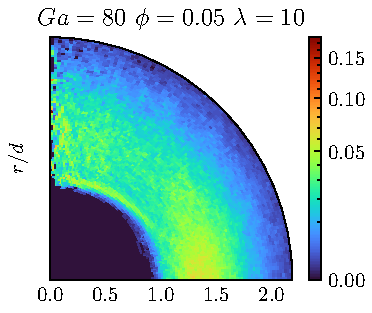
\includegraphics[height=0.205\textwidth]{image/HOMOGENEOUS_final/Dist/Pnst_l_10_Ga_80_PHI_0_05.pdf}
    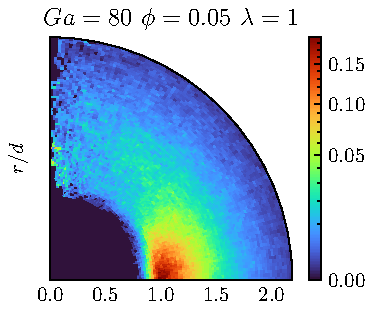
\includegraphics[height=0.205\textwidth]{image/HOMOGENEOUS_final/Dist/Pnst_l_1_Ga_80_PHI_0_05.pdf}
    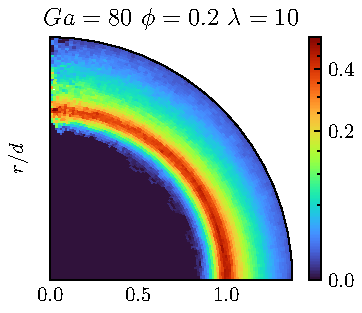
\includegraphics[height=0.205\textwidth]{image/HOMOGENEOUS_final/Dist/Pnst_l_10_Ga_80_PHI_0_2.pdf}
    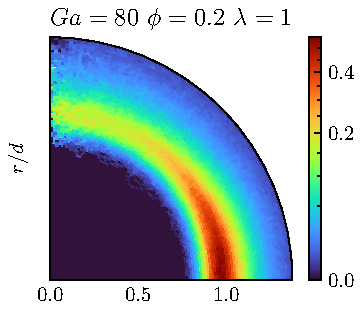
\includegraphics[height=0.205\textwidth]{image/HOMOGENEOUS_final/Dist/Pnst_l_1_Ga_80_PHI_0_2.pdf}
    \caption{Histogram of the normalized function $P_\text{nst}$ at high inertia $Ga = 80$.
    The color map represents the values of the nearest pair distribution function. %of $P_\text{nst}$.
    The origin corresponds to the position of the \textit{\textit{test particle}}.
    The dimensionless radial and azimuthal coordinates, $|\textbf{r}|/d$ and $\theta$, correspond to the nearest neighbor position.
    The vertical direction corresponds to the flow direction, which is also the axis of symmetry for $P_\text{nst}$.
    (left) Low volume fraction cases $\phi=0.05$ for $\lambda = 1,10$.
    (right) High volume fraction cases $\phi=0.2$ for $\lambda = 1,10$.}
    \label{fig:Pnst_high_Ga}
\end{figure}
%If we compare \ref{fig:Pnst_high_Ga} (right) with their counterparts from \ref{fig:Pnst_low_Ga} (right) we observe that $P^n_\text{r}$ becomes even larger at contact of the particles for $Ga=80$.
%Again, this could witness of the presence of clustering of particles. 
%In general, all $P_\text{nst}$ from \ref{fig:Pnst_high_Ga} exhibit some differences compared to the cases \ref{fig:Pnst_low_Ga}. 
%In the high inertial cases (\ref{fig:Pnst_high_Ga}), we can notice that $P_\text{nst}$ is larger on the sides of the \textit{test particle} for the iso-viscous emulsions ($\lambda = 1$).
Anisotropy in \ref{fig:Pnst_high_Ga} for $\lambda=1$ is particularly striking compared to \ref{fig:Pnst_low_Ga}. 
In the former, a higher concentration of particles is identified at $\theta \approx 0$, as seen in \ref{fig:Pnst_high_Ga}. 
A higher concentration of $P_\text{nst}$ around $\theta \approx 0$ indicates the presence of horizontal rafts of particles. 
In this case, the microstructure is non-homogeneous and anisotropic; this situation is illustrated in \ref{fig:scheme_clusters} (\textit{Case 3: ``layers''}). 
As the \textit{Galileo} number ($Ga$) increases and for low values of the viscosity ratio ($\lambda$), the probability of having neighbors on the horizontal plane of the \textit{test particle} increases. 
This leads to an increase in the anisotropy of the microstructure, which is more pronounced for low volume fractions. 
In contrast, the high-viscosity drops display an isotropic distribution of the nearest particles around the \textit{test particle}. 
This observation suggests the presence of isotropic clustering of particles.


%In comparison the high viscosity drops show an isotropic discitrbution of nearest particle around the \textit{test particle}. This could witness of the presence of isotropic clustering of particles.

%We do not observe a significant effect of the volume fraction on the anisotropy of the distribution.
%However, at this stage it remains unclear if increasing $\phi$ have a positive or negative impact on the anisotropy of the distribution. 

To illustrate the impact of $\lambda$ on the microstructure, \ref{fig:images} displays snapshots of two DNS at $\phi = 0.05$ and $Ga = 80$. 
As predicted by $P_\text{nst}$, we observe layers and particles in close contact for $\lambda = 1$, contrasting with the seemingly more evenly dispersed microstructure for $\lambda = 10$.
\begin{figure}[h!]
   \centering
   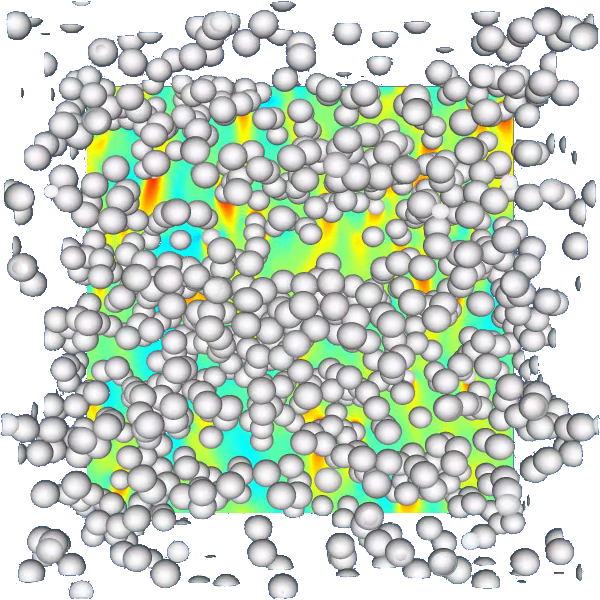
\includegraphics[width=0.45\textwidth]{image/HOMOGENEOUS_final/Ga_80_phi_005_l_1.png}
   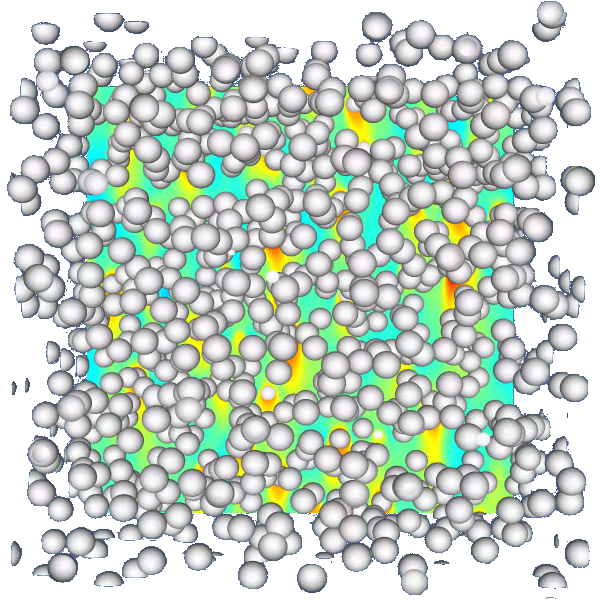
\includegraphics[width=0.45\textwidth]{image/HOMOGENEOUS_final/Ga_80_phi_005_l_10.png}
   \caption{Snapshot of a simulation at $t^* = 200$ for $\phi=0.05$ and $Ga=80$.
   Color map : values of the vertical component of the velocity, field on the vertical plane defined by the equation $z=0$. 
   (left)  $\lambda = 1$.
   (right)  $\lambda = 10$.
   }
   \label{fig:images}
\end{figure}
In fact, for $\lambda = 10$, in \ref{fig:images} (right), we can still observe horizontal rafts of droplets or droplets rising side-by-side, but this effect is not as pronounced as for $\lambda = 1$. 
Drops with high viscosity ratios maintain a significant distance between other drops, which prevents the creation of structures such as droplet layers.
% This might be because of a higher vorticity around the viscous droplets.   
% As discussed in \citet{zhang2021three}, rising pairs of spherical bubbles may reach a stable side-by-side configuration, which tends to generate horizontal clusters.
% They range of dimensionless parameters is consistent with the ones presented in this study, making this hypothesis valuable for iso-viscous emulsions. 
% In \citet{legendre2003hydrodynamic} they study the interaction of a bubble pair rising side-by-side. 
% They stipulate that for two bubbles at moderate \textit{Reynolds} number $50-100$, the interaction forces are found to be repulsive, while it is attractive or null for higher \textit{Reynolds} number. 
% In our case it is reasonable to think that such pair attraction / repulsion mechanisms might drive the clustering mechanism.
%On another note, we can observe on \ref{fig:images} (left) that the distance between the layers is roughly equal to the length of the numerical domain. 
%Indeed, only one layer of droplets is present in the domain. 
%Therefore, the current microstructure is constrained by the size of the numerical domain, it is probably not representative of the real microstructure that we would obtain in an infinite non-periodic domain. 
%Additionally, one might argue that the layers appear due to collective effects drove by the size of the box.
%Indeed, it is exactly what we observe for small number of bubbles ($N_b = 4$) rising in a periodic domain, see \citet{loisy2017}. 
%However, we might expect that horizontal layers such as the one observed in \ref{fig:images} (left) still remain for lager boxes since the number of droplets is consequent.
%In our case, the presence of horizontal raft might be the consequence of pairwise interactions mechanism, as discussed above. 
%Therefore, it is likely that that layers still appear regardless of the size of the box.
%Nevertheless, the distance between these layers is still constrained by the size of the numerical domain, despite the consequent number of droplets used here. 
%In all rigor, DNS in a larger domain with more particles would be required to evaluate the microstructure dependence on the domain size. 
%Nevertheless, due to evident numerical constrains it has not been performed in this study.  
From the present analysis of $P_\text{nst}$ and the actual microstructure presented in \ref{fig:images} we can infer that the \textit{nearest particle statistics} is able to predict features in the microstructure such as layers and clusters. 


\subsection{Nearest particle radial distribution function }

Although \ref{fig:Pnst_low_Ga} and \ref{fig:Pnst_high_Ga} give a good qualitative representation of the particle-pair azimuthal distribution, they fall short in delivering a quantitative depiction of the radial distribution.
Thus, in this section we investigate the value of the radial distribution function $P_\text{r-nst}$ defined in \ref{eq:P_r}. 
For a random isotropic distribution of hard spheres, it is possible to derive a theoretical prediction for $P_\text{nst}$ obtained in the vanishing volume fraction limit. 
Indeed, it is shown in \citet{zhang2021ensemble} that for a dilute random arrangement of particles $P_\text{nst}(r)$, reads as
\begin{equation}
    P_\text{nst}^{\phi \ll 1}(r) = n_p e^{- 8\phi\left[(r/d)^3-1\right]}.
    \label{eq:Pnst_dilute}
\end{equation}
It must be understood that this formula is accurate only at $\mathcal{O}(\phi)$; therefore, in most cases, it is not expected to be representative.
Additionally, \citet{torquato1990nearest} derived a radial distribution function for hard spheres at arbitrary volume fractions $\phi$. In our notation, this distribution can be written
\begin{equation}
    P_\text{nst}^\text{th}(r) = 
        n_p\left(e+\frac{f}{(r/d)} +\frac{g}{(r/d)^2}\right)
    e^{-\phi\left[8e\left((r/d)^3-1\right)+12 f\left((r/d)^2-1\right)+24g\left((r/d)-1\right)\right]}
    \label{eq:torquato}
\end{equation}
with, 
\begin{align*}
    && e= \frac{1+\phi}{(1-\phi)^3},
    && f= \frac{-\phi (3+\phi)}{2(1-\phi)^3},
    && g= \frac{\phi^2}{2(1-\phi)^3}.
\end{align*}
\begin{figure}
    \centering
    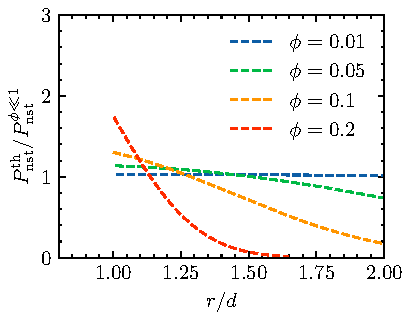
\includegraphics[height=0.3\textwidth]{image/HOMOGENEOUS_final/Dist/Theory.pdf}
    \caption{
        Theoretical prediction of $P_\text{nst}^{th}/P_\text{nst}^{\phi \ll 1}$ in terms of the dimensionless distance $r/d$ for four volume fraction $\phi$. 
    }
    \label{fig:torquato}
\end{figure}
%In both cases 
In \ref{fig:torquato} we show that $P_\text{nst}^\text{th}(r)$ predict a more concentrated nearest neighbor concentration at the contact of the \textit{test particle} ($r/d=1$) compared to the dilute random distribution $P_\text{nst}^{\phi\ll 1}(r)$. 
This effect is solely due to the consideration of the impenetrability of hard spheres. 
It should be noted that both \ref{eq:Pnst_dilute} and \ref{eq:torquato} do not consider the influence of the surrounding fluid nor the deformation of particles. 
%and may differs %from the droplet pair distribution.
In particular, for hard sphere $P_\text{nst}^\text{th} = 0$ for $r<d$ while in our case, particles might deform at contact, meaning that $P_\text{r-nst}$ is finite for certain $r<d$. 
However, using these theoretical probability density functions for comparative purposes remains valuable. 


\begin{figure}[h!]
    \centering
    % 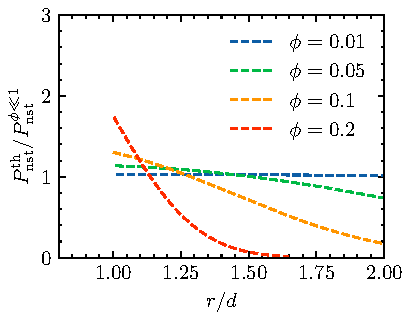
\includegraphics[height=0.3\textwidth]{image/HOMOGENEOUS_final/Dist/Theory.pdf}
    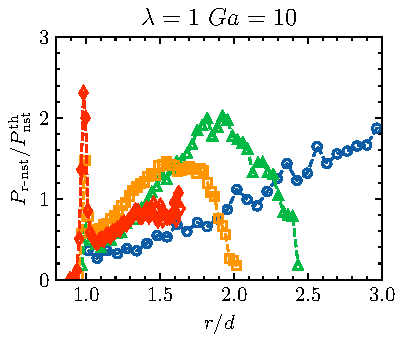
\includegraphics[height=0.3\textwidth]{image/HOMOGENEOUS_final/Dist/Pr_l_1_Ga_10.pdf}
    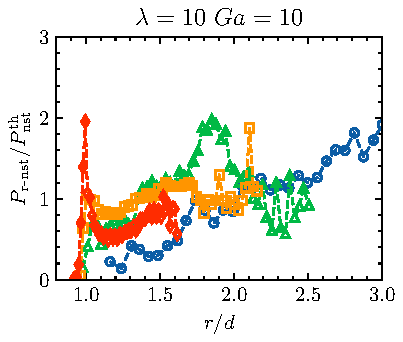
\includegraphics[height=0.3\textwidth]{image/HOMOGENEOUS_final/Dist/Pr_l_10_Ga_10.pdf}
    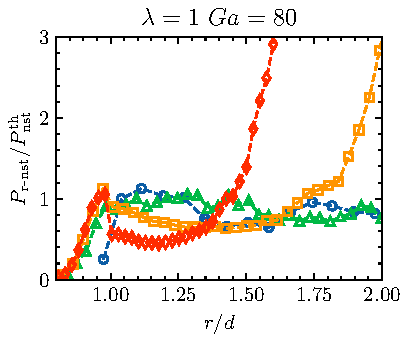
\includegraphics[height=0.3\textwidth]{image/HOMOGENEOUS_final/Dist/Pr_l_1_Ga_80.pdf}
    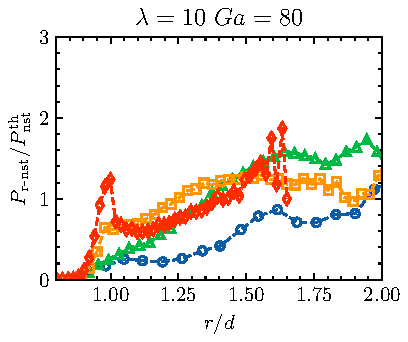
\includegraphics[height=0.3\textwidth]{image/HOMOGENEOUS_final/Dist/Pr_l_10_Ga_80.pdf}
    \caption{
    Ratio of the radial probability density functions, $P_\text{r-nst}/P_\text{nst}^\text{th}$ with $P_\text{nst}^\text{th}$ given by \ref{eq:Pnst_dilute}, as functions of the dimensionless distance $r/d$, for $Ga = 80$, $Ga =10$, $\lambda = 1$ and $\lambda = 10$.
    % (dashed lines) Theoretical prediction : $P_\text{nst}^{th}/P_\text{nst}^{\phi \ll 1}$. 
    (symbols) DNS results of $P_\text{r-nst}(r) / P_\text{nst}^{\phi \ll 1}$ with :
    ($\pmb\bigcirc$) $\phi = 0.01$; ($\pmb\triangle$) $ \phi = 0.05$; ($\pmb\square$) $\phi = 0.1$ ($\pmb\lozenge$) $\phi = 0.2$.
    For $r<d$ we arbitrarily set $P_\text{nst}^\text{th} = 1$ so that $P_\text{r-nst}$ can be visualized. 
    This, is why the ratio  $P_\text{r-nst}/P_\text{nst}^\text{th}$ may exhibit discontinuity at $r/d =1$. 
    }
    \label{fig:Pr}
\end{figure}
We plotted in \ref{fig:Pr} the ratio $P_\text{r-nst}/P_\text{nst}^\text{th}$ as functions of the dimensionless distance $r/d$.
This is particularly interesting to study since it represents the effect of fluid dynamics and particle interactions on the nearest pair distribution, given that $P_\text{nst}^\text{th}$ already accounts for the geometric effects due to finite volume fraction $\phi$. 
In \ref{fig:Pr} we display the distributions for two different viscosity ratios and multiple volume fractions. 
Let us first examine the low inertia cases displayed in \ref{fig:Pr} (top). 
It is seen that at $\phi = 0.01$ we have $P_\text{r-nst} < P_\text{nst}^\text{th}$ for roughly $r/d < 2$.
This indicates that the likelihood of finding the nearest neighbor in the vicinity of the \textit{test particle} (i.e. $r/d<2$) is less than $P_\text{nst}^\text{th}$.
In opposition, at $r/d>2$ the probability density $P_\text{r-nst}$ is higher than $P_\text{nst}^\text{th}$.
In these cases, i.e. $\phi = 0.01$ and $\lambda = 10, 1$, the maximum of $P_\text{r-nst}/P_\text{nst}^\text{th}$ is reached at $r/d \approx 3$, indicating that on average, more pairs of nearest neighbors are found with a significant distance between each other compared to the random cases. 
For comparison, the distance to the nearest neighbor in an ordered array of particles in a cubic lattice is  $\frac{1}{2}\left[4\pi/(\phi 3)\right]^{1/3} \approx 3.74$ at $\phi = 0.01$.
Additionally, it is interesting to notice that $P_\text{r-nst}/P_\text{nst}^\text{th}(r/d =1) \approx 0$ while $P_\text{nst}^\text{th}(r/d =1) = 1$ (see \ref{fig:torquato}), implying that in this regime, very few particle-particle contacts are observed. 
Overall, hydrodynamic interactions appear to maintain particles at a relatively greater distance from each other compared to the random case in the low inertia and dilute regime.
As $\phi$ increases, the maximum of $P_\text{r-nst}/P_\text{nst}^\text{th}$ is found at lower values of $r/d$. 
At $\phi = 0.2$ a local maximum is observed at $r/d = 1$ and another at $r/d = 1.5$.
This signifies that the probability of finding a nearest neighbor between the spherical shells of radius $r/d = 1$ and $r/d = 1.5$ is lower than the theoretical prediction.
In contrast, the density of finding a particle outside this area seems greater than $P_\text{nst}^\text{th}$. 
Therefore, at large $\phi$, hydrodynamic interactions seem to induce fewer neighbors at mid-distance ($1<r/d<1.5$) from \textit{test particle} than the theoretical prediction. 
At this stage, no significant differences between the cases $\lambda = 1$ and $\lambda = 10$ have been identified.

Let us now focus on the inertial cases displayed on \ref{fig:Pr} (bottom). 
For $\phi = 0.01, 0.05$ and $\lambda=1$, we observe that $P_\text{r-nst}$ is in reasonable agreement with $P_\text{nst}^\text{th}$.  
For higher volume fractions at the same $\lambda$, we observe that $P_\text{r-nst}/P_\text{nst}^\text{th} < 1$ at moderate values of $r/d$,  indicating that hydrodynamic interactions seem to repel particles from each other. 
Then, for increasing values of $r/d$, $P_\text{r-nst}/P_\text{nst}^\text{th}$ reaches surprisingly high values.  
This can be explained by the following observation. 
As demonstrated in \ref{fig:images} and \ref{fig:Pnst_high_Ga} the microstructure is highly inhomogeneous in these cases ($Ga =80$ and $\lambda =1$), specifically they exhibit clusters of particles and layered structures.
Additionally, note that the presence of clusters ultimately implies the presence of particle-free regions as $\phi$ must remain constant. 
Consequently, the likelihood for a particle to be far from its nearest neighbors is increased, as particle-free regions allow some particles to be isolated from all others by being located at the center of these regions.
Thus, this explains the high value of $P_\text{nst}^\text{th}$ at large $r/d$ in \ref{fig:Pr} (bottom-left) compared to the random distribution $P_\text{nst}^\text{th}$ which is nearly null at these values of $r/d$ (see \ref{fig:torquato}). 
In contrast, for  $\lambda = 10$ and $\phi=0.01,0.05$, it becomes evident that fewer particles are observed in close vicinity to the \textit{test particle} compared to $P_\text{nst}^\text{th}$. 
Consequently, for $Ga = 80$ and $\phi \le 0.05$, hydrodynamic interactions seem to be more significant for $\lambda=10$ than $\lambda=1$, as we observe lower values of $P_\text{r-nst}/P_\text{nst}^\text{th}$ in the close vicinity of the \textit{test particle} in the former case.
Additionally, for higher volume fraction still at $\lambda = 10$, the behavior described above where we identified very high values of $P_\text{r-nst}/P_\text{nst}^\text{th}$ at large $r/d$, cannot be observed here.
This might be because the suspension is more evenly dispersed in these cases.  
Lastly, it is clear from \ref{fig:Pr} that the particles deform at contact, as witnessed by the non-vanishing value of $P_\text{r-nst}$ for $r/d<1$.
This phenomenon is particularly pronounced for the case $Ga = 80$ and $\lambda =1$. 
This is consistent with the high values of droplet aspect ratios reported in \ref{ap:deformation} \ref{fig:chi} for this case.



To conclude these observations, we note that both the radial and azimuthal distributions were affected by the inertial effects measured by the \textit{Galileo} number. 
The major effect of high inertia is the generation of strong anisotropy in the particle pair distribution and a more important concentration of neighboring particles at $r/d < 1$. 
Furthermore, the density at contact and close contact of the \textit{test particle} is higher for increasing volume fractions as predicted by $P_\text{nst}^\text{th}$  (see \ref{fig:torquato}).
This tendency persists even though it is influenced by the particles' hydrodynamic interactions, as evidenced by \ref{fig:Pr}. 
Overall, $P_\text{nst}^\text{th}$ seems to represent $P_\text{r-nst}$ well only in the cases where $\lambda =1$, $Ga = 80$ and $\phi \le 0.05$. 
It must be concluded that, in this regime, fluid dynamics and particle interactions have the least influence on the final pair distribution, in contrast to the low inertia or viscous droplet regime ($\lambda =10$).
% as depicted by \ref{fig:torquato} and vekcrified in \ref{fig:Pr}. 
Thus, the viscosity ratio strongly impacts the microstructure, but only at high $Ga$, whereas at low $Ga$, the change in viscosity ratio has no notable impact on $P_\text{nst}$. 
% Lastly, note that \ref{eq:torquato} provides a significantly improved prediction of the radial distribution compared to $P_\text{nst}^{\phi \ll 1}$ \eqref{eq:Pnst_dilute} (see \ref{fig:Pr}). 
% Indeed, the DNS results show that $P_\text{r-nst}$ follows trends similar to $P_\text{nst}^\text{th}$ as $\phi$ increases. 
% Quantitative agreements are particularly observed for high inertia cases.

\subsection{Macroscopic modeling of the microstructure}
%Up to now we have presented visualizations of the microstructure with 2D or 1D distributions. 
%For a more concise description we would like to adopt a different approach. 
%Following \citet{zhang2023evolution} we opt to describe the microstructure using the second moment of $P_\text{nst}$ with respect to \textbf{r}, which reads
Until now, we have depicted the microstructure through 2D or 1D distributions. To provide a more succinct description, we propose a different method. 
Inspired by \citet{zhang2023evolution}, we will characterize the microstructure using the second moment of $P_\text{nst}$ with respect to $\mathbf{r}$, which is expressed as
\begin{equation}
    \textbf{R} =\frac{1}{n_p} 
    % \int_0^\infty 
    \int_{\mathbb{R}^3} 
    \textbf{rr} P_\text{nst}(\textbf{r}) d\textbf{r}.
    \label{eq:R}
\end{equation}
The tensor $\textbf{R}$ allows us to measure the mean-square distance between a particle and its nearest neighbor in the three dimensions of space.
%This second-rank tensor measures the spread of the nearest neighbor distribution in a given direction. 
It is worth noting that such a quantity is computable only because $\lim_{|\textbf{r}|\to \infty} P_\text{nst}(\textbf{r}) = 0$, which enables the integral of \ref{eq:R} to converge. 
This would not be the case for classical pair distributions, which is one of the main reasons for using the \textit{nearest particle statistics} framework. Since our objective is to measure the anisotropy of the microstructure, we are particularly interested in the deviatoric part of this tensor, namely
\begin{equation*}
    \textbf{A} = \textbf{R} - \frac{1}{3}  \text{tr}(\textbf{R}) \bm\delta.
\end{equation*}
Where $\bm\delta$ is the unit tensor and 
$\textbf{A}$ represents the likelihood of having a particle in a given direction compared to the mean radial square distance. 
Therefore, in an isotropic suspension, we have $A_{xx} = A_{yy} = 0$, where $y$ represents the coordinate aligned with gravity. 
In a situation like the one depicted in \ref{fig:images} (left), particles are more likely to have closer neighbors on the lateral sides rather than vertically positioned, hence  $A_{yy} < 0$ and $0 < A_{xx}$. 


To facilitate the understanding of the subsequent findings, it is helpful to calculate the distance $r_m$. 
This distance represents the average distance to the closest neighboring particle within a random arrangement of dilute hard spheres. 
Through direct integration of \ref{eq:Pnst_dilute}, we get
\begin{align}
    \frac{r_m^2}{d^2}
    = 
    % \frac{1}{n_p}
    \frac{1}{d^2}
    \int_{\mathbb{R}^3} r^2 P_\text{nst}^{\phi \ll 1}(\textbf{r}) d\textbf{r} 
    =  \frac{\Gamma\left({{5}\over{3}} , 8\,\phi\right)}{8^{2/3}}\frac{e^{8\phi}}{\phi^{2/3}},
    % = d^2{{4^{{{2}\over{3}}}\,\Gamma\left({{5}\over{3}} , 8\,\phi\right)
    % \,e^{8\,\phi}}\over{2^{{{10}\over{3}}}\,\phi^{{{2}\over{3}}}}}
\end{align}
where $\Gamma(z,a) = \int_a^\infty t^{z-1} e^{-t} dt$ is the upper incomplete gamma function.
\begin{figure}
  \centering
  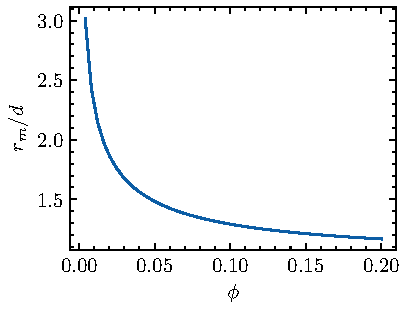
\includegraphics[height = 0.3\textwidth]{image/HOMOGENEOUS_final/PA/rm.pdf}
  \caption{Dimensionless radial distance $r_m/d$ to the nearest neighbor for a random distribution.}
  \label{fig:agee}
\end{figure}
Since the upper incomplete gamma function is relatively uncommon, we have illustrated the dimensionless distance $r_m/d$ as a function of $\phi$ in \ref{fig:agee} to aid understanding. This figure clearly shows that $r_m$ decreases as $\phi$ increases.
%Since the upper incomplete gamma function is not so common we have plotted in \ref{fig:ap:agee} the dimensionless distance $r_m/d$ in terms of $\phi$ to help comprehension. As can be seen from this figure $r_m$ is a decreasing function of $\phi$.

\begin{figure}[h!]
    \centering
    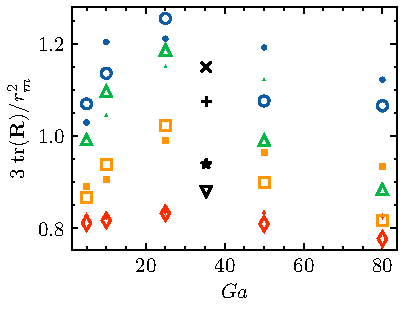
\includegraphics[height=0.3\textwidth]{image/HOMOGENEOUS_final/PA/trR.pdf}
    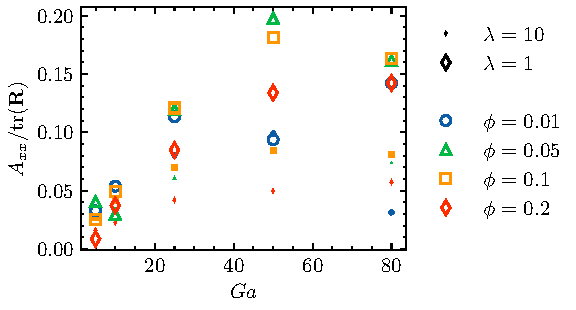
\includegraphics[height=0.3\textwidth]{image/HOMOGENEOUS_final/PA/Axx.pdf}
    \caption{
        (left) Dimensionless trace of $\textbf{R}$ as a function of the volume fraction.%Trace of the second moment of the probability density function $P_\text{nst}(\textbf{r})$ divided by the square diameter of the particles $d^2$. 
        (right) Horizontal components of the anisotropy tensor divided by the trace of $\textbf{R}$. %the second moment of the probability density function.
    ($\pmb\bigcirc$) $\phi = 0.01$; ($\pmb\triangle$) $ \phi = 0.05$; ($\pmb\square$) $\phi = 0.1$ ($\pmb\lozenge$) $\phi = 0.2$.
    The hollow symbols correspond to $\lambda = 1$, the filled symbols to $\lambda = 10$.
    % For $r<d$, we arbitrarily set $P_\text{nst}^\text{th} = 1$ so that the distribution can be visualized.
    Black symbols represent the results of \citet{zhang2023evolution} for sedimenting spherical particles with $\phi = 0.016,0.056,0.134,0.262$ and $\zeta = 2.56$. %$\phi = 0.0168,0.0565,0.1341,0.2622$ 
    Corresponding to $\pmb\times,\pmb +, \pmb\star , \pmb\triangledown$, respectively.
    }
    \label{fig:A}
\end{figure}
In \ref{fig:A} (left), the dimensionless mean square distance between nearest neighbors, represented as $3\cdot\text{tr}(\textbf{R})/r_m^2 = \textbf{R}:\bm\delta/r_m^2$, is illustrated for all configurations explored in this study. 
The simulation marked by the symbol \textcolor{col1}{$\pmb\circ$} in \ref{fig:A} (left), corresponding to parameters $\lambda = 1$, $Ga = 80$, and $\phi = 0.01$, yields a value of $\bm\delta:\textbf{R}/r_m^2 \approx 1$. 
This observation agrees with the quasi-hard-sphere distribution previously reported in this case in \ref{fig:Pr} (left).
The dependence of the mean square distance on the volume fraction is also displayed on \ref{fig:A} (left). 
We observe a decrease in $\bm\delta:\textbf{R}/r_m^2$ as $\phi$ increases, indicating that particles tend to come closer to each other on average compared to a dilute random distribution of hard spheres. 
This observation, as highlighted by \citet{zhang2023evolution}, suggests the emergence of clusters when increasing the particle volume fraction. 
Note that this trends is not due to hydrodynamic effect but rather to geometrical effect already predicted by $P_\text{nst}^\text{th}$ (see \ref{fig:torquato}). 
The dependence on the \textit{Galileo} number is non-monotonic. 
Indeed $\bm\delta:\textbf{R}/r_m^2$ increases until $Ga = 25$ and then decreases until $Ga = 80$. We also note that the distance to the nearest neighbor is not significantly affected by the viscosity ratio, particularly when dealing with high-volume fractions. 
In \ref{fig:A} (left), the symbols $\pmb\star$, $\pmb\times$, $\pmb +$, and $\pmb\triangledown$ depict the findings from the study conducted by \citet{zhang2023evolution} on the sedimentation of solid spheres in a liquid.
As observed, the value of $\textbf{R}:\bm\delta$ is, on average, closer to the mean $r_m^2$ than our simulations, but it maintains the same trend, i.e., clusters appear as the volume fraction increases.
 
\ref{fig:A} (right) illustrates the anisotropy of the microstructure. We can see on \ref{fig:A} (right) that we have $A_{xx} \ge 0$ for nearly all our cases, meaning that the emulsion is either isotropic ($A_{xx} = 0$), or exhibits a tendency towards a horizontal alignment of particles on average ($A_{xx} >0$). % or with particles that are in average more aligned horizontally ($A_{xx} >0$). 
%Moreover $A_{xx}$ increases with $Ga$ until $Ga = 50$ where we reach a maximum, and then decrease until $Ga =80$  but still remains consequent. 
Additionally, $A_{xx}$ rises with $Ga$ up to $Ga = 50$, reaching a peak, and subsequently decreases until $Ga = 80$, although it remains significant.
In agreement with the remarks of the previous section, the value of $A_{xx}$ is greater for $\lambda = 1$ and lower for  $\lambda = 10$.
Although not obvious at first, we observe a non-monotonic trend with the volume fraction. $A_{xx}$ increases up to a peak value at $\phi = 0.1$ (indicated by \textcolor{col3}{$\pmb\square$} on \ref{fig:A} (right)), but then decreases for $\phi=0.2$ (shown by the \textcolor{col4}{$\pmb\lozenge$} symbols). %$A_{xx}$ first increases up to a maximum value for $\phi =0.1$ (represented by \textcolor{col3}{$\pmb\square$} on \ref{fig:A} (right)) and then decreases for $\phi=0.2$ (represented by the \textcolor{col4}{$\pmb\lozenge$} symbols).
%Although, it is not quite obvious we observe a non-monotonic trend with the volume fraction, $A_{xx}$ first increases up to a maximum value for $\phi =0.1$ (represented by \textcolor{col3}{$\pmb\square$} on \ref{fig:A} (right)) and then decreases for $\phi=0.2$ (represented by the \textcolor{col4}{$\pmb\lozenge$} symbols). 
This implies that at a certain volume fraction, around $\phi \approx 0.1$, higher $\phi$ makes the microstructure more isotropic, while at low volume fraction ($\phi < 0.1$), increasing $\phi$ favors the side-by-side configuration.
This phenomenon of isotropization at high $\phi$ has been reported in other studies such as in \citet{seyed2021sedimentation} for sedimentation of solid particles. 
However, at high \textit{Galileo} numbers, it seems that this effect is less pronounced. 


To conclude, we classify the microstructure into four classes :
(1) The homogeneous microstructure.
(2) The non-homogeneous but isotropic microstructure with $\textbf{R}:\bm\delta > r_m^2$, or dispersed arrangement. %ordered array.
(2 bis) The non-homogeneous but isotropic microstructure with $\textbf{R}:\bm\delta < r_m^2$, or clustering. 
(3) The non-homogeneous and non-isotropic microstructure or layering ($\textbf{A}\neq \textbf{0}$). 
Each of these types is characterized by specific values of $\textbf{R}$; they are reported in \ref{tab:microstructure}. 

\begin{table}[h!]
    \caption{Microstructure classification}
    \label{tab:microstructure}
    \centering
    \begin{tabular}{|lccccc|} \hline
        Microstructure types & Homogeneous & Isotropic & \ref{fig:scheme_clusters} & $\textbf{R}:\bm\delta/r_m^2$ & $A_{xx}/tr(\textbf{R})$ \\
        Homogeneous & Yes & Yes &(\textit{Case 1}) & $ \approx 1$ & $\approx 0$ \\
        Dispersed &  No & Yes  &(\textit{Case 2}) & $ > 1$ & $\approx 0$ \\
        Clustering &  No & Yes  &(\textit{Case 2}) & $ < 1$ & $\approx 0$ \\
        Layering &    No & No  &(\textit{Case 4}) & $ - $ & $< 1$\\ \hline
    \end{tabular}
\end{table}
Additionally, to highlight the dependence of $\textbf{R}$ on $\phi$ and $Ga$, we display the values of $A_{xx}/tr(\textbf{R})$ and $\textbf{R}:\bm\delta/r_m^2$ in phase diagrams on \ref{fig:phase}.
We observe that the mean square particle distance compared to a random case decreases when increasing the volume fraction and is globally higher for viscous particles ($\lambda = 10$).
Meanwhile, the likelihood of finding the nearest neighboring particle on the horizontal is greater for $\lambda=1$ than $\lambda = 10$, and it is globally increasing with  $Ga$ and non-monotonic with $\phi$. 
We reach the configuration with the maximum anisotropy for both viscosity ratios at $Ga \approx 50$ and $\phi \approx 0.1$. 
%We conclude that 

\begin{figure}[h!]
    \centering
    \begin{tikzpicture}[scale=0.8]
        \node (img) at (0,0) {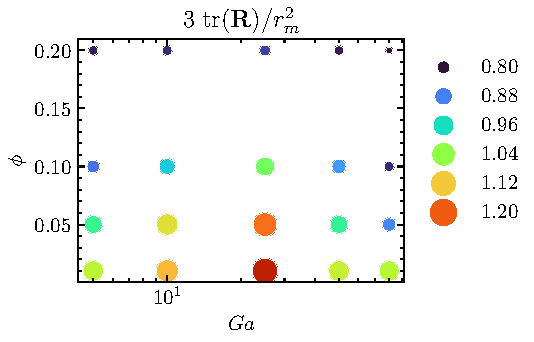
\includegraphics[height=5.5cm]{image/HOMOGENEOUS_final/PA/phase_Rtr_l_1.pdf}};
        % \draw[dashed] (10cm,-1.6) ellipse (3 and 2);
        \node (txt) at (-2,1) {Clustering};
        \node (txt) at (-1,-1.6) {Dispersed};
        \draw[dashed] ($(-1,-1.6) + (-10:3 and 2)$(P) arc
        (-10:155:3 and 2);
        \node (img) at (10.5,0) {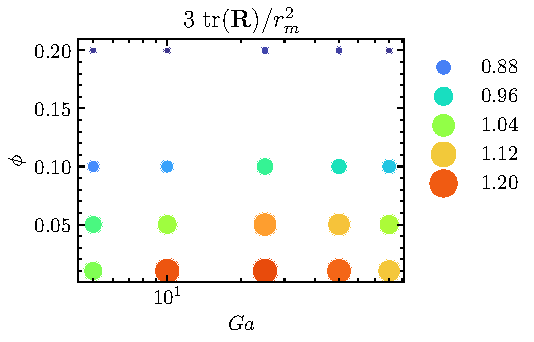
\includegraphics[height=5.5cm]{image/HOMOGENEOUS_final/PA/phase_Rtr_l_10.pdf}};
        % \draw[dashed] (10cm,-1.6) ellipse (3 and 2);
        \node (txt) at (8.5,1) {Clustering};
        \node (txt) at (10,-1.6) {Dispersed};
        \draw[dashed] ($(10,-2) + (-10:3 and 2)$(P) arc
        (-10:180:3 and 2);
    \end{tikzpicture}
    \begin{tikzpicture}[scale=0.8]
        \node (img) at (0,0) {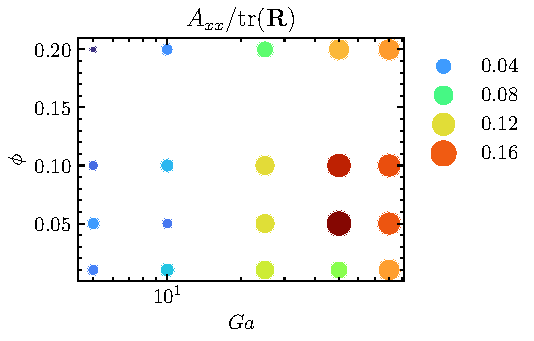
\includegraphics[height=5.5cm]{image/HOMOGENEOUS_final/PA/phase_axx_l_1.pdf}};
        \draw[dashed] (1.4,0.3) ellipse (1.5 and 2.5);
        \node (txt) at (1.4,1) {Anisotropic};
        \node (txt) at (-2,1) {Isotropic};

        \node (img) at (10.5,0) {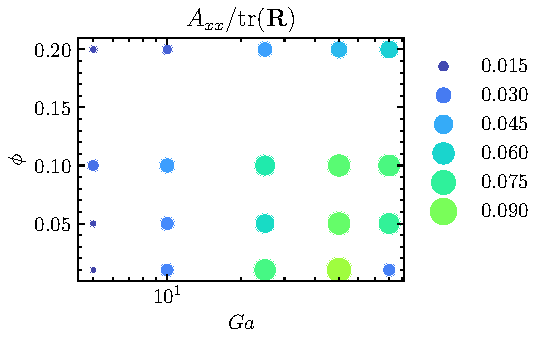
\includegraphics[height=5.5cm]{image/HOMOGENEOUS_final/PA/phase_axx_l_10.pdf}};
        % \draw[dashed] (11.7,-0.5) ellipse (0.75 and 1.75);
        % \node (txt) at (11.7,1) {Anisotropic};
        \node (txt) at (8,1) {Isotropic};
    \end{tikzpicture}
    \caption{
        (top) Phase diagram of the dimensionless mean square distance to the nearest neighbor, $\bm\delta:\textbf{R}/r_m^2$.
        (bottom) Phase diagram of the dimensionless horizontal components of the anisotropy tensor, $A_{xx}/\text{tr}(\textbf{R})$.  
        (left) Iso-viscous emulsion $\lambda = 1$.
        (right) Viscous droplets $\lambda = 10$ }
    \label{fig:phase}
\end{figure}

\subsubsection*{Discussion}
%Although, previous studies mainly focused on bubbles or solid particles, it is reasonable to compare the $\lambda = 1$ and $\lambda = 10$ simulations, to the former and the latter cases, respectively. 
%In \citet{bunner2002dynamics} they performed tri-periodic simulation of buoyant bubbles at $Re \approx 10-30$ for various $\phi$.
%They reported a preference for the bubbles to be aligned in pair.
While earlier studies primarily focused on bubbles or solid particles, it is reasonable to draw parallels between simulations with $\lambda = 1$ and $\lambda = 10$, corresponding to the former and latter scenarios, respectively. In \citet{bunner2002dynamics}, buoyant bubbles were simulated in a tri-periodic setup at Reynolds numbers around 10-30 for various volume fractions ($\phi$). The authors noted a tendency for the bubbles to align in horizontal pairs. % a finding that aligns with our observations.
This observation is consistent with what we observe in \ref{fig:phase} ($\lambda = 1$) since the anisotropy tensor is relatively high ($A_{xx} \approx 0.15$) for $Ga = 25$ (which corresponds roughly to $Re = 25$). 
% Additionally, it is seen that these layers structures are lost at lower volume fraction ($\phi = 0.01$). 
Moreover, \citet{zhang2021direct} conducted Direct Numerical Simulations (DNS) of buoyant bubbly flows within tri-periodic domains. The Reynolds numbers varied from $Re=18$ to $22.8$ across different volume fractions, $\phi$, ranging from $0.05$ to $0.2$, with a fixed Galileo number, $Ga$, of $29$. They observed the presence of anisotropic clusters for $\phi > 0.1$, while noting their absence at lower volume fractions. This observation aligns with findings depicted in \ref{fig:phase} (left), where a small decrease in the value of $A_{xx}$ may be observed for the lowest $\phi$.
%Furthermore, in \citet{zhang2021direct} they carried out DNS of buoyant bubbly flows in tri-periodic domains.
%Their \textit{Reynolds} numbers range form $Re=22.5\to 18$ for various volume fraction : $\phi = 0.05\to 0.2$ and a fixed \textit{Galileo} number of $Ga = 29$. 
%They observe anisotropic clusters for $\phi >0.1$ as well, and they report that at lower volume fraction these structures are not present. 
%It is consistent with the results reported in \ref{fig:phase} (left) where we can see that the value of $A_{xx}$ clearly decreases for lower $\phi$. 

For solid particles at $Ga = 144$, it is observed in \citet{shajahan2023inertial} that vertical rafts of particles are formed in the dilute regime ($\phi \approx 0.02$). This phenomenon was attributed to a well-defined wake around individual particles, which effectively traps neighboring particles within the wake without causing repulsion toward the sides. %This effect was explained by the presence of a more developed wake for dilute solid particles which trap neighboring particles within the wake without repulsing it on the sides. 
In our case, we notice a greater concentration of particles in the vertical directions for $\lambda = 10$ compared to $\lambda = 1$ at $Ga = 80$, as evidenced by the smaller value of $A_{xx}$ in the former case. Although not immediately apparent, this phenomenon could be attributed to similar factors, namely, the wake of the viscous drop potentially inducing fewer instances of particles aligning side-by-side and more instances of vertically stable configurations. DNS at higher $Ga$ and $\lambda$ would be necessary to confirm or not the presence of the wake trapping effect. %To conclusively confirm or refute the presence of this wake-trapping effect, it would be necessary to conduct DNS at higher $Ga$ and $\lambda$ values.
%In our case we observe more particles in the verticals directions for $\lambda = 10$ than $\lambda =1$ at $Ga =80$, since $A_{xx}$ is smaller in the former cases.
%Although it is not quite obvious it might be the consequence of the same effects, i.e., the wake of the viscous drop might induce less side-by-side configuration and more vertical nearly stable configuration. 
%DNS at higher $Ga$ and $\lambda$ would be necessary to confirm or not the presence of the wake trapping effect.
%In our case we could not observe such a phenomenon, meaning that it might arise at larger \textit{Galileo} number or that the approximation of solid particle at for $\lambda = 10$ is too coarse.
In the moderately dense regime,  $0.02 < \phi \le 0.1$  \citet{shajahan2023inertial} identified more configurations of particles situated side-by-side. 
As mentioned above, even if it is less pronounced than for $\lambda = 1$, we indeed observe that $A_{xx}$ is higher in these cases; see \ref{fig:phase} (right). 
Additionally, \citet{almeras2021statistics} carried out experiments of liquid-solid fluidized bed with spherical particles. 
Their Reynolds numbers range between $150\leq Re \leq 360$ depending on the volume fraction $0.14 \leq \phi \leq 0.42$.
It is observed that particles are most concentrated on the horizontal plane of the reference particle when $\phi = 0.14$.
If the $\lambda = 10$ cases follow the same trend, it is reasonable to expect that the probability of horizontal configurations, already predominant at $Ga =80$, will continue to increase for higher \textit{Galileo} at $\phi  \approx 0.1$.

We would like to end this comparison with the literature with the study of \citet{yin2008lattice} which compares the microstructure of suspensions of rising bubbles with suspensions of sedimenting solid particles.
%They studied two \textit{Reynolds} numbers and two volume fractions : $Re = 5,20$ and  $\phi = 0.05, 0.2$, respectively.
%It is found that :
The study encompasses two Reynolds numbers ($Re = 5, 20$) and two volume fractions ($\phi = 0.05, 0.2$). Their findings reveal that: 
\enquote{    
     microstructure in bubble
    suspensions is more anisotropic and inhomogeneous than
    solid particle suspensions of the same volume fraction and
    \textit{Reynolds} number.    
}. 
%Although we compare emulsions with varying droplets' viscosity rather than bubbles and solid particles' suspension, our conclusion regarding the anisotropy of the flow is consistent with their study.
%Additionally, it is also observed in \citet{yin2008lattice} that the microstructure shape has a clear impact on the mean rising velocity of the dispersed phase.
%Indeed, they observed that a power-law function of $(1-\phi)$ fit perfectly the rising velocity of random and isotropic suspensions, while it is not the case when the microstructure exhibit anisotropic structures. 
%Therefore, as stated in introduction, the knowledge of the microstructure shape (reported in \ref{fig:phase}), is of utmost importance in the objective of building realistic averaged models. 
While our analysis focuses on emulsions with varying droplet viscosities rather than bubbles and suspended solid particles, our findings regarding the flow anisotropy align with the study of \citet{yin2008lattice}. 



% In the following we try to explain the origin of the striking difference between $\lambda = 1$ and $\lambda = 10$ on the particle pair distribution.
% With this objective in mind, we present a meticulous analysis of the particle time of interaction as well as the particles relative averaged velocity fields. 


\section{Relaxation time of the microstructure}
\label{sec:time}
As the previous section focused solely on the geometry of the microstructure, we now provide a more comprehensive view of the timescale that drives the interaction between nearest pairs, as well as the times scale involved for the tensor $\textbf{R}(\textbf{x},t)$.

\subsection{A transport equation}
We have seen in the last section that the tensor $\textbf{R}(\textbf{x},t)$ is able to describe the geometry of the microstructure. 
To determine how this microstructure evolves in time we make use of the transport equation of $P_\text{nst}(\textbf{x},\textbf{r},t,a)$ derived in \citet{zhang2023evolution}.
As it is a rather new formalism we recall this equation here, 
\begin{equation}
    \pddt P_\text{nst}
    + \pdda P_\text{nst}
    + \pddx \cdot  (\textbf{u}^\text{nst}_p P_\text{nst})
    + \pddr \cdot  (\textbf{w}^\text{nst}_p P_\text{nst})
    = \delta(a)P(\textbf{x},\textbf{r},0,t)
    - \frac{P_\text{nst}}{\tau^\text{nst}(\textbf{x},\textbf{r},t,a)}
    \label{eq:dt_Pnst}
\end{equation}
where $\textbf{u}^\text{nst}_p$ and $w_{pn}^\text{nst}$ is conditioned average of the particle phase velocity and relative velocity, respectively, defined \ref{sec:methodo}. 
The left-hand side of \ref{eq:dt_Pnst} corresponds to the convective derivative of $P_\text{nst}$ with respect to the nearest particle statistic phase space. 
The first term on the right-hand side of \ref{eq:dt_Pnst} account for the creation of the nearest pairs, thus it is non-zero only for the age $a = 0$. 
The second term on the right-hand side is the contribution from the destruction of the nearest pairs.
Where we defined $1/\tau^\text{nst}(\textbf{x},\textbf{r},t,a)$ as the rate of destruction of pairs particles of age $a$ with relative position $\textbf{r}$.
Additionally, we define the mean rate of destruction, $1/\tau_p$, by, 
\begin{equation*}
    \frac{n_p}{\tau_p}(\textbf{x},t) = 
    \int_{0}^\infty
    \int_{\mathbb{R}^3}
    \frac{P_\text{nst} }{\tau^\text{nst}}(\textbf{x},\textbf{r},t,a)
    da d\textbf{r}. 
\end{equation*}
As we show now, $\tau_p$ is of great importance as it governs the timescale of the microstructure.

Now, let's derive an equation for $\textbf{R}(\textbf{x},t)$.
By taking the partial time derivative of \ref{eq:R}, and utilizing \ref{eq:dt_Pnst}, we obtain:
\begin{equation*}
    \pddt (n_p\textbf{R})
    + \pddx \cdot [n_p(\textbf{u}_p\textbf{R}
    + \textbf{R}^\text{Re})]
    = 
    - \frac{n_p\textbf{R}}{\tau_p}
    +n_p\textbf{B}
    + n_p\textbf{D}
    + n_p\textbf{W}
    \label{eq:dt_R}
\end{equation*}
With,
\begin{align*}
    n_p \textbf{R}^\text{Re}(\textbf{x},t)
    =
    \int_{0}^\infty
    \int_{\mathbb{R}^3}
    \textbf{rr}(\textbf{u}^\text{nst}_p - \textbf{u}_p)
    P(\textbf{x},\textbf{r},t,a)
    d\textbf{r}da,\\
    n_p \textbf{B}(\textbf{x},t)
    =
    \int_{0}^\infty
    \int_{\mathbb{R}^3}
    \textbf{rr}
    P(\textbf{x},\textbf{r},t,0)\delta(a)
    d\textbf{r}da, \\
    n_p\textbf{D}(\textbf{x},t) = 
    \int_{0}^\infty
    \int_{\mathbb{R}^3} \textbf{rr}
    \left[
        \frac{1}{\tau_p(\textbf{x},t)}
        - \frac{1}{\tau^\text{nst}(\textbf{x},\textbf{r},t,a)}
    \right]
    P_\text{nst}
    d\textbf{r}
    da,\\
    n_p \textbf{W}(\textbf{x},t) = 
    \int_{0}^\infty
    \int_{\mathbb{R}^3} \left[
        \textbf{r} \textbf{w}^\text{nst}_p
        + \textbf{w}^\text{nst}_p\textbf{r}
    \right]P_\text{nst}
    d\textbf{r}
    da.
\end{align*} 
The tensor $\textbf{R}^\text{Re}$ represent the flux due to velocity fluctuations. 
The source term $\textbf{B}$ is the averaged square relative position conditioned on the age $a=0$, meaning that it is related to the birth of the nearest particle pairs. 
In opposition to \textbf{D} which is related to the death of the particles pairs due to the presence of $\tau_p$ and $\tau_p^\text{nst}$.
Therefore, $\textbf{D}$ is the weighted mean of $\textbf{rr}$ in terms of the destruction rate fluctuation fields. 
Likewise, $\textbf{B}$ is the weighted average of $\textbf{rr}$ on the Dirac distribution $\delta(a)$. 
The latter term cancel out under the hypothesis that $1 / \tau^\text{nst}_p(\textbf{x},\textbf{r},t,a)$ is independent of age and relative position, in which case $\tau_p = \tau^\text{nst}_p$. 
Such simplification might be valid at high particle velocities fluctuation, however in our case we could not observe this independence with the DNS results.  
Lastly, the tenor $\textbf{W}(\textbf{x},t)$ is the correlation between the particles relative position and velocity.
Due to the presence of the first term on the right-hand side of \ref{eq:dt_R}, we can state that $\textbf{R}(\textbf{x},t)$ will eventually relax within time, and that the relaxation time is $\tau_p$. 
In \citet{zhang2023evolution} they demonstrate that it is also the case for the particle-fluid-particle stress tensor.
In fact, this hold true for all nearest-neighbor averaged particles quantities, since this relaxation time is related to the transport equation of $P_\text{nst}(\textbf{x},t\textbf{r},t,a)$, see \ref{eq:dt_Pnst}.
The main takeaway from \ref{eq:dt_R} is that, the microstructure as it is described by $\textbf{R}(\textbf{x},t)$, is motivated by 3 source terms, a term related to the weighted average of $\textbf{rr}$ on pair's birth and on pair's destruction, and a last one related to the particle relative velocity-position correlation. 


Since, $\textbf{R}(\textbf{x},t)$ follow a kinetic theory-like transport equation, it is interesting to discuss the possibility of implementing an equation such as \ref{eq:dt_R} in an Euler-Euler simulation framework. 
Attempting to close the source terms on the right-hand side of \ref{eq:dt_R} is very challenging. 
Instead, one could directly close $\textbf{R}(\textbf{x},t)$ based on the results of \ref{fig:A}, which are statistically steady state results of the microstructure. 
But then, how to know if the inertial effects related to the formation of the microstructure  (left hand-side of \ref{eq:dt_R}) are negligible ?
In facts, provided a relaxation time of the microstructure sufficiently small compared to the timescale of the flow, the derivatives in the right-hand side of \ref{eq:dt_R} might be negligible.
Therefore, $\textbf{R}(\textbf{x},t)$ can be expressed directly in terms of the flow parameters, provided that $\tau_p$ is smaller than the flow timescale. 
Then, the knowledge of $\textbf{R}(\textbf{x},t)$ by either solving \ref{eq:dt_R} or by obtaining direct closures laws, provides useful information for the closure terms in the Euler-Euler model.
For example, the averaged interphase momentum transfer is microstructure dependent. 
This, of course, requires having an expression for the closure terms in terms of the pair distribution function, which is not currently feasible.
Anyhow, the time $\tau_p$ is of major importance for two reasons: 
(1) it determines the timescale at which a statistically steady microstructure might be reached; 
(2) it provides useful information for the modeling of \ref{eq:dt_R}.

\subsection{Mean age of interaction}

In this paragraph we evaluate the mean rate of destruction $1/\tau_p(\textbf{x},t)$. 
It is shown in a few paragraph that the age distribution function is closely related to the mean rate of destruction. 
Therefore, let's first examine the age distribution, defined as, 
\begin{equation*}
    P_a(\textbf{x},t,a)
    = \frac{1}{n_p(\textbf{x},t)}
    \int_{\mathbb{R}^3}
    P_\text{nst}(\textbf{x},\textbf{r},t,a)
    d\textbf{r}.
\end{equation*} 
It is possible to derive an analytical formula for the age distribution, $P_a(\textbf{x},t,a)$, under the \textit{random destruction assumption} \citep{zhang2023evolution}.
This assumption state that the probability of particle pairs destruction, integrated on all position, is uncorrelated with the age of interaction.
In other worlds, we consider that any pairs of nearest neighbor can be broken apart equally likely regardless of the current age of the particle pair. 
Let us define $1/\tau_p^a(\textbf{x},t,a) = \frac{1}{n_p}\int_{\mathbb{R}^3}\tau^\text{nst} P_\text{nst}d\textbf{r}$, as the mean rate of pair destruction at age $a$, then this hypothesis state that $\tau^a_p$ is not a function of the age, such that $\tau^a_p(\textbf{x},t,a) = \tau_p(\textbf{x},t)$. 
It must be understood that $\tau^a_p$ is independent of the age, which does not imply that $\tau^\text{nst}_p$ is independent of the relative position, $\textbf{r}$.
Under this assumption, which will be shown to be valid in our dimensionless parameters range, we can derive an analytical formula for the age distribution \citep{zhang2023evolution}, namely,
\begin{align}
    P_a(\textbf{x},t, a)  
    =\frac{e^{-a/\tau_p(\textbf{x},t)}}{\tau_p(\textbf{x},t)}.
    \label{eq:Pa}
\end{align} 
We can see that the age distribution is solely function of $\tau_p(\textbf{x},t)$ and that it is normed.
Additionally, with this definition $\tau_p(\textbf{x},t)$, turns out to be the first moment of the age distribution, such that, 
\begin{equation*}
    \int_{0}^\infty
    a P_\text{a}(\textbf{x},t,a)
    da
    =\tau_p(\textbf{x},t). 
\end{equation*}
Therefore, $\textbf{R}(\textbf{x},t)$ has a relaxation time equal to the first moment of the age distribution, which can be understood as the mean rate of interaction of the particles pairs. 
In this sense it is intuitive to understand that the microstructure reach a statistically stable equilibrium after a time of the order of the mean particle interaction time. 

In \ref{fig:age_picture} (right) we display the dimensionless age distribution $P_a(\textbf{x},t,a)$ measured in our DNS, for different volume fraction, $\lambda =1$ and $Ga = 100$. 
The age is made dimensionless using the timescale, $U/d_p$ where $d_p$ is the length scale between two particles defined as $d_p = n_p^{-3}(\textbf{x},t)$, and $U$ the averaged drift velocity.
The values of the Reynolds number based on the drift velocity are given in \ref{ap:age} for all our simulations. 
It is seen that in most cases, the age distribution are rather well represented by the theoretical age distribution from \ref{eq:Pa}.
Consequently, the \textit{random destruction assumption} holds for these cases. 
\begin{figure}[h!]
    \centering
    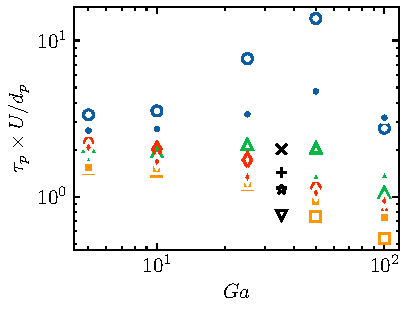
\includegraphics[height = 0.3\textwidth]{image/HOMOGENEOUS_NEW/tau_Ga.pdf}
    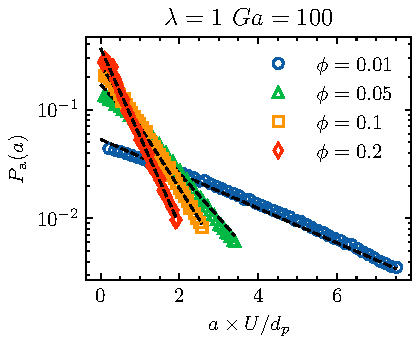
\includegraphics[height = 0.3\textwidth]{image/HOMOGENEOUS_NEW/Dist/Pa_l_1_Ga_100.pdf}
    \caption{
    (left) Mean dimensionless age $\tau_a =  \int_0^\infty aP_a(\textbf{x},t,a)da$ in terms of the \textit{Galileo} number for different volume fraction :   
    ($\pmb\bigcirc$) $\phi = 0.01$; ($\pmb\triangle$) $ \phi = 0.05$; ($\pmb\square$) $\phi = 0.1$ ($\pmb\lozenge$) $\phi = 0.2$.
    The hollow symbols correspond to $\lambda = 1$, the filled symbols to $\lambda = 10$.
    (right) Age distribution function $P_a(\textbf{x},t,a)$ in terms of the dimensionless age, for $\lambda = 1$ and  $Ga = 100$.
    (dashed lines) Theoretical age distribution, see \ref{eq:Pa}. 
    Both the age and the mean age $\tau_a$ are made dimensionless with the drift velocity $U$ and the particle length scale $d_p$.  
    Black symbols represent the DNS results of \citet{zhang2023evolution} for hard sphere suspension with $\phi = 0.0168,0.0565,0.1341,0.2622$, corresponding to the symbols : $\pmb\times, \pmb +, \pmb\star , \pmb\triangledown$, respectively.
    }
    \label{fig:age_picture}
\end{figure}
In \ref{ap:age}  we provided the age distributions but for lower inertial effects, $Ga = 10$. 
It is seen that the age distribution at $\phi = 0.01$ and $Ga = 10$, exhibits a higher density for higher ages and is smaller for small ages, compared to the random distribution.
Therefore, at low \textit{Galileo} and low $\phi$ the \textit{random destruction assumption} doesn't seem to remain valid anymore. 
The \textit{random destruction assumption} must hold true for flows with high particle velocity fluctuation compared to the mean slip velocity, which induces randomness in particle interactions \citep{zhang2023evolution}. 
It is clear that for $\phi \rightarrow 0$, the particle phase fluctuation also tends to $0$, making this condition false. 
Apart from these two cases, it is reasonable to say that \ref{eq:Pa} is well representative of the age distribution function.

In \ref{fig:age_picture} (left) we displayed the dimensionless mean age for all our numerical experiment. 
Regarding the global trend of $\tau_p$ we say that for almost all of our DNS, the time of interaction is higher for $\lambda = 1$ (hollow symbols) than for $\lambda = 10$ (filled symbols) at same $Ga$ and $\phi$.
Additionally,  $\tau_p$ seem to be well scaled by $U/d_p$ and decrease as $Ga$ and $\phi$ increase. 
We can see that $\tau_p$ clearly reaches a peak for $\phi=0.01$, $Ga=50$, $\lambda=1$.
This, may be correlated with the values of $A_{xx}$ on \ref{fig:A} which also reach a maximum for these parameters. 
Indeed, since $A_{xx}$ is rather high for these simulations, we know that particles are, on average, in a side-by-side configuration, which seems to be stable since $\tau_p$ is large.
For $\lambda = 10$ we observe a smaller $\tau_p$ and a smaller $A_{xx}$ at $\phi = 0.01$ and $Ga = 50$, indicating that, on average, the interaction are not as long whlie the microstructure is more isotropic. 
The dilute suspension of hard sphere, represented by a $\pmb\times$ symbol, seems to possess even lower $\tau_p$. 
This suggests that solid particles do not necessarily reach a stable equilibrium configuration in the dilute regime, unlike the bubble-like particles ($\lambda = 1$). 
This observation might be explained by the generation of more vorticity in the wake of solid particles, which makes the interactions less stable at these $Ga$ and $\phi$ values. 
In shot, the mean age of interaction seem to be a good way to measure the particles pairs stability, since it provide a way to measure theirs interaction time. 

As mentioned above, $\tau_p(\textbf{x},t)$ is the relaxation time of $\textbf{R}(\textbf{x},t)$. 
Consequently, the microstructure relaxation of dilute suspensions is larger, especially at $Ga = 50$, and may need a consequent amount of time to reach a steady state regime. 
This implies that the terms on the left-hands side of \ref{eq:dt_R} may not be neglected and that direct closure for the microstructure in terms of $\phi$, $Ga$ and $\lambda$ may not be achievable at these large $\tau_p$. 
In turns, this relaxation time will be reflected on the drift velocity of both phases, which is microstructure dependent. 
\begin{figure}
    \centering
    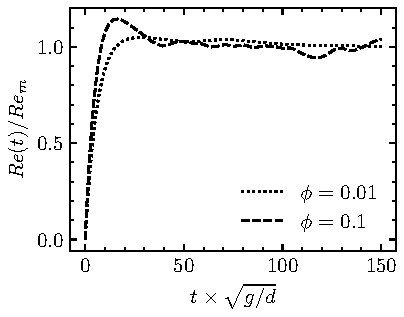
\includegraphics[height=0.325\textwidth]{image/HOMOGENEOUS_NEW/CA/Relax2.pdf}
    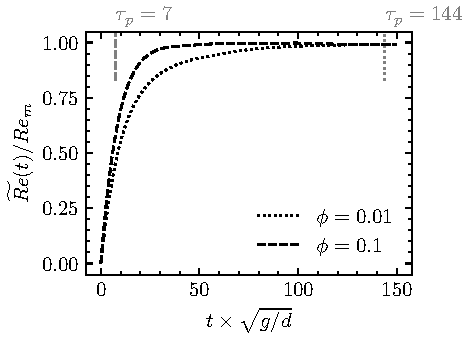
\includegraphics[height=0.35\textwidth]{image/HOMOGENEOUS_NEW/CA/Relax.pdf}
    \caption{
        (left) Average of the Reynolds number based on the instantaneous volume averaged drift velocity, $Re(t) = \rho_fU d /\mu_f$, with $U(t) = |\textbf{u}_p - \textbf{u}_f|$, divided by the mean Reynolds number $Re_m$ in terms of the dimensionless time. 
        (right) Running average of the Reynolds number $\widetilde{Re}(t)$ divided by the mean Reynolds number.
        For $\lambda = 1$ and $Ga = 50$ and two volumes fraction. 
        $\textbf{u}_p$ and $\textbf{u}_f$ are the particle and fluid phase volume averaged velocity at time $t$.
        The verticals gray lines indicate the values of $\tau_p$ all cases. 
        }
        \label{fig:relax}
\end{figure}
Indeed, in \ref{fig:relax} (right) we display the running average of the Reynolds number, based on the drift velocity, divided by the mean Reynolds number of the simulation for two values of $\phi = 0.01,0.1$ at $Ga = 50$ and $\lambda =1$. 
% It is seen that time, at which the simulation reaches a steady state regime is correlated with $\tau_p$. 
In this case we assume that two timescales are involved to bring the drift velocity to its statistically steady state regime. 
The first one is the particles' timescale, which is the time taken for a single particle to reach is terminal velocity. 
The second timescale is the time taken for the microstructure to go from random, to its steady state microstructure. 
As a matter of fact, we see that in the dilute regime ($\phi=0.01$) the rising velocity reaches its averaged value, at a time roughly equal to $100\sqrt{g/d}$ which is of the same order of magnitude than $\tau_p = 144\sqrt{g/d}$. 
On the contrary, when $\phi =0.1$ the averaged Reynolds number is indeed reached earlier ($t = 30\sqrt{g/d}$), despite the higher velocity fluctuations present in this case, see \ref{fig:relax} (left). 
The particle timescale is the same for both cases displayed \ref{fig:relax}, since only the volume fraction changes.
Additionally, the Statistical samples are supposed to be equivalent at same time since each  case posses the same number of droplets per domain. 
Thus, the changes in relaxation time is solely due to the microstructure relaxation timescale. 
Therefore, in support of the theory, $\tau_p$ seems capable of predicting the relaxation time of the microstructure among other factors such as the particle relaxation time.


The rising velocity is directly correlated to the interphase drag force in sedimentation problem \citep{jackson1997locally}. 
Therefore, in the objective of finding closure terms for the averaged models, one must perform DNS for a time longer than $\tau_p$ plus the particle timescale, to allow the microstructure to relax adequately.
Then by performing an ensemble average procedure one is able to build drag force models. 
Consequently, once established, these models will remain valid only under the condition where the timescale of the macroscopic flow significantly exceeds $\tau_p(\textbf{x},t)$ plus the particle time scale.

\subsection{Particle pairs' approach velocity}

\tb{je ne suis plus tellement sur de la pertinience de cette section}

In the next section we will be interested in the velocity fields $\textbf{w}_p^\text{nst}$ since it appear in the source term $\textbf{W}(\textbf{x},t)$, which is at the origin of the modifications of the microstructure, see \ref{eq:dt_R}. 
To give a simpler representation of $\textbf{w}_p^\text{nst}$, we first study the normal approach velocity averaged on all $\textbf{r}$, that is,  
\begin{equation*}
    w_{pn}^aP_a(\textbf{x},t,a)
    = \frac{1}{n_p(\textbf{x},t)}
    \int_{\mathbb{R}^3}
    \frac{\textbf{r}}{r} \cdot \textbf{w}^\text{nst}_p
    P_\text{nst}(\textbf{x},\textbf{r},t,a) d\textbf{r}.
\end{equation*}
In this way, $w^\text{a}_{pn}(\textbf{x},t,a)$ is the average relative normal approach velocity between the nearest pair of particles at age $a$. 
It represents the average approach velocity from one particle to its nearest neighbor, measured from the time when the particles became nearest neighbors, $a=0$.
A scheme of what $\frac{\textbf{r}}{r} \cdot \textbf{w}^\text{nst}_p$ is,  is given \ref{fig:normal_vel_picture} (right). 
\begin{figure}[h!]
    \centering
    % 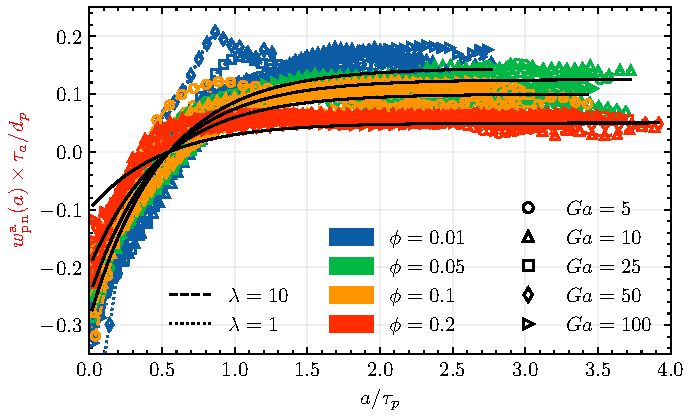
\includegraphics[height = 0.4\textwidth]{image/HOMOGENEOUS_NEW/Age_cond/uR_rel.pdf}
    % \includegraphics[height = 0.3\textwidth]{image/HOMOGENEOUS_NEW/Age_cond/r_l_10_PHI_10.pdf}
    \begin{tikzpicture}[ scale = 0.6]
        \node (img) at (-0.7\textwidth,0){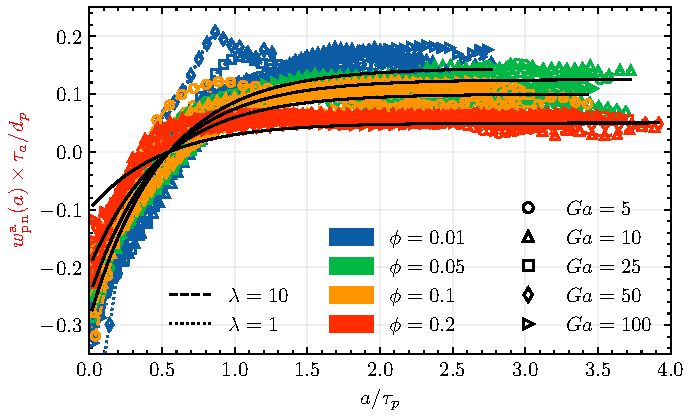
\includegraphics[height = 0.4\textwidth]{image/HOMOGENEOUS_NEW/Age_cond/uR_rel.pdf}};
        \filldraw[ gray!50!white](0,0) circle (0.5);
        \filldraw[ gray!50!white](1,3)circle (0.5);
        % \draw[fill=gray,opacity=0.2](5,-0.2)circle (0.5);
        % \draw[fill=gray,opacity=0.2](-3,2)circle (0.5);
        % \draw[fill=gray,opacity=0.2](-5,0.2)circle (0.5);
        \draw(0,0)node[right]{$\textbf{x}_i$};
        \draw[dashed](0,0)--(1,3)node[right]{$\textbf{x}_j$};
        % \draw[very thick,<-,blue](-1,0)--++(0,1)node[right]{$\bm{b}$};
        \draw[very thick,->](1,3)--++(0.9,-1.8)node[above right]{$\textbf{w}^\text{nst}(a)$};
        \draw[very thick,->,red](1,3)--++(-0.5,-1.5)node[left]{$w_{ij,n}(a)$};
        \draw[dashed](1,3)++(0.9,-1.8) -- (1,3)++(-0.5,-1.5);
        \node (ii) at (1,-1){$\textbf{w}_{ij} = \textbf{u}_j - \textbf{u}_i$};
        \node (ii) at (1,-1.6){$w_{ij,n} = \textbf{w}_{ij}\cdot \textbf{r}/|\textbf{r}|$};
        % \draw[very thick,->](0,0)--++(1,0)node[below right]{$\bm{e_x}$};
        % \draw[very thick,->](0,0)--++(0,1)node[left]{$\bm{e_y}$};
        % \draw(3,1)++(199:1)node[above left]{$\beta$} arc(199:159:1);
        % \draw(0,0)++(0:1)node[above right]{$\theta$} arc(0:20:1);
    \end{tikzpicture} 
    \caption{(left) Relative normal approach velocity between two nearest neighbors, averaged conditionally on the age of interaction.  
    The age $a$, as well as the velocity are made dimensionless  with the mean age $\tau_a$ and the length scale $d_p = n_p^{-1/3}$. 
    % The symbols represent the different \textit{Galileo} numbers, the colors the different 
    % ($\pmb\bigcirc$) $Ga=10$; ($\pmb\triangle$) $ Ga = 25$; ($\pmb\square$) $Ga = 50$ ($\pmb\lozenge$) $Ga =100$.
    % The colors represent the different volume fractions, (blue) $\phi =0.01$, (green) $\phi = 0.05$ (organ) $\phi=0.1$ (red) $\phi = 0.2$. 
    % The white symbols correspond to $\lambda = 1$, and black symbols to $\lambda = 10$. 
    (right)
    Scheme of two nearest neighbors with their position $\textbf{x}_i$ and $\textbf{x}_j$, velocities $\textbf{u}_{i}$ and $\textbf{u}_j$, relative velocity $\textbf{w}_{ij}$ and normal relative velocity $w^{ij,n}$. 
    }
    \label{fig:normal_vel_picture}
\end{figure}
The approach velocity $w_{pn}^a(\textbf{x},t,a)$ for all the DNS carried in this work is displayed \ref{fig:normal_vel_picture} (left). 
The x-axis is made dimensionless with the averaged time of interaction, $\tau_p$, and the y-axis is scaled with the velocity scale $d_p /\tau_p$. 
At  early age we observe that $w_{pn}^a<0$.
Then it eventually reaches zero for  $a \approx 0.5\tau_p$.
After this time $w_{pn}^a>0$ and remains constant with respect to $a$. 
Hence, on average, particles approach each other at early ages ($w_{pn}^a<0$), and then they move apart for $a > \tau_p$ with a constant average velocity.

Two important features are identified from \ref{fig:normal_vel_picture} (left).
First, all curves are roughly similar, even if we can see slight differences in magnitude for the different $\phi$. 
Thus, regardless of the flow parameters, $w_{pn}^a(\textbf{x},t,a)$ scale roughly as $d_p /\tau_p$. 
Second,  $w_{pn}^a(\textbf{x},t,a)$ seems to relax for age, $a > \tau_p$, to reaches a constant value. 
% Consequently, it seems that $\tau_p$ is also the relaxation time for the particles' relative normal approach velocity. 
Consequently, we demonstrated that $\tau_p$ and $d_p$ were the correct time and length scale which govern the inter particle scale kinematic, and that $\tau_p$ is also the relaxation time of $w_{pn}^a(\textbf{x},t,a)$. 
% It is clear that all nearest averaged property will be also subject to a relaxation time $\tau_p$, this in fact comes from the structure of the nearest particle averaged probability transport equation (\ref{eq:dt_Pnst}) which makes appear this relaxation time. 
In general, we believe that $w_{pn}^a(\textbf{x},t,a)$ might be useful for the future studies aiming to construct models based on the relative velocity between particles \citep{rao2008introduction}. 




\section{Inter-particle scale relative kinematic}
\label{sec:velocity}

In \ref{sec:microstructure} we have investigated the microstructure geometry, 
in \ref{sec:time} we have seen that the timescale governing both, the microstructure evolution and the particles pair relative velocity is $\tau_p$.   
We now give a visual representation of the nearest pair relative velocity in space to better understand how the relative kinematic behave.  
To that end we compute the nearest relative velocity and age, averaged on all ages, that is,
\begin{align*}
    \textbf{w}^\text{r}_pP_r(\textbf{x},\textbf{r},t)
    =\int_0^\infty \textbf{w}^\text{nst}_pP_\text{nst}(\textbf{x},\textbf{r},t,a) da,\\
    a^rP_r(\textbf{x},\textbf{r},t)
    =\int_0^\infty a P_\text{nst}(\textbf{x},\textbf{r},t,a) da.
\end{align*}
The superscript $^\text{r}$ indicate that the quantity $\textbf{w}^\text{r}_p$ and $a^r$ is conditioned on the relative position \textbf{r} only.
As will be demonstrated, having a good estimation of these velocities and ages mean fields allows one to reconstruct the history of the particles' kinematic interactions. 
To be able to visualize
$\textbf{w}^\text{r}_p(\textbf{x},\textbf{r},t)$
and 
$a^r(\textbf{x},\textbf{r},t)$
on 2D plots we consider an axis symmetry along the vertical axis, and average the values of 
$\textbf{w}^\text{r}_p(\textbf{x},\textbf{r},t)$
and $a^r(\textbf{x},\textbf{r},t)$
on the polar coordinate, as it has been done for $P_\text{nst}$ in \ref{sec:microstructure}. 
However, unlike in \ref{sec:microstructure} we do not assume symmetry with respect to the horizontal plane. 

\subsubsection*{Impact of the inertial effects}

The first effect that we study is the impact of the inertial effects on the particles relative kinematic.  
In \ref{fig:Why_Ga_matter} we display the velocity fields $\textbf{w}_p^r$ represented by the arrows that are colored by the mean dimensionless age $a^r$.  
On the left panel, we observe a low inertial case ($Ga = 10$), while on the right panel, we display a highly inertial case ($Ga=100$), both for $\lambda =1$ and $\phi=0.05$.
\begin{figure}[h!]
    \centering
    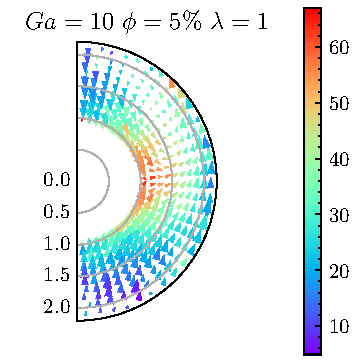
\includegraphics[height=0.35\textwidth]{image/HOMOGENEOUS_NEW/Dist/U_rel_l_1_Ga_10_PHI_5.pdf}
    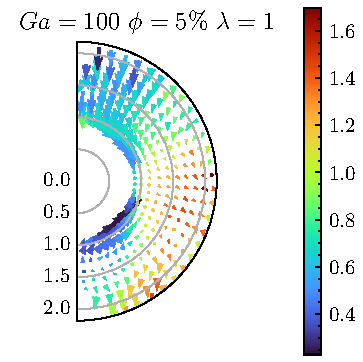
\includegraphics[height=0.35\textwidth]{image/HOMOGENEOUS_NEW/Dist/U_rel_l_1_Ga_100_PHI_5.pdf}
    % \begin{tikzpicture}[scale=0.8]
    %     \filldraw[ gray!50!white](0,0) circle (0.5);
    %     \filldraw[ gray!50!white](1,3)circle (0.5);
    %     \filldraw[ gray!50!white](-0.2,3.5)circle (0.5);
    %     % \draw[fill=gray,opacity=0.2](5,-0.2)circle (0.5);
    %     % \draw[fill=gray,opacity=0.2](-3,2)circle (0.5);
    %     % \draw[fill=gray,opacity=0.2](-5,0.2)circle (0.5);
    %     \draw(0,0)node[right]{$p_1, \; \textbf{x} = 0 $};
    %     \draw[dashed](0,0)--(1,3)node[right]{$p_2, \;\textbf{x}+\textbf{r}$};
    %     \draw[dashed](-0.2,3.5)node[right]{$p_3$};
    % \end{tikzpicture} 
    % 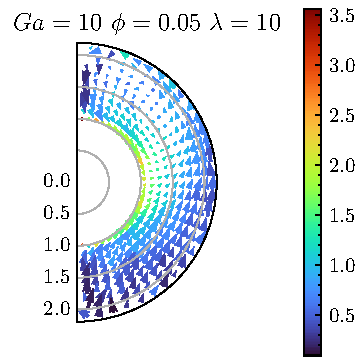
\includegraphics[height=0.35\textwidth]{image/HOMOGENEOUS_NEW/Dist/U_rel_l_10_Ga_10_PHI_5.pdf}
    % 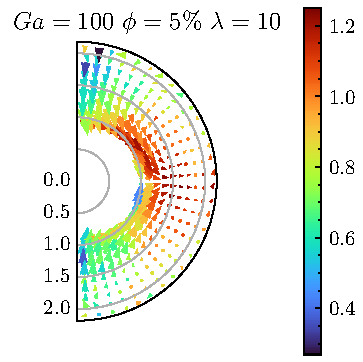
\includegraphics[height=0.35\textwidth]{image/HOMOGENEOUS_NEW/Dist/U_rel_l_10_Ga_100_PHI_5.pdf}
    \caption{
         Quiver plots of the relative averaged velocity field $\textbf{w}^\text{r}(\textbf{x},\textbf{r},t)$ colored by the averaged dimensionless age $a^r(\textbf{x},\textbf{r},t)$ for $\phi = 0.05$ and $\lambda +1$.
         (left) $Ga = 10$ (right) $Ga =100$. }
    \label{fig:Why_Ga_matter}
\end{figure}

The first aspect that we would like to clarify is the non fore-aft symmetry of the velocity fields $\textbf{w}_p^\text{nst}$ with respect to the horizontal plane. 
Indeed, in plots display on \ref{fig:Why_Ga_matter} we remark that the $\textbf{w}_p^\text{nst}$ exhibit a clear asymmetry with respect to the horizontal plane.
This is explained by the non commutativity of the function $h_{ij}$ in the indices $i$ and $j$ in \ref{eq:q_nstij}, as a result $\textbf{w}_p^r(\textbf{x},t,r,\theta) \neq \textbf{w}_p^r(\textbf{x},t,r,-\theta)$. 
Indeed, as it is depicted on \ref{fig:diagram_asym}, in the cases were the neighboring nearest particle is far from the test particle, the chance for this particle to have another nearest neighbor which is closer is high. 
Thus, the nearest neighbor of the nearest neighbor of the test particle, is not necessarily the test particle. 
This induces asymmetry in the nearest neighbor statistics. 
That explains why the plots on \ref{fig:Why_Ga_matter} are not symmetrical when we observe the fields at sufficiently large distance $|\textbf{r}|$. 
Note that this asymmetry would not be present if we had considered classic particle pair average as it is done in \cite{shajahan2023inertial}. 
To summaries, in the situation where we observe $\textbf{w}_p^r$ for large $|\textbf{r}|$ the test particle can be considered as being \textit{isolated}, as its nearest neighbor is at a large distance $|\textbf{r}|$ from the test particle. 
Additionally, the nearest neighboring particle, if located far enough, has 
potentially a nearest neighbor that is closer than the test sphere, as explained on \ref{fig:diagram_asym}. 
Consequently, provided that the nearest neighbor of the test sphere is far enough, we can be sure that on average it approaches a pair of particles or more, that are packed together. 

\begin{figure}[h!]
    \centering
    \hfill
    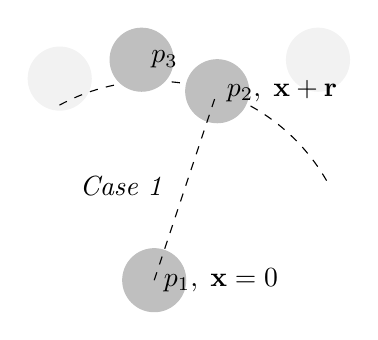
\begin{tikzpicture}[scale=0.8]
        \filldraw[ gray!10!white](+2.6,3.5)circle (0.5);
        \filldraw[ gray!10!white](-1.5,3.2)circle (0.5);
        \draw[dashed](30:3.16) arc (30:120:3.16);
        \filldraw[ gray!50!white](0,0) circle (0.5);
        \filldraw[ gray!50!white](1,3)circle (0.5);
        \filldraw[ gray!50!white](-0.2,3.5)circle (0.5);
        \draw(0,0)node[right]{$p_1, \; \textbf{x} = 0 $};
        \draw[dashed](0,0)--(1,3)node[right]{$p_2, \;\textbf{x}+\textbf{r}$};
        \draw[dashed](-0.2,3.5)node[right]{$p_3$};
        \node[ultra thick] (title) at (-0.5,1.5) {\textit{Case 1}};
    \end{tikzpicture} 
    \hfill
    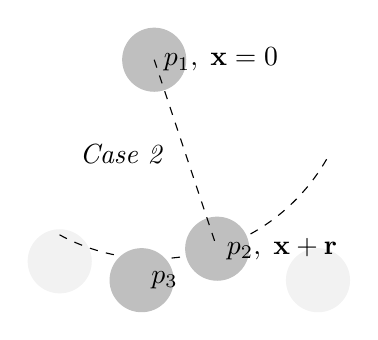
\begin{tikzpicture}[rotate=180, xscale=-0.8,yscale=0.8]
        \filldraw[ gray!10!white](+2.6,3.5)circle (0.5);
        \filldraw[ gray!10!white](-1.5,3.2)circle (0.5);
        \draw[dashed](30:3.16) arc (30:120:3.16);
        \filldraw[ gray!50!white](0,0) circle (0.5);
        \filldraw[ gray!50!white](1,3)circle (0.5);
        \filldraw[ gray!50!white](-0.2,3.5)circle (0.5);
        \draw(0,0)node[right]{$p_1, \; \textbf{x} = 0 $};
        \draw[dashed](0,0)--(1,3)node[right]{$p_2, \;\textbf{x}+\textbf{r}$};
        \draw[dashed](-0.2,3.5)node[right]{$p_3$};
        \node[ultra thick] (title) at (-0.5,1.5) {\textit{Case 2}};
    \end{tikzpicture} 
    \hfill
    % \begin{tikzpicture}[scale=0.8]
    %     \filldraw[ gray!10!white](+2.6,3.5)circle (0.5);
    %     \filldraw[ gray!10!white](-1.5,3.2)circle (0.5);
    %     \draw[dashed](-30:3.16) arc (-30:-120:3.16);
    %     \filldraw[ gray!50!white](0,0) circle (0.5);
    %     \filldraw[ gray!50!white](1,-3)circle (0.5);
    %     % \filldraw[ gray!20!white](-1.4,-3.3)circle (0.5);
    %     \filldraw[ gray!50!white](-0.2,-3.5)circle (0.5);
    %     % \draw[fill=gray,opacity=0.2](5,-0.2)circle (0.5);
    %     % \draw[fill=gray,opacity=0.2](-3,2)circle (0.5);
    %     % \draw[fill=gray,opacity=0.2](-5,0.2)circle (0.5);
    %     \draw(0,0)node[right]{$p_1, \; \textbf{x} = 0 $};
    %     \draw[dashed](0,0)--(1,-3)node[right]{$p_2, \;\textbf{x}+\textbf{r}$};
    %     \draw[dashed](-0.2,-3.5)node[right]{$p_3$};
    %     \node[ultra thick] (title) at (-0.5,-1.5) {$Case\; 2$};
    % \end{tikzpicture} 
    \caption{
        Diagram that highlights the asymmetry of the nearest pair statistic when the nearest neighbor is relatively far from the test particle.
        (\textit{Case 1}) Particle $p_1$ with  its nearest neighbor, $p_2$, located at the \underline{top} of it. 
        (\textit{Case 2}) Particle $p_1$ with  its nearest neighbor, $p_2$, located at the \underline{bottom} of it. 
        (\textit{Case 1} and \textit{2})
        In these situations the particle $p_2$ located at $\textbf{x} + \textbf{r}$, is the nearest neighbor of the particle $p_1$ located at $\textbf{x}$. 
        Since $|\textbf{r}|/d$ is assumed to be large, the nearest neighbor of the particle $p_2$ is more likely to be another nearest neighbor than $p_1$ such as the particle $p_3$, which is closer.
        This is due to the rapid decay of $P_\text{nst}$ for large $|\textbf{r}|/d$, see \ref{fig:Pnst_high_Ga}. 
        In these cases the nearest neighbor of $p_1$ is $p_2$, but the contrary is not true, inducing asymmetry in the statistics.  
    }
    \label{fig:diagram_asym}
\end{figure}

Now that this issue has been clarified, we can proceed to interpret the plots in \ref{fig:Why_Ga_matter}.
The beginning of the interactions happen at the early ages, meaning in the dark blue areas in  \ref{fig:Why_Ga_matter}, which are located on the top or bottom of the particle of reference.
The ending of the interactions corresponds to the greater ages, which are represented by the red areas. 
As shown by \ref{fig:Why_Ga_matter} (left), at low \textit{Galileo} number the nearest particle has a tendency to come from the top or bottom and leave through the sides. 
If the nearest particle is at a reasonable distance $|\textbf{r}| < 1.5d$ on the sides of the test particle, we can see that the vertical relative velocity is on average null, but positive in the radial component.
In this area, the age is at its maximum (dark red zone), therefore the interaction come to an end, meaning that the nearest particles get replace by another. 
Note that for the particles at a larger distance of the test particle, say $|\textbf{r}|>2$, have an averaged positive vertical relative velocity. 
As discussed above, in this situation the neighbor on the side is more likely to be closer to another particle. 
Consequently, if the test particle is isolated, with neighboring particles sufficiently far on the side, it will rise on average with a lower velocity than the latter particles.
Thus, particles at contact  seems to get apart because of the non-null radial velocity, and particle at distance seems to get apart because of the non-null vertical velocity.  
Consequently, on average the side-by-side configuration is not stable in this case, which partly explains why the particle distribution doesn't form any layer or such oriented microstructure at these $Ga$.   

% A plausible explanation for this phenomenon is that the leading particle accelerate the trailing particle with its wake on a first stage. 
% Then, the trailing particle arise to the same altitude as the leading particle, but still goes faster than the leading particle due to the acceleration provided by the wake of the latter particle.
% If the particles get in contact then the interaction duration seem to last longer, and the particles might even get trap in a small stagnation zone on the side of the particles.


For high \textit{Galileo} number, see \ref{fig:Why_Ga_matter} (right), the relative averaged velocity is nearly null on the sides and below the test particle. 
It is a statistical representation, meaning that, $\textbf{w}_p^r = 0$, just witnesses of the fact that the particles' relative velocity are not correlated with the relative position in this area. 
Thus, it is hard to say if the area where $\textbf{w}_p^r = 0$ corresponds to actual stagnation zones where both particles are in equilibrium, or if the relative velocity is just not correlated. 
Additionally, the particles at a large distance on the top of the test particle have a downward velocity. 
Meaning that if the test sphere is isolated and approach one or several  particles on the top of it (see \ref{fig:diagram_asym} (\textit{Case 1})), it will eventually catch up the latter particles. 
On the contrary, if the particle is isolated and that the nearest neighbor is at the bottom (see \ref{fig:diagram_asym} (\textit{Case 2})), the velocity is either pointing downward, or it is not correlated with the position, as indicated by the magnitude of $\textbf{w}_p^r$. 
A plausible explanation for this phenomenon is that the reference particle, when being isolated, goes faster than the potentially packed nearest neighbor.
Therefore, the test sphere can either catch up with the nearest particle if it is above, or move further away from it if it is below.
Also, it is interesting to notice that in this case the particles at near contact on the bottom of the test particles results from early interaction, denoted by the dark blue zone. 
It can be interpreted as follows : since 
initial time of interaction is on average low in this zone, it does mean that particles replace an old nearest neighbor that where at near contact of the test particles. 
Thus, in this case the nearest neighbor reaches the test sphere which were rising slowly because of a potentially close neighbor. 

Ultimately, the fields $\textbf{w}^r_p(\textbf{x},\textbf{r}, a)$ provide a quantitative averaged representation of what is known as the \textit{Drafting Kissing Tumbling} \citep{fortes1987nonlinear} mechanism. 
Indeed, in both case particles eventually approach from the verticals (\textit{Drafting}), nearly touch each other (\textit{Kissing}), and leave through the sides (\textit{Tumbling}). 
Statistically, the \textit{Tumbling} part is not present in the high inertial case, which  explains the creation of anisotropic structures or more stable side-by-side configurations. 
For bubble pair interactions \citet{zhang2021three} observed such DKT behavior.
They also reported side-by-side stable configuration of pairs. 
However, at same \textit{Galileo} than  \citet{zhang2021three} ($Ga = 10$) we were not able to identify this pair mechanism. 


To support the deduction made above, we displayed in \ref{fig:unst_ga} the absolute conditioned averaged center of mass velocity of the test sphere, defined as,
\begin{equation*}
    \textbf{u}^\text{r}_p(\textbf{x},\textbf{r},t)  
    =
    \frac{1}{P_r(\textbf{x},\textbf{r},t)}
    \int_0^\infty \textbf{u}^\text{nst}_pP_\text{nst}(\textbf{x},\textbf{r},t,a) da
\end{equation*}
In \ref{fig:unst_ga} (left) we clearly see that the magnitude of the test particle's vertical velocity is higher than the particle phase vertical velocity $\textbf{u}_p$ when the nearest neighbor is at near contact to the test particle, either above or below.
\begin{figure}[h!]
    \centering
    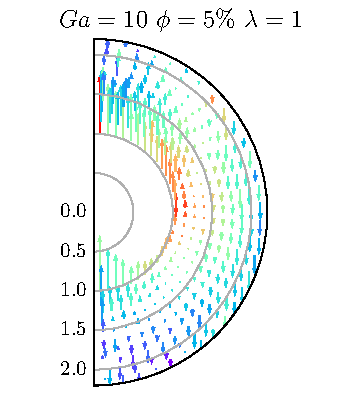
\includegraphics[height=0.35\textwidth]{image/HOMOGENEOUS_NEW/Dist/U_l_1_Ga_10_PHI_5.pdf}
    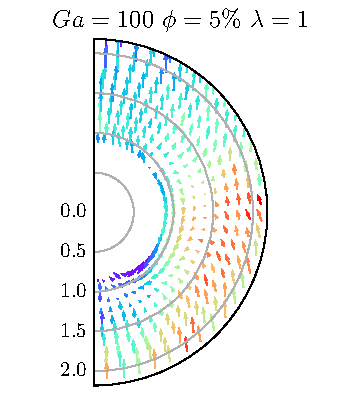
\includegraphics[height=0.35\textwidth]{image/HOMOGENEOUS_NEW/Dist/U_l_1_Ga_100_PHI_5.pdf}
    \caption{
         Quiver plots of the conditioned particle velocity field $\textbf{u}^\text{r}(\textbf{x},\textbf{r},t)$ colored by the averaged dimensionless vertical velocity difference : $(\textbf{u}^\text{r} - \textbf{u}_p )/ \textbf{u}_p$, for $\lambda = 1$ and $\phi = 0.05$. 
         (left) Low \textit{Galileo} number $Ga = 10$.
        (right) High \textit{Galileo} number $Ga = 100$.
         }
    \label{fig:unst_ga}
\end{figure}
When the nearest neighbor is at large distance of the test particle, its average velocity is lower than $\textbf{u}_p$. 
At high inertia however, the test particle velocity is higher when being isolated than with its neighbor at near contact. 
Additionally, we can see that when the particle is on the side at near contact or below, the test sphere's velocity  is lower than the mean. 
In brief in the case of $Ga = 10$ it seems that isolated particles goes slower than close neighbors packed together. 
While at higher \textit{Galileo} number it is the opposite, we observe that isolated particles  goes faster than packed neighbor. 


\subsubsection*{The volume fraction dependency}
As it has been observed in \ref{fig:A} the effect of increasing $\phi$ is that it makes the particle distribution slightly more isotropic for $\phi >0.1$. 
\begin{figure}[h!]
    \centering
    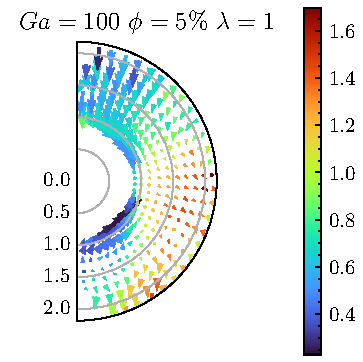
\includegraphics[height=0.35\textwidth]{image/HOMOGENEOUS_NEW/Dist/U_rel_l_1_Ga_100_PHI_5.pdf}
    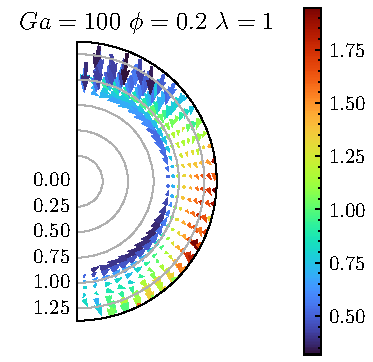
\includegraphics[height=0.35\textwidth]{image/HOMOGENEOUS_NEW/Dist/U_rel_l_1_Ga_100_PHI_20.pdf}
    % 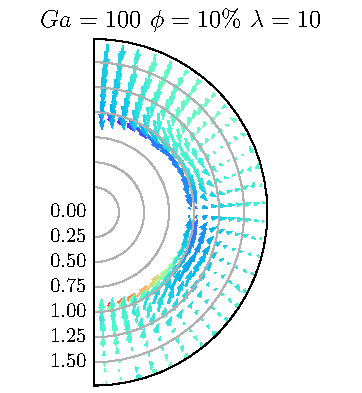
\includegraphics[height=0.35\textwidth]{image/HOMOGENEOUS_NEW/Dist/U_rel_l_10_Ga_100_PHI_10.pdf}
    % 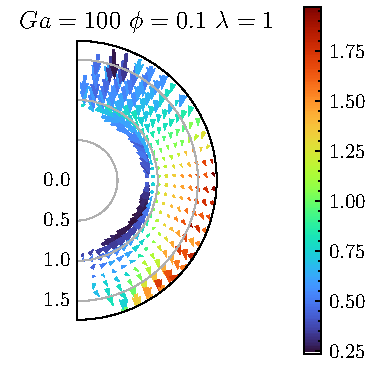
\includegraphics[height=0.35\textwidth]{image/HOMOGENEOUS_NEW/Dist/U_rel_l_1_Ga_100_PHI_10.pdf}
    \caption{Quiver plots of the relative averaged velocity field $\textbf{w}^\text{r}(\textbf{x},\textbf{r},t)$ colored by the averaged dimensionless age $a^r(\textbf{x},\textbf{r},t)$, for $Ga = 100$ and $\lambda = 1$. 
    (left) Low \textit{Galileo} number $\phi = 0.05$.
    (right) High \textit{Galileo} number $\phi = 0.2$. }
    \label{fig:Why_Phi_matter}
\end{figure}
In \ref{fig:Why_Phi_matter} we expose two situations with various volume fractions. 
In both graph we observe the same trend, despite the changes in length scales, which are due to the variations in volume fraction. 
Indeed, the stagnation zones with dark red color and the particle resulting from short interactions, dark blue color, are located approximately at the same location. 
We still observe the fore-aft asymmetry with respect to the horizontal plane, as it was discussed above. 
For other $\lambda$ and $Ga$ no particular differences could be observed with varying $\phi$. 
Overall, even if small differences might be present, the change in volume fraction doesn't seem to affect the relative kinematic of interaction between particles. 

\subsubsection*{Influence of the viscosity ratio}

Lastly, we turn our attention to the effect of the viscosity ratio on pair relative kinematic.
The question that we are trying to answer is : why does a smaller viscosity ratio increase the anisotropy of the tensor $\textbf{R}(\textbf{x},t)$ as it is shown in \ref{fig:A}. 
With this objective in mind, we compare two cases at $Ga = 100$ and $\phi =0.05$, where we observe a clear difference between the distributions (see \ref{fig:Pnst_high_Ga}) between $\lambda = 1$ and $\lambda = 10$.
\begin{figure}[h!]
    \centering
    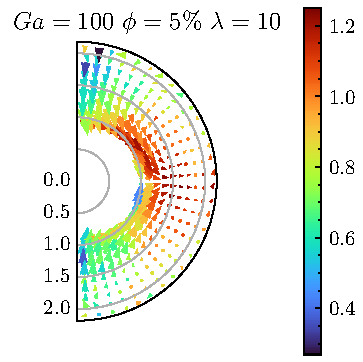
\includegraphics[height=0.35\textwidth]{image/HOMOGENEOUS_NEW/Dist/U_rel_l_10_Ga_100_PHI_5.pdf}
    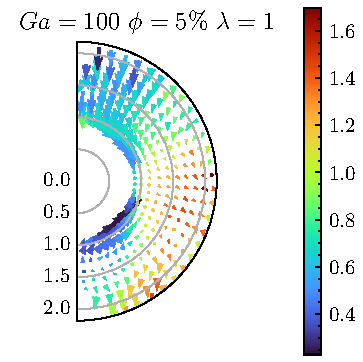
\includegraphics[height=0.35\textwidth]{image/HOMOGENEOUS_NEW/Dist/U_rel_l_1_Ga_100_PHI_5.pdf}
    % 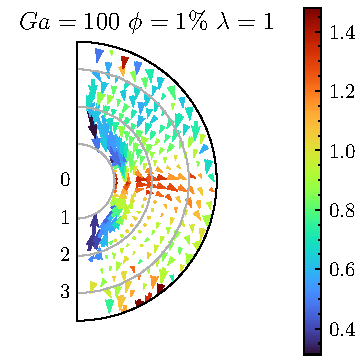
\includegraphics[height=0.35\textwidth]{image/HOMOGENEOUS_NEW/Dist/U_rel_l_1_Ga_100_PHI_1.pdf}
    % 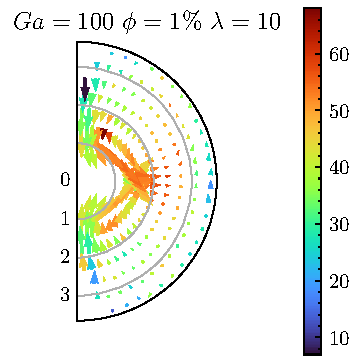
\includegraphics[height=0.35\textwidth]{image/HOMOGENEOUS_NEW/Dist/U_rel_l_10_Ga_100_PHI_1.pdf}
    \caption{Quiver plots of the relative averaged velocity field $\textbf{w}^\text{r}(\textbf{x},\textbf{r},t)$ colored by the averaged dimensionless age $a^r(\textbf{x},\textbf{r},t)$, for $\phi = 0.05$ and $Ga = 100$. 
    (left) High viscosity ratio $\lambda = 10$.
    (right) Low viscosity ratio, $\lambda = 1$. }
    \label{fig:Why_l_matter}
\end{figure}
As in the previous cases, it is clear that for both cases in \ref{fig:Why_l_matter} the neighboring particle approach on the vertical direction and end up its course on the sides.
As discussed previously, the case on \ref{fig:Why_l_matter} (right) exhibit a clear stagnation zone and asymmetry on a vertical plane. 
On the other hand for $\lambda =10$ the relative velocity on the vicinity of the particle seem to be on average positive in the radial direction. 
In addition, The asymmetry aforementioned is not present in this case. 
As discussed in the previous paragraph, and explained by \ref{fig:diagram_asym}, the presence of the skew asymmetry in the fields $\textbf{w}_p^\text{r}$ about horizontal plane, witnesses for interactions of the isolated particles clusters of particles.
The absence of such asymmetry implies the absence of such interactions, indicating that the particles are more evenly spread. 

As before, it is interesting to investigate the value of the conditional velocity $\textbf{u}^r_p$ to better understand the particles collective interactions. 
Thus, \ref{fig:unst_l} display the fields  $\textbf{u}_p^\text{r}$ for both cases. 
\begin{figure}[h!]
    \centering
    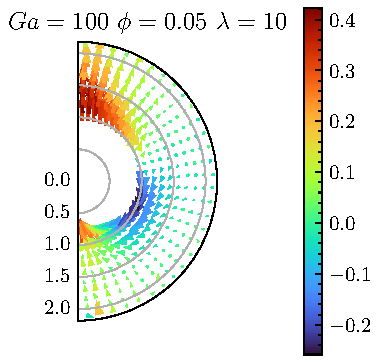
\includegraphics[height=0.35\textwidth]{image/HOMOGENEOUS_NEW/Dist/U_l_10_Ga_100_PHI_5.pdf}
    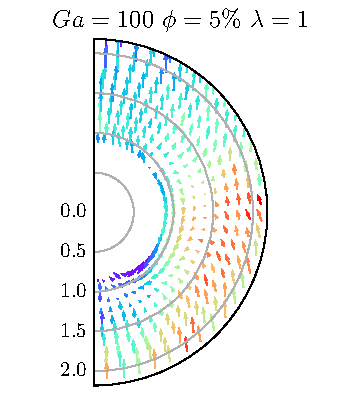
\includegraphics[height=0.35\textwidth]{image/HOMOGENEOUS_NEW/Dist/U_l_1_Ga_100_PHI_5.pdf}
    \caption{
         Quiver plots of the conditioned particle velocity field $\textbf{u}^\text{r}(\textbf{x},\textbf{r},t)$ colored by the averaged dimensionless vertical velocity difference : $(\textbf{u}^\text{r} - \textbf{u}_p )/ \textbf{u}_p$, for $\phi = 0.05$ and $Ga = 100$. 
         (left) High viscosity ratio $\lambda = 10$.
         (right) Low viscosity ratio, $\lambda = 1$.
         }
    \label{fig:unst_l}
\end{figure}
On \ref{fig:unst_l} (left) we first notice that $\textbf{u}^\text{r}(\textbf{x},\textbf{r},t)$ behave similarly as the low inertial case display on \ref{fig:unst_ga} (left).
However, for $\lambda = 10$, the isolated particles' velocity is roughly equal to $\textbf{u}_p$. 
If isolated particle rise at the average velocity it is because the isolated particles constitute the majority of the realization since the trace of \textbf{R} is rather high, see \ref{fig:A}.
Therefore, this fact is not particularly relevant as it is just a statistical bias. 
Nevertheless, we can still conclude that for $\lambda = 10$ particles goes faster with a nearest neighbor on top or bottom, while for  $\lambda = 1$ particles goes faster when the nearest neighbor is at large distance. 


\subsubsection*{Discussion}

From \ref{sec:time} we demonstrated that $\textbf{R}(\textbf{x},t)$ follows a transport equation were the tensor $\textbf{W}(\textbf{x},t)$ act as a source term. 
This tensor might be expressed as the symmetric part of $\int_0^\infty \textbf{r} \textbf{w}_p^\text{r} P(\textbf{x},\textbf{r},t) da$. 
Thus, the trends of the $\textbf{w}_p^\text{r}(\textbf{x},\textbf{r},t) $ in terms of the position determine the value of $\textbf{W}(\textbf{x},t)$ and partly determine the final value of $\textbf{R}(\textbf{x},t)$. 
In most of the graphs we observed that the vertical components of $\textbf{w}_p^\text{r}$ where negative when the vertical component of where positive \textbf{r} and vice versa. 
Consequently, $W_{yy}$ must be on average negative, which ultimately contribute to the value of $\textbf{R}(\textbf{x},t)$ and $\textbf{A}(\textbf{x},t)$ through \ref{eq:dt_R} and justify the sign of $A_{xx}$ in \ref{fig:A}. 

% On a different note, we now ask this question : 
% Is the relative velocity fields $\textbf{w}_p^r$ is the cause of the microstructure's shape as it is suggested by \ref{eq:dt_R}. 
% Or does $\textbf{w}_p^r$ is the consequence of microstructure shape, as it could be through looking at the previous graphs ?
% Indeed, on \ref{fig:Why_l_matter} (right), the clear asymmetry with respect to the horizontal plane can be explained as the consequence of cluster  in the flows. 
% Although it is tedious question, we believe that both are true, even if physical parameters also impact $\textbf{w}_p^r$, which makes the microstructure case dependent.  
% Nevertheless, this makes $\textbf{W}(\textbf{x},t)$ potentially a function of $\textbf{R}(\textbf{x},t)$.
% Depending on its relationship with $\textbf{R}(\textbf{x},t)$ this might modify the relaxation time.  
% Thus, a more efficient way to close \textbf{W} by an objective manner would be to study the dynamic of interactions. 
In this work we only provided a kinematics arguments to explain the microstructure shape. 
Of course to fully understand the physics one has to study the dynamic of interaction. 
It is in fact possible in our framework to include such dynamic variable by deriving an equation for \textbf{W} the same way we derived \ref{eq:dt_R} for \textbf{R}.
% In this case it is reasonable to believe that the closure terms for the dynamical equation might be computable theoretically in terms of the physical parameters $Ga$, $\phi$ and $\lambda$. 

% \subsection{Carrier phase velocity fields}

In the previous section we explained the microstructure formation with kinematic arguments.
Although we indeed provided an explanation the question that arise now id :
Why does the relative velocity behave as such.
The answer might be obtained based on dynamical arguments as it is done often, in such a way we could explain the relative kinematic.
Nevertheless, the dynamical aspect of the interaction is out of the scope of this study and will be treated in a future work. 

Instead, we propose to study the particles averaged wakes to explain the possible difference in interaction between the iso-viscous and viscous droplets cases. 
Again we make use of the nearest particle averaged statistic to compute the carrier fluid phase velocity conditionally on the presence of a particle at \textbf{x}, it reads,
\begin{equation*}
    \textbf{u}^\text{nst}_f P_{nst}(\textbf{x},\textbf{r},t)= 
    \int \sum_{i}^{N_b} \delta(\textbf{x}-\textbf{x}_i(\FF,t))
    h_{i} 
    \textbf{u}_f^0(\textbf{x}+\textbf{r},t,\FF)
    d\mathscr{P} 
\end{equation*}
where $h_{i} = 1$ if the particle $i$ center of mass is the nearest point to the eularian coordinate \textbf{x}+\textbf{r}. 
This velocity fields can be reconstructed as well with our DNS. 
On \ref{fig:stream} we display the reconstructed velocity field $\textbf{u}^\text{nst}_f$ for (left) the iso-viscous case $\lambda =1$ and (right) the viscous droplets' case $\lambda = 10$, for different value of the volume fraction. 
\begin{figure}[h!]
    \centering
    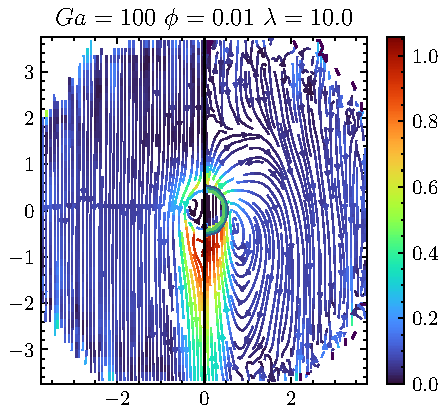
\includegraphics[height=0.4\textwidth]{image/HOMOGENEOUS_NEW/Stream/Stream_PHI_1_Ga_100_l_100}
    \includegraphics[height=0.4\textwidth]{image/HOMOGENEOUS_NEW/Stream/Stream_PHI_1_Ga_100_l_10}
    \includegraphics[height=0.4\textwidth]{image/HOMOGENEOUS_NEW/Stream/Stream_PHI_5_Ga_5_l_100}
    \includegraphics[height=0.4\textwidth]{image/HOMOGENEOUS_NEW/Stream/Stream_PHI_5_Ga_5_l_10}
    \includegraphics[height=0.4\textwidth]{image/HOMOGENEOUS_NEW/Stream/Stream_PHI_20_Ga_100_l_100}
    \includegraphics[height=0.4\textwidth]{image/HOMOGENEOUS_NEW/Stream/Stream_PHI_20_Ga_100_l_10}
    % \includegraphics{image/HOMOGENEOUS_NEW/Stream/Stream_PHI_5_Ga_100_l_1.pdf}
    \caption{Nearest averaged carrier phase velocity fields. }
    \label{fig:stream}
\end{figure}
This velocity field is evaluated at $\textbf{x}+\textbf{r}$ conditioned on the presence of the nearest particle at $\textbf{x}$. 


\tb{compare with \citet{shajahan2023inertial} for explaination }
% 






\subsection{Nearest particles arrangements}
\begin{itemize}
    \item Problematic : "How the particles are arranged relative to each other"
    \item Show : "How to compute the Radial and azimuthal probability density function : $P_{nst}(r)$  and $P_{nst}(\theta)$"
    \item  Conclusion on $P_{nst}(\theta)$ : "We observe that the particles pair becomes oriented with increasing $Ga$ and decreasing volume fraction.
    \item  Conclusion on $P_{nst}(r)$ : "We observe that the particles pair becomes randomly arranged for high $Ga$ but in average they are rather spaced from each other" 
\end{itemize}
\tb{Je me demande si cette section est vraiment utile .... car elle n'apport pas d'explication supplementaire a la drag force ni aux fluctuations, c'est peux être mieux de garder ca pour l'article qui traîte des interactions }


\subsubsection{Map at low $Ar$}

\paragraph{low $\phi$}
\begin{figure}
\centering
\includegraphics[width=4cm]{image/HOMOGENEOUS/fDrop/Pnst_mu_r_0_1_Ga_10_PHI_0_05}
\includegraphics[width=4cm]{image/HOMOGENEOUS/fDrop/Pnst_mu_r_1_0_Ga_10_PHI_0_05}
\end{figure}

\JL{a on la meme echelle de couleur entre les deux graphiques, les cas Ga=5 ne semblent pas converger ? a virer ...}

Pas de position preferentiel dans ce cas

\paragraph{high $\phi$}
\begin{figure}
\centering
\includegraphics[width=4cm]{image/HOMOGENEOUS/fDrop/Pnst_mu_r_0_1_Ga_10_PHI_0_15}
\includegraphics[width=4cm]{image/HOMOGENEOUS/fDrop/Pnst_mu_r_1_0_Ga_10_PHI_0_15}
\end{figure}

Idem pas de position preferentiel a discuter a la lumiere de la litterature (qui tends a dire le contraire ?). En regime de Stokes pas d'effet significatif du rapport de viscosité sur les pertubations. 







\subsubsection{Map at high $Ar$}

\paragraph{low $\phi$}
\begin{figure}
\centering
\includegraphics[width=4cm]{image/HOMOGENEOUS/fDrop/Pnst_mu_r_0_1_Ga_75_PHI_0_05}
\includegraphics[width=4cm]{image/HOMOGENEOUS/fDrop/Pnst_mu_r_1_0_Ga_75_PHI_0_05}
\end{figure}

enorme effet du rapport de viscosité (donc a priori du sillage).
\JL{il manque des cas a Ga=100 ?}


\paragraph{high $\phi$}
\begin{figure}
\centering
\includegraphics[width=4cm]{image/HOMOGENEOUS/fDrop/Pnst_mu_r_0_1_Ga_75_PHI_0_15}
\includegraphics[width=4cm]{image/HOMOGENEOUS/fDrop/Pnst_mu_r_1_0_Ga_75_PHI_0_15}
\end{figure}

\subsubsection{...}


\begin{figure}
    \centering
    \begin{tikzpicture}
        \node at (0,0){ \includegraphics[height=0.3\textwidth]{image/HOMOGENEOUS/fDrop/Pnst_theta_mu_r_1_0_Ga_10.pdf} };
        \node at (0.4\textwidth,0){ \includegraphics[height=0.3\textwidth]{image/HOMOGENEOUS/fDrop/Pnst_theta_mu_r_0_1_Ga_10.pdf} };
        \node at (0,-0.3\textwidth){ \includegraphics[height=0.3\textwidth]{image/HOMOGENEOUS/fDrop/Pnst_theta_mu_r_1_0_Ga_75.pdf} };
        \node at (0.4\textwidth,-0.3\textwidth){ \includegraphics[height=0.3\textwidth]{image/HOMOGENEOUS/fDrop/Pnst_theta_mu_r_0_1_Ga_100.pdf} };
        % \node at (0,-0.6\textwidth){ \includegraphics[height=0.3\textwidth]{image/HOMOGENEOUS/fDrop/Pnst_theta_mu_r_1_0_Ga_100.pdf} };
        % \node at (0.4\textwidth,-0.6\textwidth){ \includegraphics[height=0.3\textwidth]{image/HOMOGENEOUS/fDrop/Pnst_theta_mu_r_0_1_Ga_100.pdf} };
    \end{tikzpicture}
    \caption{Probability density function of the nearest particles : $P_{nst}(\theta)$ for different $Ga$ and $\lambda$. 
    Increasing $Ga$ from top to bottom, (left) $\lambda = 1$ (right) $\lambda = 10$. 
    The symbols correspond to different volume fraction ($\bullet$) $\phi = 1\%$, ($\blacktriangle$) $\phi = 5\%$, ($\blacksquare$) $\phi = 10\%$, ($\blacklozenge$) $\phi = 15\%$ and ($\blacktriangleright$) $\phi = 20\%$.
    (dashed lines) empirical formulas }
    \label{fig:P_nst_theta}
\end{figure}
By using polar coordinate such that $d \textbf{r} = r^2 \sin \phi dr d\phi d\theta$ we can further reduce the PDF to the only consideration of the angular dependency $\theta$ or the distance dependency $r$. 
These reduced p.d.f can be computed as follow, 
\begin{align*}
    P_{nst}(r) 
    &= \int_{-\pi/2}^{\pi/2}\int_{0}^{2\theta} P_{nst}(\textbf{x},\textbf{r},t) \sin \theta  d\phi d\theta\\
    P_{nst}(\theta)
    &= \int_{0}^{\infty}\int_{0}^{2\theta} P_{nst}(\textbf{x},\textbf{r},t) r^2  dr d\phi
\end{align*}
\tb{Check if those formulas are true}
Then $P_{nst}(\theta)$ is the probability that the nearest neighbor of a test particle is inclined at an angle $\theta$ relative to the flow direction. 
We observe that the particles pair becomes oriented with increasing $Ga$ and decreasing volume fraction

On \ref{fig:P_nst_theta} we observe that the particles pair becomes oriented with increasing $Ga$ and decreasing volume fraction.
Indeed, we observe a clear peak of $P_{nst}(\theta)$ at $\theta = \frac{\pi}{2}$. 
It seems that this tendency was also reported for spherical bubble in air-water system \citet{bunner2003effect}. 
Additionally, from \ref{fig:P_nst_theta} we can say that the viscosity ratio $\lambda$ seem to prevent the alignment/clustering of particles denoted by the slightly low peak for $\lambda =10$. 
\tb{Compart the Orientation with bubbly and solid flows \citet{roghair2011drag}}

\begin{figure}
    \centering
    \begin{tikzpicture}
        \node at (0,0){ \includegraphics[height=0.3\textwidth]{image/HOMOGENEOUS/fDrop/Pnst_r_mu_r_1_0_PHI_1.pdf} };
        \node at (0.4\textwidth,0){ \includegraphics[height=0.3\textwidth]{image/HOMOGENEOUS/fDrop/Pnst_r_mu_r_0_1_PHI_1.pdf} };
        \node at (0,-0.3\textwidth){ \includegraphics[height=0.3\textwidth]{image/HOMOGENEOUS/fDrop/Pnst_r_mu_r_1_0_PHI_10.pdf} };
        \node at (0.4\textwidth,-0.3\textwidth){ \includegraphics[height=0.3\textwidth]{image/HOMOGENEOUS/fDrop/Pnst_r_mu_r_0_1_PHI_10.pdf} };
        \node at (0,-0.6\textwidth){ \includegraphics[height=0.3\textwidth]{image/HOMOGENEOUS/fDrop/Pnst_r_mu_r_1_0_PHI_20.pdf} };
        \node at (0.4\textwidth,-0.6\textwidth){ \includegraphics[height=0.3\textwidth]{image/HOMOGENEOUS/fDrop/Pnst_r_mu_r_0_1_PHI_20.pdf} };
    \end{tikzpicture}
    \caption{Radial probability density function : $P_{nst}(r)$ for different $\phi$ and $\lambda$. 
    Increasing $\phi$ from top to bottom, (left) $\lambda = 1$ (right) $\lambda = 10$. 
    The symbols correspond to different Galileo number ($\bullet$) $Ga = 10$, ($\blacktriangle$) $Ga = 25$, ($\blacksquare$) $Ga = 50$, ($\blacklozenge$) $Ga = 75$ and ($\blacktriangleright$) $Ga = 100$.
    (dashed lines) Theoretical formula \ref{eq:P_nst_r}}
    \label{fig:P_nst_r}
\end{figure}
Note that for solid spherical particle in the dilute regime a theoretical formula for $P_{nst}(r)$ can be found assuming completely random distribution and no interactions nor overlap between particles \citep{zhang2021ensemble}, it reads, 
\begin{equation*}
    P_\text{nst}^\text{th}(r) = n_p e^{-4 \pi n_p (r^3 - d^3)/3}.
    \label{eq:P_nst_r}
\end{equation*}
It is evident that all the distribution presented \ref{fig:P_nst_r} have a peak at $r > 1$ where the theoretical formula  predict a peak at $r=1$. 
This is obviously due to the fact that we are in presence of particles interaction which tends to repulse the particles from each others and therefore to shift the distribution to the left. 
What is more interesting is that for $\lambda = 1$ at low volume fraction and high \textit{Galileo} we are able to recover approximately the random particle distribution $P_\text{nst}^\text{th}$ with our numerical results. 
Whereas for $\lambda = 10$ the particle are relatively maintained far from  each other as depicted \ref{fig:P_nst_r}(right). 
We can stipulate that for high viscosity ratio the particles have a tendency to generate more particle fluid mediated interaction as demonstrated by the flow lines \ref{fig:Stream}.


\subsection{Nearest-particle average fluid velocity}
Objectives : 
\begin{itemize}
    \item Problematic "How to analyse the flow around a particle in average"
    \item First : present the averaged the nearest particles' statistics method. And how to compute the nearest averaged velocity fields $\nstavg{\textbf{u}}$.
    \item Present the flowlines and show that for $\phi = 5 \rightarrow 20\%$ we observe that a vertical symmetry arise.
    \item Explain how this field it is related to the velocity fluctuation with \ref{eq:def_uu}
    \item Conclude that these velocity fields represent the PWFs since it represent the mean wakes \citep{du2022analysis}.  
    \item Additionally, some comment can be made regarding the shape of the particle thanks to the contour lines. 
    \item Approach these flow fields by analytical solution of potential flow to obtain an analytical solution for teh reyolds stress. 
\end{itemize}

Presently, we wish to investigate the  averaged flow structure around a fluid particle.
To obtain such a field we make use of the nearest particle statistics recently introduced by \citet{zhang2021stress}. 
We introduce $\nstavg{\textbf{u}}(\textbf{x},\textbf{r})$ as the velocity fields at \textbf{x} knowing there is a particles center of mass located at \textbf{r}.
Additionally, this particle is the nearest particle among all to the point \textbf{x}.  
Formally, this conditional average can be written as, 
\begin{equation}
    \nstavg{\textbf{u}}(\textbf{x},\textbf{r})=\frac{1}{P_{nst}(\textbf{x},\textbf{r})} 
    \int \textbf{u}(\textbf{x},\CC,t) 
    \sum_{\alpha}\delta(\textbf{x}+\textbf{r}-\textbf{x}^\alpha(\CC,t)) h_{\alpha}(\CC,\textbf{x},t) d\mathscr{P} 
    \label{eq:q_nst_avg}
\end{equation}
where $P_{nst}(\textbf{x},\textbf{r})$ is defined as,  
\begin{equation}
    P_{nst}(\textbf{x},\textbf{r})= 
    \int
    \sum_{\alpha}\delta(\textbf{x}+\textbf{r}-\textbf{x}^\alpha(\CC,t)) 
    h_\alpha(\CC,\textbf{x},t) d\mathscr{P}. 
    \label{eq:P_nsti}
\end{equation}
which is the probability of finding a particle center of mass at a distance \textbf{r} from the point \textbf{x} knowing that this particle is the nearest neighbor to the points \textbf{x}. 
The function $h_\alpha$ is defined such that, $h_\alpha = 1/N^p$ if $\alpha$ is the nearest particle to \textbf{x} and $0$ if not, where $N^p$ is the total number of nearest neighbor.
Indeed, the point \textbf{x} at mid-distance from two particles posses two nearest neighbors by definition, thus $N(\textbf{x},\CC,t) = 2$ in this case. 

\tb{Include the numerical computaiton of $\nstavg{\textbf{u}}$.  }

\ref{fig:Stream} shows the streamline of the field $\nstavg{\textbf{u}}(\textbf{x},\textbf{r})$ for three volume fractions. 
We clearly observe the induced wake of the particles centered at the origin. 

\begin{figure}[h!]
    \centering
    \begin{tikzpicture}
        \node (img) at (0,0)  {\includegraphics[height=0.3\textwidth]{image/HOMOGENEOUS/Stream/Stream_PHI_20_Ga_10_l_1.pdf}};
        \node (img) at (0.3\textwidth,0)  {\includegraphics[height=0.3\textwidth]{image/HOMOGENEOUS/Stream/Stream_PHI_20_Ga_50_l_1.pdf}};
        \node (img) at (0.6\textwidth,0)  {\includegraphics[height=0.3\textwidth]{image/HOMOGENEOUS/Stream/Stream_PHI_20_Ga_100_l_1.pdf}};
        \node (img) at (0,-0.3\textwidth)  {\includegraphics[height=0.3\textwidth]{image/HOMOGENEOUS/Stream/Stream_PHI_20_Ga_10_l_10.pdf}};
        \node (img) at (0.3\textwidth,-0.3\textwidth)  {\includegraphics[height=0.3\textwidth]{image/HOMOGENEOUS/Stream/Stream_PHI_20_Ga_50_l_10.pdf}};
        \node (img) at (0.6\textwidth,-0.3\textwidth)  {\includegraphics[height=0.3\textwidth]{image/HOMOGENEOUS/Stream/Stream_PHI_20_Ga_100_l_10.pdf}};
        \node (img) at (0,-0.6\textwidth)  {\includegraphics[height=0.3\textwidth]{image/HOMOGENEOUS/Stream/Stream_PHI_5_Ga_10_l_1.pdf}};
        \node (img) at (0.3\textwidth,-0.6\textwidth)  {\includegraphics[height=0.3\textwidth]{image/HOMOGENEOUS/Stream/Stream_PHI_5_Ga_50_l_1.pdf}};
        \node (img) at (0.6\textwidth,-0.6\textwidth)  {\includegraphics[height=0.3\textwidth]{image/HOMOGENEOUS/Stream/Stream_PHI_5_Ga_100_l_1.pdf}};
        \node (img) at (0,-0.9\textwidth)  {\includegraphics[height=0.3\textwidth]{image/HOMOGENEOUS/Stream/Stream_PHI_5_Ga_10_l_10.pdf}};
        \node (img) at (0.3\textwidth,-0.9\textwidth)  {\includegraphics[height=0.3\textwidth]{image/HOMOGENEOUS/Stream/Stream_PHI_5_Ga_50_l_10.pdf}};
        \node (img) at (0.6\textwidth,-0.9\textwidth)  {\includegraphics[height=0.3\textwidth]{image/HOMOGENEOUS/Stream/Stream_PHI_5_Ga_100_l_10.pdf}};
    \end{tikzpicture}
    \caption{Nearest particle averaged velocity $\nstavg{\textbf{u}}(\textbf{r})$ for  $\phi = 5\%$ and $20\%$.
    Green lines : contour plots of the nearest averaged indicator function $\nstavg{\chi_d}(\textbf{r})$ (it represent the mean shape of the particles)}
    \label{fig:Stream}
\end{figure}
% \begin{figure}[h!]
%     \centering
%     \begin{tikzpicture}
%         \node (img) at (0,0)  {\includegraphics[height=0.4\textwidth]{image/HOMOGENEOUS/Stream/P_PHI_5_Ga_10_l_1.pdf}};
%         \node (img) at (0.3\textwidth,0)  {\includegraphics[height=0.4\textwidth]{image/HOMOGENEOUS/Stream/P_PHI_5_Ga_50_l_1.pdf}};
%         \node (img) at (0.6\textwidth,0)  {\includegraphics[height=0.4\textwidth]{image/HOMOGENEOUS/Stream/P_PHI_5_Ga_100_l_1.pdf}};
%         \node (img) at (0,0.4\textwidth)  {\includegraphics[height=0.4\textwidth]{image/HOMOGENEOUS/Stream/P_PHI_20_Ga_10_l_10.pdf}};
%         \node (img) at (0.3\textwidth,0.4\textwidth)  {\includegraphics[height=0.4\textwidth]{image/HOMOGENEOUS/Stream/P_PHI_5_Ga_50_l_10.pdf}};
%         \node (img) at (0.6\textwidth,0.4\textwidth)  {\includegraphics[height=0.4\textwidth]{image/HOMOGENEOUS/Stream/P_PHI_5_Ga_100_l_10.pdf}};
%     \end{tikzpicture}
%     \caption{Nearest particle averaged pressure $\nstavg{p}(\textbf{r})$ normalized by the Laplace pressure $4 \gamma /d$ for  $\phi = 5\%$ and $20\%$}
%     \label{fig:Stream}
% \end{figure}
\begin{figure}[h!]
    \centering
    \begin{tikzpicture}
        \node (img) at (0,0)  {\includegraphics[height=0.3\textwidth]{image/HOMOGENEOUS/Stream/P_PHI_20_Ga_10_l_1.pdf}};
        \node (img) at (0.3\textwidth,0)  {\includegraphics[height=0.3\textwidth]{image/HOMOGENEOUS/Stream/P_PHI_20_Ga_50_l_1.pdf}};
        \node (img) at (0.6\textwidth,0)  {\includegraphics[height=0.3\textwidth]{image/HOMOGENEOUS/Stream/P_PHI_20_Ga_100_l_1.pdf}};
        \node (img) at (0,-0.3\textwidth)  {\includegraphics[height=0.3\textwidth]{image/HOMOGENEOUS/Stream/P_PHI_20_Ga_10_l_10.pdf}};
        \node (img) at (0.3\textwidth,-0.3\textwidth)  {\includegraphics[height=0.3\textwidth]{image/HOMOGENEOUS/Stream/P_PHI_20_Ga_50_l_10.pdf}};
        \node (img) at (0.6\textwidth,-0.3\textwidth)  {\includegraphics[height=0.3\textwidth]{image/HOMOGENEOUS/Stream/P_PHI_20_Ga_100_l_10.pdf}};
        \node (img) at (0,-0.6\textwidth)  {\includegraphics[height=0.3\textwidth]{image/HOMOGENEOUS/Stream/P_PHI_5_Ga_10_l_1.pdf}};
        \node (img) at (0.3\textwidth,-0.6\textwidth)  {\includegraphics[height=0.3\textwidth]{image/HOMOGENEOUS/Stream/P_PHI_5_Ga_50_l_1.pdf}};
        \node (img) at (0.6\textwidth,-0.6\textwidth)  {\includegraphics[height=0.3\textwidth]{image/HOMOGENEOUS/Stream/P_PHI_5_Ga_100_l_1.pdf}};
        % \node (img) at (0,-0.9\textwidth)  {\includegraphics[height=0.3\textwidth]{image/HOMOGENEOUS/Stream/P_PHI_5_Ga_10_l_10.pdf}};
        \node (img) at (0.3\textwidth,-0.9\textwidth)  {\includegraphics[height=0.3\textwidth]{image/HOMOGENEOUS/Stream/P_PHI_5_Ga_50_l_10.pdf}};
        \node (img) at (0.6\textwidth,-0.9\textwidth)  {\includegraphics[height=0.3\textwidth]{image/HOMOGENEOUS/Stream/P_PHI_5_Ga_100_l_10.pdf}};
    \end{tikzpicture}
    \caption{Nearest particle averaged pressure $\nstavg{p}(\textbf{r})$ normalized by the Laplace pressure $4 \gamma /d$ for  $\phi = 5\%$ and $20\%$}  
    \label{fig:Stream}
\end{figure}
It is evident from these plots that the induced wake is the averaged wake resulting from the averaged translation of the particles. 
And this averaged wake has a tendency to be asymmetrical for low volume fraction and symmetrical for higher ones. 
Additionally, form basic mathematical consideration on the average operators we can demonstrate that :
\begin{multline*}
    \avg{\chi_k \textbf{u}'_k\textbf{u}'_k}(\textbf{x},t)
    + \phi_k \textbf{u}_k\textbf{u}_k
    = \\
    \underbrace{\int (\nstavg{\chi_k \textbf{u}^0_k}  \nstavg{\chi_k \textbf{u}^0_k} / (\nstavg{\chi_k})  P_{nst}(\textbf{x},t,\textbf{r}) d\textbf{r} }_\text{PWFs}
    +\underbrace{\int \nstavg{\chi_k \textbf{v}_k^0\textbf{v}_k^0}  P_{nst}(\textbf{x},t,\textbf{r}) d\textbf{r}}_\text{WIA}
    \label{eq:def_uu}
\end{multline*}
where, $\textbf{v}_k^0  = \textbf{u}_k^0 - \nstavg{\chi_k \textbf{u}^0_k} / \nstavg{\chi_k}$ is the fluctuation of the local velocity relative to the nearest averaged value. 
Consequently, we can decompose the ensemble averaged fluid velocity fluctuations with a first term representing the variance of $\nstavg{\textbf{u}}$ around the mean $\textbf{u}_k$, and a second term representing the variance of $\textbf{u}^0_k$ around the mean  $\nstavg{\textbf{u}}$. 

There are two phenomena causing velocity fluctuations in the liquid:
the agitation resulting from wakes and their collective interactions [wake-induced agitation (WIA)], and the non-turbulent fluctuations resulting from averaged wakes and potential flows around bubbles [potential flow and averaged wake fluctuations (PWFs)].
As a matter of fact in the phase space of $\nstavg{\textbf{u}}(\textbf{r})$ the bubble is fixed at the origin thus we recover the velocity fields representing what is called the PWFs. 
In their study \citet{du2022analysis} carry out transient simulation with fixed particles to recover the PWFs components here we show that a single simulation permit us to recover WIA and PWFs by the mean of the nearest particles' statistics. 

\tb{make the link with drag force/drag coef  \citet{dandy1989buoyancy}}
\tb{make the link with velocity fluctuation \citet{almeras2021statistics}}





\subsection{Nearest averaged particle center of mass velocity}
\subsubsection{Nearest averaged particle center of mass velocity in the dispersed phase reference frame}
\begin{equation}
    \nstavg{\textbf{u}^i}=\frac{1}{P_{nst}(\textbf{x},\textbf{r},t)} 
    \int \sum_{i}\delta(\textbf{x}-\textbf{x}^i(\CC,t))
    \sum_{j\neq i}\delta(\textbf{x}+\textbf{r}-\textbf{x}^j(\CC,t)) 
    % \delta(t+a-t_c^{ij}(\CC,t)) 
    h_{ij}(\CC,t) 
    \textbf{u}^i(\CC,t)
    d\mathscr{P} 
    - \textbf{u}_p
\end{equation}
\subsubsection{Nearest averaged particle center of mass relative velocity}
\begin{equation}
    \nstavg{\textbf{w}}=\frac{1}{P_{nst}(\textbf{x},\textbf{r},t)} 
    \int \sum_{i}\delta(\textbf{x}-\textbf{x}^i(\CC,t))
    \sum_{j\neq i}\delta(\textbf{x}+\textbf{r}-\textbf{x}^j(\CC,t)) 
    % \delta(t+a-t_c^{ij}(\CC,t)) 
    h_{ij}(\CC,t) 
    (\textbf{u}^i(\CC,t) - \textbf{u}^j(\CC,t))
    d\mathscr{P} 
\end{equation}


\begin{figure}[h!]
    \centering
    \begin{tikzpicture}
        \node (img) at (0,0)  {\includegraphics[height=0.3\textwidth]{image/HOMOGENEOUS/fDrop/U_l_1_Ga_10_PHI_20.pdf}};
        \node (img) at (0.3\textwidth,0)  {\includegraphics[height=0.3\textwidth]{image/HOMOGENEOUS/fDrop/U_l_1_Ga_50_PHI_20.pdf}};
        \node (img) at (0.6\textwidth,0)  {\includegraphics[height=0.3\textwidth]{image/HOMOGENEOUS/fDrop/U_l_1_Ga_100_PHI_20.pdf}};
        \node (img) at (0,-0.3\textwidth)  {\includegraphics[height=0.3\textwidth]{image/HOMOGENEOUS/fDrop/U_l_10_Ga_10_PHI_20.pdf}};
        \node (img) at (0.3\textwidth,-0.3\textwidth)  {\includegraphics[height=0.3\textwidth]{image/HOMOGENEOUS/fDrop/U_l_10_Ga_50_PHI_20.pdf}};
        \node (img) at (0.6\textwidth,-0.3\textwidth)  {\includegraphics[height=0.3\textwidth]{image/HOMOGENEOUS/fDrop/U_l_10_Ga_100_PHI_20.pdf}};
        \node (img) at (0,-0.6\textwidth)  {\includegraphics[height=0.3\textwidth]{image/HOMOGENEOUS/fDrop/U_l_1_Ga_10_PHI_5.pdf}};
        \node (img) at (0.3\textwidth,-0.6\textwidth)  {\includegraphics[height=0.3\textwidth]{image/HOMOGENEOUS/fDrop/U_l_1_Ga_50_PHI_5.pdf}};
        \node (img) at (0.6\textwidth,-0.6\textwidth)  {\includegraphics[height=0.3\textwidth]{image/HOMOGENEOUS/fDrop/U_l_1_Ga_75_PHI_5.pdf}};
        \node (img) at (0,-0.9\textwidth)  {\includegraphics[height=0.3\textwidth]{image/HOMOGENEOUS/fDrop/U_l_10_Ga_10_PHI_5.pdf}};
        \node (img) at (0.3\textwidth,-0.9\textwidth)  {\includegraphics[height=0.3\textwidth]{image/HOMOGENEOUS/fDrop/U_l_10_Ga_50_PHI_5.pdf}};
        \node (img) at (0.6\textwidth,-0.9\textwidth)  {\includegraphics[height=0.3\textwidth]{image/HOMOGENEOUS/fDrop/U_l_10_Ga_75_PHI_5.pdf}};
    \end{tikzpicture}
    \caption{Nearest particle averaged pressure velocity $\nstavg{\textbf{u}^i}(\textbf{r}) - \textbf{u}_p$ }  
    \ref{fig:u_nst}
\end{figure}
% \begin{figure}[h!]
%     \centering
%     \begin{tikzpicture}
%         \node (img) at (0,0)  {\includegraphics[height=0.3\textwidth]{image/HOMOGENEOUS/fDrop/U_rel_l_1_Ga_10_PHI_20.pdf}};
%         \node (img) at (0.3\textwidth,0)  {\includegraphics[height=0.3\textwidth]{image/HOMOGENEOUS/fDrop/U_rel_l_1_Ga_50_PHI_20.pdf}};
%         \node (img) at (0.6\textwidth,0)  {\includegraphics[height=0.3\textwidth]{image/HOMOGENEOUS/fDrop/U_rel_l_1_Ga_100_PHI_20.pdf}};
%         \node (img) at (0,-0.3\textwidth)  {\includegraphics[height=0.3\textwidth]{image/HOMOGENEOUS/fDrop/U_rel_l_10_Ga_10_PHI_20.pdf}};
%         \node (img) at (0.3\textwidth,-0.3\textwidth)  {\includegraphics[height=0.3\textwidth]{image/HOMOGENEOUS/fDrop/U_rel_l_10_Ga_50_PHI_20.pdf}};
%         \node (img) at (0.6\textwidth,-0.3\textwidth)  {\includegraphics[height=0.3\textwidth]{image/HOMOGENEOUS/fDrop/U_rel_l_10_Ga_100_PHI_20.pdf}};
%         \node (img) at (0,-0.6\textwidth)  {\includegraphics[height=0.3\textwidth]{image/HOMOGENEOUS/fDrop/U_rel_l_1_Ga_10_PHI_5.pdf}};
%         \node (img) at (0.3\textwidth,-0.6\textwidth)  {\includegraphics[height=0.3\textwidth]{image/HOMOGENEOUS/fDrop/U_rel_l_1_Ga_50_PHI_5.pdf}};
%         \node (img) at (0.6\textwidth,-0.6\textwidth)  {\includegraphics[height=0.3\textwidth]{image/HOMOGENEOUS/fDrop/U_rel_l_1_Ga_75_PHI_5.pdf}};
%         \node (img) at (0,-0.9\textwidth)  {\includegraphics[height=0.3\textwidth]{image/HOMOGENEOUS/fDrop/U_rel_l_10_Ga_10_PHI_5.pdf}};
%         \node (img) at (0.3\textwidth,-0.9\textwidth)  {\includegraphics[height=0.3\textwidth]{image/HOMOGENEOUS/fDrop/U_rel_l_10_Ga_50_PHI_5.pdf}};
%         \node (img) at (0.6\textwidth,-0.9\textwidth)  {\includegraphics[height=0.3\textwidth]{image/HOMOGENEOUS/fDrop/U_rel_l_10_Ga_75_PHI_5.pdf}};
%     \end{tikzpicture}
%     \caption{Nearest particle averaged pressure velocity $\nstavg{\textbf{w}}(\textbf{r})$ }  
%     \ref{fig:w_nst}
% \end{figure}
o

\section{Conclusion}
\section{Conclusion}

% \citet{einstein1905neue,taylor1932viscosity} demonstrated how the first moment of the hydrodynamic forces (Stresslet) applied on a particle immersed in pure linear flow induced an additional viscosity to the mixture. 
% Later~\citet{zhang1994ensemble,lhuillier1996contribution,jackson1997locally,zhang1997momentum} demonstrated that the second moment of forces were also contributing to the stresses inducing a non-newtonian behaviors, even in the Stokes and dilute limit.  

In this work we computed the moments of force on the surface of a test droplet in the situation of uniform relative motions between the droplet and the continuous phase. 
We considered low but finite Reynolds number $Re$. 
The averaged first moment of force is given by~\ref{eq:forces_reformulated2_avg}, scales as $O(\rho_f \phi u_r^2)$, hence contributing to the averaged Stress of the suspension on the same ground as  \citet{einstein1905neue} or \citep{taylor1932viscosity} correction to the viscosity of the mixture. 
In a lesser extend the inertial part of the second moment also contribute to the Rheology. 
This first point constitutes the main result of the paper. 

Others important conclusion reached through this work includes: a general reciprocal formula to derive the forces and moments on droplets, and the explicit appearing of the velocity variance term in the drag force term. 







\appendix
%\section{Statistical convergence and mesh independence studies}
\section{Numerical validations}
\label{ap:validation}
The \texttt{Basilisk} code has been validated numerous time in previous numerical studies. 
Especially, we can cite the recent studies of \citet{innocenti2020direct} and \citet{hidman2023assessing} which both performed DNS of rising suspension of bubbles. 
Nevertheless, in this work we investigate specific statistical distribution,
and we make use of a multi-VoF method to avoid droplets coalescence, therefore a meticulous validation of the DNS is in order. 
We start by presenting a brief comparison with the reference DNS \citet{esmaeeli1999direct}. 
Afterward we present a study focusing on the interfaces' kinematic, we compare our DNS with the experimental results of \citet{mohamed2003drop} in the objective to show that the Multi-VoF method indeed capture the physics of two colliding interfaces without solving the flows in the film. 
Once the mesh and the physics are validated, a study on the convergence of the statistics is presented. 

\subsection*{Ordered array of buoyant bubbles}

From our knowledge, no simulations nor experimental results have been carried out for rising buoyant viscous drop. 
Therefore, instead we reproduced the ordered array simulation of \citet{esmaeeli1999direct} with \texttt{Basilisk} to validate the mesh definition of our DNS.  
It consists in a 3-D buoyant ordered rising array of bubbles. 
In our notation the flow parameters of the simulation reads, 
\begin{align*}
    \lambda = 10,
    && \zeta = 10,
    && Bo = 1.8,
    && Ga = 28.37,
    && \phi = 0.125.
\end{align*}
\begin{figure}[h!]
    \centering
    \includegraphics[height = 0.3\textwidth]{image/VALIDATION2.0/Loisy/Re.pdf}
    \caption{Time evolution of the Reynolds number based on the instentaneous volume averaged drift velocity, $Re(t) = \rho_fU d /\mu_f$, with $U(t) = |\textbf{u}_p - \textbf{u}_f|$ with $\phi = 0.1256$, $\zeta =\mu_r =10$ and $Ga = 29.9$.
    $\textbf{u}_p$ and $\textbf{u}_f$ are the particle and fluid phase volume averaged velocity at time $t$.}
    \label{fig:ordered_array}
\end{figure}
\ref{fig:ordered_array} display our numerical simulation against the original result of \citet{esmaeeli1999direct}.
We observe very good agreements between both studies for all mesh definition.
Additionally, we displayed the results of \citet{innocenti2020direct} for $d/\Delta = 20$ to point out a divergence with our results at the same mesh definition.  
Both our simulations and the one of \citet{innocenti2020direct} have been carried out with the  \texttt{Basilisk} code. 
The cause of this difference is in fact due to a different method of interpolation used for the viscosity coefficient $\mu$. 
We used an arithmetic mean, whereas \citet{innocenti2020direct} used a 
harmonic mean.
As a matter of fact in this regime the arithmetic mean, which will be used in this work, permit us to reach a faster convergence. 
Overall these results indicate that the criterion $d/\Delta = 30$ seems sufficient, which is consistent with the aforementioned studies.


\subsection*{Drop impact on a liquid-liquid interface}

In section, we investigate in more detail the physics behind the Multi-VoF method. 
We need to verify if we accurately capture the physics of the droplets interfaces despite the fact that we do not model accurately  the film between two droplets. 
Following \citet{balcazar2015multiple} we reproduced the experiment of drop impact on a liquid–liquid interface carried by \citet{mohamed2003drop} but with the \texttt{Basilisk} code. 
This experiment consist in letting a drop fall into a pool of the same fluid as the drop, all along the experiment the interfaces of the droplets and the pool are tracked. 
In our notation the dimensionless parameters of latter study reads, 
\begin{align*}
    Ga = 71.02 
    && Bo = 6.40
    && \lambda = 0.33
    && \zeta = 1.189
\end{align*}
Following \citet{mohamed2003drop} we defined the dimensionless time $t / t_i = t U_i(t) /d$ where $U_i(t)$ is droplet velocity at $t<0$ and where $t=0$ is the time of impact. 
Regarding the geometry of the problem we sketched in \ref{fig:schemeLong} a scheme of the initial position of the droplet in the computational domain.
Additionally, we displayed on \ref{fig:schemeLong} a snapshot of the numerical domain were we see the drop colliding the pool's interface.
Both, the drop and the pool does not merge since we use the Multi-VoF method, note that in the experiment the drop does not merge with the pool either.
This enables us to represent with DNS a physical situation where the interfaces do not coalesce, but where we use a grid definition of $d/\Delta = 30$ which is of course not sufficient to model the flow inside the film. 
\begin{figure}[h!]
    \centering
    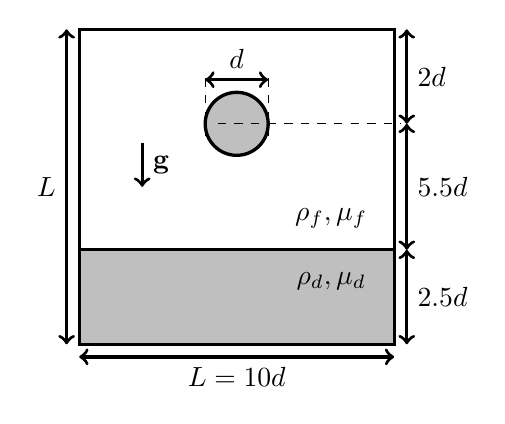
\begin{tikzpicture}[very thick,scale = 0.8]
        \draw (0,0) rectangle (5,5);
        \draw[fill=gray!50] (0,0) rectangle (5,1.5);
        \draw[fill=gray!50] (2.5,3.5) circle (0.5);
        \draw[<->](0,-0.2) --++ (5,0)node[midway,below]{$L  = 10 d$};
        \draw[<->](-0.2,0) --++ (0,5)node[midway,left]{$L$};
        \draw[<->](5.2,0) --++ (0,1.5)node[midway,right]{$2.5 d$};
        \draw[<->](5.2,1.5) --++ (0,2)node[midway,right]{$5.5 d$};
        \draw[<->](5.2,3.5) --++ (0,1.5)node[midway,right]{$ 2d$};
        \draw[dashed,thin](2.2,3.5) --++ (2.9,0);
        \draw[dashed,thin](2.2,3.5) --++ (2.9,0);
        \draw[->](1,3.2) --++ (0,-0.7)node[midway,right]{$\textbf{g}$};
        \draw[<->](2,4.2) --++ (1,0)node[midway,above]{$d$};
        \draw[thin,dashed](2,3.3) --++ (0,1);
        \draw[thin,dashed](3,3.3) --++ (0,1);
        \node (a) at (4,2){$\rho_f, \mu_f$};
        \node (a) at (4,1){$\rho_d, \mu_d$};
    \end{tikzpicture}
    \includegraphics[height = 0.3\textwidth]{image/VALIDATION2.0/Longmire/IMG/image-079.png}
    \caption{(left) Scheme of the computational set up at the initial time. 
    (right) Snapshot of the computational domain after the collision time, with the interfaces represented in gray.
    The background color represent the velocity field magnitude, which is undisturbed, indicating a large enough domain. }
    \label{fig:schemeLong}
\end{figure}
\begin{figure}[h!]
    \centering
    \includegraphics[height = 0.3\textwidth]{image/VALIDATION2.0/Longmire/Re.pdf}
    \includegraphics[height = 0.3\textwidth]{image/VALIDATION2.0/Longmire/Dist.pdf}
    \caption{(left) Time evolution of the Reynolds number based on the droplet velocity, $Re(t) = \rho_fU d /\mu_f$ in term of the dimensionless time, (+) numerical results of  \citet{balcazar2015multiple} (right)  position of the interfaces, ($\bullet$) top droplets surface, ($+$) bot droplet surface, (x) pool surface. (Symbols) experimental result of \citet{mohamed2003drop} (solid line) present numerical simulations with $d/\Delta = 30$. }
    \label{fig:resultslong}
\end{figure}
\ref{fig:resultslong} represent the comparison between our results against the experiment of \citet{mohamed2003drop} (right) and the numerical simulation of \citet{balcazar2015multiple} (left). 
The time dependent Reynolds number as well as the interfaces positions are shown to match exactly both, the numerical and experiential results of \citet{balcazar2015multiple} and \citet{mohamed2003drop}, respectively. 
From the very good agreement obtained with the numerical and experimental results we conclude that the kinematic is preserved during the contact time for a mesh definition of $d/\Delta = 30$. 

\subsection*{Mesh independence and statistical convergence for random array of drops}

Even through aforementioned studies carried validation of the \texttt{Basilisk} code for rising droplets or bubbles, almost all of them considered isolated droplets or bubbles as the only validation case. 
As far as the author's knowledge, to this date no published study presented a mesh independence study for random array of droplets nor bubbles of this scale. 
Nevertheless, as particles interaction and higher \textit{Galileo} numbers may be more challenging to model, it is primordial to investigate the mesh independence of the exact same DNS that are carried in this work. 
In this objective we performed DNS of random array of $N_b=125$ droplets, with the following parameters,
\begin{align*}
    \lambda = 10,
    && \zeta = 1.11,
    && Bo = 1,
    && Ga = 100,
    && \phi = 0.1,
    && N_b =125,
\end{align*}
and the mesh definition is, $d/\Delta = 7.37, 14.74, 29.9 58.97$. 
We expect that the most challenging DNS simulated in this work is for the case, $\lambda = 10$ and $Ga = 100$, since it is in this range of parameters that we induce the most vorticity, which ultimately require good mesh definition. 
Additionally, in opposition to the ordered array case, this case includes droplets interaction, which ultimately induce more numerical complexities to tackles. 
Based on this remark we can assume that if this case is mesh independent, then all cases from \ref{tab:simulations} must be since this is the most challenging scenario.   

Let's first verify the independence of the drift velocity on the mesh definition. 
\begin{figure}[h!]
    \centering
    \includegraphics[height = 0.3\textwidth]{image/HOMOGENEOUS_NEW/VAL/Re.pdf}
    \caption{
        Time evolution of the Reynolds number based on the instantaneous volume averaged drift velocity, $Re(t) = \rho_fU d /\mu_f$, with $U(t) = |\textbf{u}_p - \textbf{u}_f|$ with $\phi = 0.1256$, $\zeta =\mu_r =10$ and $Ga = 29.9$ for different mesh definition.
        $\textbf{u}_p$ and $\textbf{u}_f$ are the particle and fluid phase volume averaged velocity at time $t$.
        In the legend we display the value of the mesh definition and of the ensemble averaged Reynolds number. 
    }
    \label{fig:Re}
\end{figure}
In \ref{fig:Re} we display the instantaneous volume averaged drift velocity in terms of time, for four mesh definition. 
The results are not as independent of the mesh definition as the order array validation presented above. 
Indeed, we observe a difference of the rising Reynolds number of about $5\%$ between the $d/\Delta = 29.49$ and $d/\Delta = 58.97$ cases which is notable.
We recall that this $5\%$ error will eventually be lower for all other cases. 
The good agreement between the case  $d/\Delta = 14.74$ and $d/\Delta = 29.49$ is partially fortuitous.

Now let's study the mesh influence on the statistics. 
It is clear from \ref{fig:apstat} (left) that both mesh definition produce nearly the same radial distribution, no notable difference is identified. 
In \ref{fig:ap_age} (middle) we can observe the age distribution for both mesh definition. 
It is clear that refining the mesh induce a difference in the age distribution. 
As, a matter of fact it has a small impact on the mean age, $\tau_p = 6.96$ for the lower definition, and $\tau_p = 6.14$ for the finest grid.
This makes a $10\%$ error, but as mentioned above this is probably the highest error that we could encounter among all cases. 
\begin{figure}
    \centering
    \includegraphics[height = 0.24\textwidth]{image/HOMOGENEOUS_NEW/VAL/Pr.pdf}
    \includegraphics[height = 0.24\textwidth]{image/HOMOGENEOUS_NEW/VAL/Pa.pdf}
    \includegraphics[height = 0.24\textwidth]{image/HOMOGENEOUS_NEW/VAL/w.pdf}
    \caption{
        Statistical averaged functions for two mesh definition. 
        (left) Radial normalized probability density function  $P_r(\textbf{x},|\textbf{r}|,t)/P_\text{th}$, in terms of the dimensionless radial position. 
        (middle) Probability density function of the age distribution $P_a(\textbf{x},t,a)$. 
        (right) Nearest averaged dimensionless approach velocity for both mesh definition, in terms of the dimensionless age. 
    }
    \label{fig:apstat}
\end{figure}
Even through an error is identified on the mean age of interaction we still notice that both nearest averaged dimensionless approach velocity on \ref{fig:apstat} (right) match perfectly. 
\begin{figure}[h!]
    \centering
    \includegraphics[height = 0.3\textwidth]{image/HOMOGENEOUS_NEW/VAL/U_rel_ndc_25.pdf}
    \includegraphics[height = 0.3\textwidth]{image/HOMOGENEOUS_NEW/VAL/U_rel_ndc_35.pdf}
    \caption{Quiver plots of the relative averaged velocity field $\textbf{w}^\text{r}(\textbf{x},\textbf{r},t)$ colored by the averaged dimensionless age $a^r(\textbf{x},\textbf{r},t)$, for $\phi = 0.05$ and $Ga = 100$. 
    (left) Low mesh definition.
    (right) High mesh definition. 
    }
    \label{fig:velap}
\end{figure}
Regarding, the 2D fields  $\textbf{w}^\text{r}(\textbf{x},\textbf{r},t)$ we can see that no notable difference can be identified, if it is not the slight difference in the value of the age scale. 


Overall, the one dimensional and two-dimensional conditioned statistics are almost independent of the mesh definition. 
By obtaining the same statistics with two independent DNS makes us confident on the fact that our numerical samples is large enough.
Indeed, if the samples were not sufficient we would have obtained two different distribution functions, thus we can be sure that the statistics have well converged. 
The slight difference in rising velocity and age distribution found for these Reynolds number must be acknowledged.
As mentioned at the beginning, this case is in fact very challenging as the volume fraction of droplets is consequent which induce numerous inertial interactions. 
Nevertheless, we can be sure that our final results is accurate at most with a $5\%$ error for this case, and probably less for the others cases. 
Overall, we have great confidence in the statistical and physical representativity of our DNS results. 
% 
% \subsection{Statistical and mesh independence study}
\tb{Should i put the number of realization is abs $\omega$}

In the aim of providing accurate closure terms it is of primary importance to verify the well convergence of the mean quantities, either by varing the mesh definition domain size and duration of simulation.
To tackle this problem we carried out four simulation with 125 rising droplets with different mesh definition. 
The flow parameters for this validation read as,  
\begin{align*}
    \mu_r = 0.1,
    && \rho_r = 1.11,
    && Bo = 1,
    && Ga = 75,
    && \phi = 0.1,
    && N_b =125. 
\end{align*}
Note that in these simulations we used a number of $125$ droplets.  
In \ref{ap:A} we give more details on this choice and show that for our concerns it is a sufficient number of droplets. 

\ref{fig:Re_and_Tc}(left) display the cumulative mean of the vertical Reynolds number based on the drift velocity, namely,
\begin{equation}
    \widetilde{Re}(t)
    = \frac{\rho_f d}{\mu_f t}\int_{t_0}^{t_0+t} \left(\Xavg{\textbf{u}^0_d} -  \Xavg{\textbf{u}_c^0}\right)dt'
\end{equation}
\tb{ time average and volume average}
where $t_0$ is the starting sampling time. 
We remark a significant dependence of $\tilde{Re}$ with the mesh definition in contrast to the latter study (see \ref{fig:ordered_array}). 
It is hard to distinguish the cause of this difference, if it is not just because of the presence of interaction between droplets. 
Anyhow, we reach mesh independent results for $d/\Delta \geq 30$ in agreements with the recent studies of \citet{loisy2017buoyancy} \citet{zhang2021direct} for low inertial bubbly flows.
Also, $\widetilde{Re}$ reaches a constant values from $t^* = 50$. 
This is true for all mesh definition.  
Consequently, we reached an accurate time convergence for the rising velocity. 
\begin{figure}[h!]
    \centering
    % \includegraphics[height = 0.3\textwidth]{image/VALIDATION2.0/fCA/Re.pdf}
    \includegraphics[height = 0.3\textwidth]{image/VALIDATION2.0/fCA/Recum.pdf}
    \includegraphics[height = 0.3\textwidth]{image/VALIDATION2.0/fCA/Tcum.pdf}
    % \includegraphics[height = 0.35\textwidth]{image/VALIDATION2.0/fPA/Tcum.pdf}
    \caption{(left) Cumulative mean of the volume averaged Reynolds number along the simulation time based on the drift velocity $U = \textbf{u}_p - \textbf{u}_c$, with $\phi = 0.1$, $\rho_r = 1.11$, $ \mu_r =0.1$ and $Ga = 29.9$ and $N_b = 125$.
    (right) Cumulative mean of the fluid Reynolds stress tesor. }
    \label{fig:Re_and_Tc}
\end{figure}

The well convergence of the rising velocity doesn't guarantee a statistical nor a mesh convergence for finer quantities such as the pseudo-turbulent kinetic energy. 
Therefore, we provide on \ref{fig:UpUp} (left) the running average of the fluid phase pseudo-turbulent energy. 
Similarly, \ref{fig:UpUp} (right) represent the particle center of mass pseudo-turbulent kinetic energy. 
\begin{figure}[h!]
    \centering
    \includegraphics[height = 0.3\textwidth]{image/VALIDATION2.0/fCA/Tcum.pdf}
    \includegraphics[height = 0.3\textwidth]{image/VALIDATION2.0/fPA/Tcum.pdf}
    \caption{(left) Cumulative mean of the volume averaged granular temperature along the simulation time based on the drift velocity $U = \textbf{u}_p - \textbf{u}_c$, with $\phi = 0.1$, $\rho_r = 1.11$, $ \mu_r =0.1$ and $Ga = 29.9$ and $N_b = 125$.
    (right) Cumulative mean of the dimensionless particle-fluid-particle stress horizontal component tensor. }
    \label{fig:UpUp}
\end{figure}
Both figure exhibit well converged data. 
Interestingly, $\widetilde{K}_c$ and $\widetilde{K}_\alpha$ reach a constant value at $t^* = 200$ which is four time greater than for $\widetilde{Re}$.


\tb{this convergence can be compared to Loisy studies}
\tb{Cite and compare to Berner and \citet{bunner2002dynamics} which found that Nb > 12 is sufficient \citet{roghair2011drag}}
Now, let's investigate the required number of droplets per domain, $N_b$, and the minimum definition of cells per diameter of droplets $\delta$.  
\tb{Include bibliography and expectation here \ldots}
For this investigation we kept the physical parameters presented in the same section and made a double parametric analysis over $N$ and $\delta$. 
We carried out simulations for $N = 2, 3, 4, 5, 6, 7$, and for a number of cells $10 <\delta < 40$. 
In Basilisk the mesh definition is defined by a power of two, consequently depending on the size of the domain (which is fixed to keep a $\phi$ constant) the $\delta$ parameter is fixed at a power of 2 close. 
\begin{figure}[h!]
    \centering
    \includegraphics[height= 0.3\textwidth]{image/VALIDATION/N_and_delta/DUd.pdf}
    \includegraphics[height= 0.3\textwidth]{image/VALIDATION/N_and_delta/PHI.pdf}
    \caption{(left) Averaged Reynolds number based on the drift velocity.
            (right) Dispersed phase volume fraction at the end of each simulation.
            The text on the side of the points is $\delta$.
            N correspond to $N = N_b^3$. }
    \label{fig:VALIDATION_Nd_1}
\end{figure}
\ref{fig:VALIDATION_Nd_1}(left), illustrate clearly that the drift velocity is independent of the parameters $N_b$ and $\delta$, for $N >4$. 
On the other hand, \ref{fig:VALIDATION_Nd_1}(right), show that the volume fraction of the dispersed phase is lower for the low defined grid (red dots), due to a loss of volume during the simulation.
This doesn't mean that the solver isn't volume conservative. 
In fact, it is fund to be due to the \href{http://basilisk.fr/sandbox/fintzin/Rising-Suspension/no-coalescence.h}{no-coalescence.h} which generate fragment into the numerical domain, fragment which are deleted in the long run. 
\begin{figure}[h!]
    \centering
    \includegraphics[height= 0.3\textwidth]{image/VALIDATION/N_and_delta/PA_UpUp.pdf}
    \includegraphics[height= 0.3\textwidth]{image/VALIDATION/N_and_delta/Mh.pdf}
    \caption{(left) Fluids phase averaged fluctuation tensor.
            (right) Particular average of the first moment tensor, where $F_g$ is the buoyancy force applied on one droplet. 
            The numerical values displayed alongside the dots are the number of cells per diameter.}
    \label{fig:VALIDATION_Nd_2}
\end{figure}
Now, let's look at the behavior of more \textit{complicated} closure terms. 
\ref{fig:VALIDATION_Nd_2}(left) demonstrate that the vertical component of the pseudo turbulent tensor is parameter independent rather early, independently of the grid definition. 
This fact is rather surprising but note that the standard deviation is quite high for small domain. 
On \ref{fig:VALIDATION_Nd_2}(right), we can examine the vertical component of the first moment closure term. 
It is found to be constant for all $N$, but rather inaccurate for coarse grids. 
Which makes sens since the first moment results from a local calculation of the stress over a droplet volume, unlike the other quantities which results from the averaged center of mass velocity of a droplet. 

As we have shown, the quantities presented converge for a number of droplets equivalent to $N = 4$ and $\delta = 25$. 
Thus, we validate our simulation in space, i.e. we made sure that our domain were wide enough to minimize the influence of the periodicity on our results, and in mesh definition. 
Nevertheless, at it is the number of realization that matter when carrying a particular average, it is interesting to look at the duration of the simulation.


The last validation that we must expose is the convergence with the relative properties. 
Indeed, the film definition might change interaction properties such that the particle normal approach $\textbf{w}_n(a)$. 
\begin{figure}[h!]
    \centering
    \includegraphics[height=0.3\textwidth]{image/VALIDATION2.0/Hnst/ur_a_ndc_35_Ga_75.pdf}
    \caption{Normal approach Nearest particle velocity for different $Ga$. 
    We can see that for $\delta = 29,60$ we obtain the same results.}
\end{figure}




\section{Additional information}
\label{ap:age} 

\begin{figure}[h!]
  \centering
  \includegraphics[height = 0.3\textwidth]{image/HOMOGENEOUS_NEW/CA/Re_l_1.pdf}
  \includegraphics[height = 0.3\textwidth]{image/HOMOGENEOUS_NEW/CA/Re_l_10.pdf}
  \caption{
      Averaged Reynolds number based on the averaged drift velocity, $Re = \rho_fU d /\mu_f$, with $U = |\textbf{u}_p - \textbf{u}_f|$.
      $\textbf{u}_p$ and $\textbf{u}_f$ are the particle and fluid phase volume and time averaged velocity.
  }
  \label{fig:Reall}
\end{figure}

\begin{table}  
\begin{tabular}{c|c|c|c|l}
  calls  &  total  &   self  & \% total  & function \\ \hline
  10636901 &  4861.39 &  4861.39  &   31.8\% (28.4\% - 36.7\%) &   mpi\_boundary\_level():grid/multigrid-mpi.h:83\\
     53604 &  3097.64 &  1988.97  &   13.0\% (10.8\% - 14.7\%) &   project():poisson.h:501\\
     26802 &  2022.99 &  1236.57  &    8.1\% ( 7.3\% -  8.8\%) &   viscosity():viscosity.h:173\\
    107208 &  1984.59 &  1223.33  &    8.0\% ( 6.9\% -  8.9\%) &   heights():heights.h:281\\
     26802 &  2499.81 &  1099.66  &    7.2\% ( 6.1\% -  7.9\%) &   vof\_0():vof.h:365\\
   3155070 &  983.66  & 983.66    &  6.4\% ( 3.9\% -  9.1\%)   & mpi\_all\_reduce0():common.h:683\\
     26802 &  2372.23 &  896.09   &   5.9\% ( 5.1\% -  6.5\%)  &  advection\_term():navier-stokes/centered.h:323\\
     26802 &  1583.59 &  645.89   &   4.2\% ( 4.1\% -  4.3\%)  &  no\_coalescence():./no-coalescence.h:419\\
      2681 &  584.39  & 372.15    &  2.4\% ( 2.4\% -  2.5\%)   & track\_bub():RS.c:124\\
    321624 &  546.74  & 340.36    &  2.2\% ( 1.8\% -  2.6\%)   & reconstruction():fractions.h:476\\
    107208 &  2777.30 &  303.23   &   2.0\% ( 1.6\% -  2.4\%)  &  curvature():curvature.h:621\\
     69275 &  992.44  & 254.14    &  1.7\% ( 1.4\% -  1.8\%)   & tag():tag.h:268\\
     26802 &  328.67  & 202.85    &  1.3\% ( 1.1\% -  1.5\%)   & acceleration\_0():iforce.h:133\\
     26802 &  2257.27 &  178.19   &   1.2\% ( 0.8\% -  1.3\%)  &  projection():navier-stokes/centered.h:430\\
     26802 &  2142.30 &  119.30   &   0.8\% ( 0.5\% -  0.9\%)  &  viscous\_term():navier-stokes/centered.h:362\\
     26802 &  145.95  & 116.09    &  0.8\% ( 0.5\% -  0.9\%)   & acceleration\_2():RS.c:166\\
     26803 &  111.60  & 111.57    &  0.7\% ( 0.5\% -  0.8\%)   & properties\_0():two-phase-generic.h:101\\
     26802 &  172.09  & 100.18    &  0.7\% ( 0.5\% -  0.8\%)   & acceleration():navier-stokes/centered.h:386\\
     69275 &   68.91  &  68.88    &  0.5\% ( 0.4\% -  0.5\%)   & z\_indexing():grid/multigrid-mpi.h:145\\
       118 &   59.59  &  59.59    &  0.4\% ( 0.2\% -  0.8\%)   & compose\_image():view.h:409\\
     26802 &   64.69  &  34.48    &  0.2\% ( 0.2\% -  0.3\%)   & tracer\_advection\_1():./no-coalescence.h:446\\
        59 &  129.57  &  28.81    &  0.2\% ( 0.1\% -  0.2\%)   & movies():RS.c:244\\
     26803 &   92.48  &  27.24    &  0.2\% ( 0.1\% -  0.2\%)   & stability\_1():tension.h:64\\
     26803 &   24.42  &  21.33    &  0.1\% ( 0.1\% -  0.1\%)   & stability():navier-stokes/centered.h:226\\
  43894361 &  3001.24 &    5.50   &   0.0\% ( 0.0\% -  0.0\%)  &  boundary\_internal():grid/cartesian-common.h:450\\
  42061052 &   25.50  &   3.61    &  0.0\% ( 0.0\% -  0.0\%)   & interpolate():grid/cartesian-common.h:815\\
       472 &    2.31  &   2.31    &  0.0\% ( 0.0\% -  0.0\%)   & draw\_vof():draw.h:1052\\
     58554 &   25.92  &   0.87    &  0.0\% ( 0.0\% -  0.0\%)   & reduce\_bubbles():./no-coalescence.h:158\\
         1 &  15287.89&     0.73  &    0.0\% ( 0.0\% -  0.0\%) &   run():run.h:37\\
         1 &    0.28  &   0.28    &  0.0\% ( 0.0\% -  0.0\%)   & init\_0():RS.c:149\\
     26802 &  2777.57 &    0.27   &   0.0\% ( 0.0\% -  0.0\%)  &  acceleration\_1():tension.h:94\\
       236 &   38.81  &   0.21    &  0.0\% ( 0.0\% -  0.0\%)   & squares():draw.h:1375\\
    %    118 &   59.64  &   0.05    &  0.0\% ( 0.0\% -  0.1\%)   & save():view.h:529\\
    %  63404 &    0.06  &   0.03    &  0.0\% ( 0.0\% -  0.0\%)   & interpolate():grid/cartesian-common.h:816\\
    %      1 &    0.02  &   0.02    &  0.0\% ( 0.0\% -  0.0\%)   & defaults\_3():iforce.h:38\\
    %      1 &    0.01  &   0.01    &  0.0\% ( 0.0\% -  0.0\%)   & defaults\_2():two-phase-generic.h:26\\
    %  26802 &  1583.60 &    0.01   &   0.0\% ( 0.0\% -  0.0\%)  &  vof\_1():./no-coalescence.h:430\\
    %  26802 &    0.01  &   0.01    &  0.0\% ( 0.0\% -  0.0\%)   & set\_dtmax():navier-stokes/centered.h:222\\
    %  26803 &    0.00  &   0.00    &  0.0\% ( 0.0\% -  0.0\%)   & stability\_0():vof.h:143\\
    %      1 &    0.25  &   0.00    &  0.0\% ( 0.0\% -  0.0\%)   & init():navier-stokes/centered.h:213\\
    %      1 &    0.00  &   0.00    &  0.0\% ( 0.0\% -  0.0\%)   & defaults\_0():navier-stokes/centered.h:181\\
    %      1 &    0.00  &   0.00    &  0.0\% ( 0.0\% -  0.0\%)   & restore():output.h:1169\\
    %      1 &    0.00  &   0.00    &  0.0\% ( 0.0\% -  0.0\%)   & cleanup():run.h:52\\
    %      1 &    0.00  &   0.00    &  0.0\% ( 0.0\% -  0.0\%)   & defaults():run.h:44\\
    %      1 &    0.00  &   0.00    &  0.0\% ( 0.0\% -  0.0\%)   & defaults\_4():./no-coalescence.h:483\\
    %      1 &    0.00  &   0.00    &  0.0\% ( 0.0\% -  0.0\%)   & defaults\_1():vof.h:134\\
    %      1 &    0.00  &   0.00    &  0.0\% ( 0.0\% -  0.0\%)   & cleanup\_0():./no-coalescence.h:458\\
    %      1 &    0.00  &   0.00    &  0.0\% ( 0.0\% -  0.0\%)   & default\_display():navier-stokes/centered.h:188\\
    %      1 &    0.00  &   0.00    &  0.0\% ( 0.0\% -  0.0\%)   & stop():RS.c:272\\
\end{tabular}
\caption{Output of the basilisk compiler tool that measures algorithm performance all along the simulation.}
\label{tab:performance}
\end{table}


\begin{figure}[h!]
    \centering
    \includegraphics[height = 0.3\textwidth]{image/HOMOGENEOUS_NEW/PA/R.pdf}
    \caption{ First moment of the nearest particle pair distribution in the direction of gravity. 
    ($\pmb\bigcirc$) $\phi = 0.01$; ($\pmb\triangle$) $ \phi = 0.05$; ($\pmb\square$) $\phi = 0.1$ ($\pmb\lozenge$) $\phi = 0.2$.
    The hollow symbols correspond to $\lambda = 1$, the filled symbols to $\lambda = 10$.
    For $r<d$ we arbitrarily set $P_\text{r}^\text{th} = 1$ so that the distribution can be visualized.
    Black symbols represent the results of \citet{zhang2023evolution} for hard sphere suspension with $\phi = 0.016,0.056,0.134,0.262$  %$\phi = 0.0168,0.0565,0.1341,0.2622$ 
    corresponding to $\pmb\times,\pmb +, \pmb\star , \pmb\triangledown$, respectively.
    }
    \label{fig:ap:RY}
\end{figure}

\begin{figure}
  \centering
  \includegraphics[height = 0.3\textwidth]{image/HOMOGENEOUS_NEW/PA/rm.pdf}
  \caption{Dimensionless radial distance to the nearest neighbor for a random distribution.}
  \label{fig:ap:agee}
\end{figure}

\bibliography{Bib/bib_bulles.bib}




\end{document}

